% ============================================================
% PD-Inputs Deep Reference — shared preamble
% Single source of truth for packages, colors, tcolorbox envs.
% Chapters MUST use only the envs defined here. No ad-hoc colors.
% ============================================================

\documentclass[11pt,openany]{book}

\usepackage[a4paper,margin=1in]{geometry}
\usepackage[T1]{fontenc}
\usepackage{lmodern}
\usepackage{microtype}
\usepackage{amsmath,amssymb,amsthm}
\usepackage{siunitx}
\usepackage{xcolor}
\usepackage{graphicx}
\usepackage{enumitem}
\usepackage{booktabs}
\usepackage{array}
\usepackage{listings}
\usepackage{csquotes}
\usepackage{hyperref}
\usepackage[most]{tcolorbox}
\usepackage{tikz}
\usepackage{pgfplots}
\pgfplotsset{compat=1.18}
\usetikzlibrary{
  arrows.meta, positioning, calc, fit, shapes.geometric, shapes.misc,
  shadows, backgrounds, decorations.pathreplacing, decorations.markings,
  patterns, matrix, chains, automata
}

\hypersetup{
  colorlinks=true, linkcolor=blue!50!black, urlcolor=blue!50!black,
  citecolor=blue!50!black, pdfborder={0 0 0}
}

% ---------- Semantic color mapping (do not reuse for other purposes) ----------
\definecolor{cTLDR}{HTML}{6A3D9A}      % purple  — chapter payload
\definecolor{cKEY}{HTML}{1F77B4}       % blue    — single most important sentence
\definecolor{cPAUSE}{HTML}{17BECF}     % cyan    — mid-chapter recap
\definecolor{cHOOK}{HTML}{F2C200}      % yellow  — memory hook / mnemonic
\definecolor{cGUT}{HTML}{6F7378}       % gray    — gut check (retrieval)
\definecolor{cCHECK}{HTML}{2CA02C}     % green   — checkpoint
\definecolor{cPIT}{HTML}{D62728}       % red     — watch out
\definecolor{cPD}{HTML}{E67E22}        % orange  — why X cares
\definecolor{cSIDE}{HTML}{2F2F2F}      % black   — optional depth

% ---------- tcolorbox envs ----------
\newtcolorbox{tldr}[1][TL;DR]{
  enhanced, breakable, colback=cTLDR!6, colframe=cTLDR,
  coltitle=white, fonttitle=\bfseries, title={#1},
  left=4pt, right=4pt, top=4pt, bottom=4pt,
  attach boxed title to top left={xshift=8pt, yshift=-8pt},
  boxed title style={colback=cTLDR, sharp corners},
  arc=2pt
}

\newtcolorbox{keyidea}[1][Key Idea]{
  enhanced, breakable, colback=cKEY!8, colframe=cKEY,
  coltitle=white, fonttitle=\bfseries, title={#1},
  attach boxed title to top left={xshift=8pt, yshift=-8pt},
  boxed title style={colback=cKEY, sharp corners}, arc=2pt
}

\newtcolorbox{pausebox}[1][Pause]{
  enhanced, breakable, colback=cPAUSE!8, colframe=cPAUSE,
  coltitle=white, fonttitle=\bfseries, title={#1},
  attach boxed title to top left={xshift=8pt, yshift=-8pt},
  boxed title style={colback=cPAUSE, sharp corners}, arc=2pt
}

\newtcolorbox{hook}[1][Memory hook]{
  enhanced, breakable, colback=cHOOK!12, colframe=cHOOK!80!black,
  coltitle=black, fonttitle=\bfseries, title={#1},
  attach boxed title to top left={xshift=8pt, yshift=-8pt},
  boxed title style={colback=cHOOK, sharp corners}, arc=2pt
}

\newtcolorbox{gut}[1][Gut check]{
  enhanced, breakable, colback=cGUT!8, colframe=cGUT,
  coltitle=white, fonttitle=\bfseries, title={#1},
  attach boxed title to top left={xshift=8pt, yshift=-8pt},
  boxed title style={colback=cGUT, sharp corners}, arc=2pt
}

\newtcolorbox{checkpoint}[1][Checkpoint]{
  enhanced, breakable, colback=cCHECK!8, colframe=cCHECK,
  coltitle=white, fonttitle=\bfseries, title={#1},
  attach boxed title to top left={xshift=8pt, yshift=-8pt},
  boxed title style={colback=cCHECK, sharp corners}, arc=2pt
}

\newtcolorbox{pitfall}[1][Watch Out]{
  enhanced, breakable, colback=cPIT!8, colframe=cPIT,
  coltitle=white, fonttitle=\bfseries, title={#1},
  attach boxed title to top left={xshift=8pt, yshift=-8pt},
  boxed title style={colback=cPIT, sharp corners}, arc=2pt
}

\newtcolorbox{pdnote}[1][Why PD Cares]{
  enhanced, breakable, colback=cPD!10, colframe=cPD,
  coltitle=white, fonttitle=\bfseries, title={#1},
  attach boxed title to top left={xshift=8pt, yshift=-8pt},
  boxed title style={colback=cPD, sharp corners}, arc=2pt
}

\newtcolorbox{sidebar}[1][Sidebar: optional depth, skip if tired]{
  enhanced, breakable, colback=cSIDE!4, colframe=cSIDE,
  coltitle=white, fonttitle=\bfseries, title={#1},
  attach boxed title to top left={xshift=8pt, yshift=-8pt},
  boxed title style={colback=cSIDE, sharp corners}, arc=2pt
}

% ---------- Convenience macros ----------
\newcommand{\gutans}[1]{\par\smallskip{\small\color{cGUT}\textit{#1}}}
\newcommand{\mnemonic}[1]{\textbf{Say it in 2 seconds:} \textbf{\textit{#1}}}
\newcommand{\move}[1]{\paragraph{Move #1.}}

% Listings style for SDC / Liberty / LEF / DEF / Verilog snippets
\lstdefinestyle{eda}{
  basicstyle=\ttfamily\small, breaklines=true, frame=single,
  framerule=0.4pt, rulecolor=\color{black!40},
  backgroundcolor=\color{black!3}, columns=fullflexible,
  keywordstyle=\color{cKEY}\bfseries,
  commentstyle=\color{cCHECK!60!black}\itshape,
  stringstyle=\color{cPIT!70!black},
  numbers=left, numberstyle=\tiny\color{black!50}, numbersep=6pt
}
\lstset{style=eda}

\title{\textbf{Physical Design Inputs}\\[0.5em]\large A Deep Reference}
\author{Compiled for Kaushik Vada}
\date{\today}


\begin{document}

\frontmatter
\maketitle

\chapter*{How to Read This Book}
\addcontentsline{toc}{chapter}{How to Read This Book}

This book is a reference, not a transcript. Each chapter takes one Physical Design input artifact and goes deeper than the source lecture, with worked numbers, diagrams, and tight chunking. Read it the same way you would read a textbook chapter you actually intend to remember.

\bigskip
\noindent\textbf{The callout boxes are a language. Learn them once.}

\begin{itemize}[leftmargin=*]
  \item \textbf{TL;DR (purple)} opens every chapter with the payload in 3 to 4 bullets. From Chapter 8 onward, the first bullet is a callback to the prior chapter so the spaced repetition stays warm.
  \item \textbf{Memory hook (yellow)} gives you a vivid, sensory analogy. The brain remembers weird better than tidy.
  \item \textbf{Gut check (gray)} asks a question. \textbf{Cover the gray answer with your hand and try to recall first.} The recall attempt is the point, not the answer.
  \item \textbf{Pause (cyan)} is a mid-chapter recap. If you can repeat the Pause back to yourself, keep reading. If not, scroll back.
  \item \textbf{Key Idea (blue)} is the single most important sentence of the chapter. Underline it mentally.
  \item \textbf{Watch Out (red)} is a common mistake. These are the things interviewers ask about.
  \item \textbf{Why PD Cares (orange)} translates the chapter into three lenses: Arm PD internship, generic foundry-flow PD engineer, and VLSI interview prep.
  \item \textbf{Sidebar (black)} is optional depth. Skip if tired. Come back when curious.
  \item \textbf{Checkpoint (green)} closes the chapter with a 2-second mnemonic. If you can say the mnemonic aloud, the chapter is yours.
\end{itemize}

\bigskip
\noindent\textbf{Rule for when something is not clicking.} Scroll back to the most recent Pause or Memory hook and re-read from there. The book is built so that retreating one box is always enough to recover momentum.

\bigskip
\noindent\textbf{Rule for the Interview-ready 90-second answer at the back.} Cover it. Recite your own answer out loud. Then uncover and compare. This is the testing effect; it is the cheapest retention boost available.

\tableofcontents

\mainmatter

% =====================================================================
% Body chapters (one per PD input artifact)
% =====================================================================
\chapter{Physical Design Inputs: The Big Picture}

\begin{tldr}
\begin{itemize}[leftmargin=1.2em]
  \item A Physical Design (PD) job is fed by \textbf{six artifact families}: a gate-level \textbf{netlist}, an \textbf{SDC} constraints file, a \textbf{LEF} (Library Exchange Format), one or more \textbf{.lib} timing views, a \textbf{Technology file} (often with an ITF parasitic file plus mapping), and a \textbf{DEF} (Design Exchange Format) for floorplan and ports.
  \item Each input encodes a different question. Drop one and a different stage of the flow goes blind: synthesis hand-off, floorplanning, timing, parasitic extraction, or DRC all rely on a specific artifact.
  \item Modern advanced-node designs do not consume one .lib. They consume \textbf{dozens of .lib views across PVT corners and modes} (MMMC). The same is true for LEFs and parasitic tech views at multiple metal stacks.
  \item This chapter is the map. Chapters 8 onward zoom into each artifact one at a time.
\end{itemize}
\end{tldr}

\section*{An interview question you cannot dodge}

\begin{hook}[Hook]
A fresher walks into an Arm PD interview. First question: ``Tell me every file you would expect on your disk before you can run a single \texttt{floorplan} command.'' Silence in the room. The candidate names two files. The interviewer waits. Six were expected. Why six, and not one giant database?
\end{hook}

The instinct is to imagine one master file. In reality, six separate artifacts get handed to PD because each one is \textbf{authored by a different team and consumed by a different engine}. The netlist is a synthesis output. The .lib is a foundry signoff deliverable. The LEF is a library characterization output. The SDC is written by the architect or front-end lead. The tech file is foundry IP. The DEF is something PD itself iterates on. \textbf{Six origins, six update cadences, six file formats.}

\begin{keyidea}
Physical design is not a single tool ingesting a single file. It is a \textbf{pipeline of engines} (synthesis hand-off, floorplan, placement, CTS, route, signoff) where each engine demands a specific input that no other input can substitute for. Lose one, lose that engine.
\end{keyidea}

\section{The six inputs at a glance}

\begin{figure}[h]
\centering
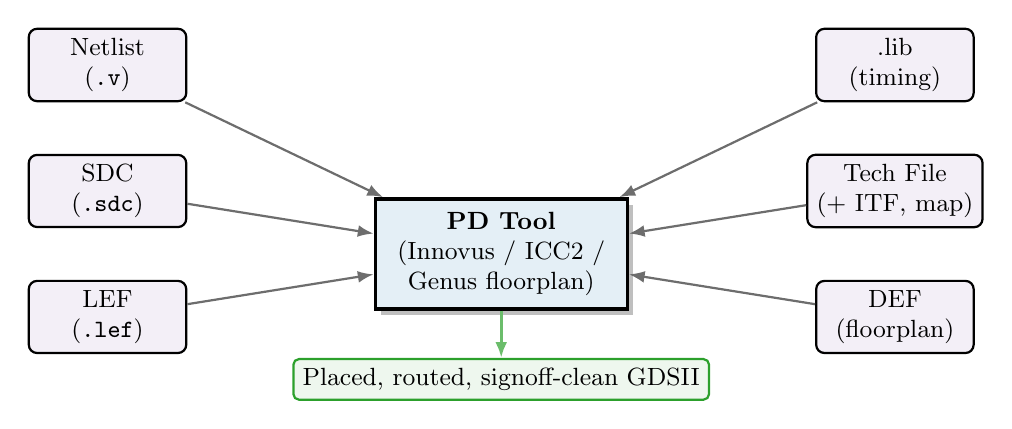
\begin{tikzpicture}[
  font=\small,
  artifact/.style={draw, rounded corners=3pt, minimum width=2.0cm, minimum height=0.8cm, align=center, fill=cTLDR!8, thick},
  tool/.style={draw, rectangle, minimum width=3.2cm, minimum height=1.4cm, align=center, fill=cKEY!12, very thick, drop shadow},
  arr/.style={-{Latex[length=2mm]}, thick, draw=cSIDE!70}
]
\node[tool] (pd) at (5,0) {\textbf{PD Tool}\\(Innovus / ICC2 /\\Genus floorplan)};

\node[artifact] (nl)  at (0,2.4)  {Netlist\\(\texttt{.v})};
\node[artifact] (sdc) at (0,0.8)  {SDC\\(\texttt{.sdc})};
\node[artifact] (lef) at (0,-0.8) {LEF\\(\texttt{.lef})};
\node[artifact] (lib) at (10,2.4) {.lib\\(timing)};
\node[artifact] (tf)  at (10,0.8) {Tech File\\(+ ITF, map)};
\node[artifact] (def) at (10,-0.8){DEF\\(floorplan)};

\draw[arr] (nl)  -- (pd);
\draw[arr] (sdc) -- (pd);
\draw[arr] (lef) -- (pd);
\draw[arr] (lib) -- (pd);
\draw[arr] (tf)  -- (pd);
\draw[arr] (def) -- (pd);

\node[draw=cCHECK, thick, rounded corners=2pt, fill=cCHECK!8, below=0.6cm of pd, align=center, minimum width=5cm]
  (out) {Placed, routed, signoff-clean GDSII};
\draw[arr, very thick, draw=cCHECK!70] (pd) -- (out);
\end{tikzpicture}
\caption{The six PD input artifacts feeding a single PD tool invocation. Authored upstream, consumed downstream, all required before signoff.}
\label{fig:pd-inputs-flow}
\end{figure}

\begin{hook}
Think of the PD tool as a \textbf{surgeon in an operating theater who refuses to cut until six specific trays of instruments are laid out by name}. Hand the surgeon five trays and they walk out. The sixth missing tray is not a warning, it is a hard stop.
\end{hook}

\subsection{What each artifact actually encodes}

\begin{figure}[h]
\centering
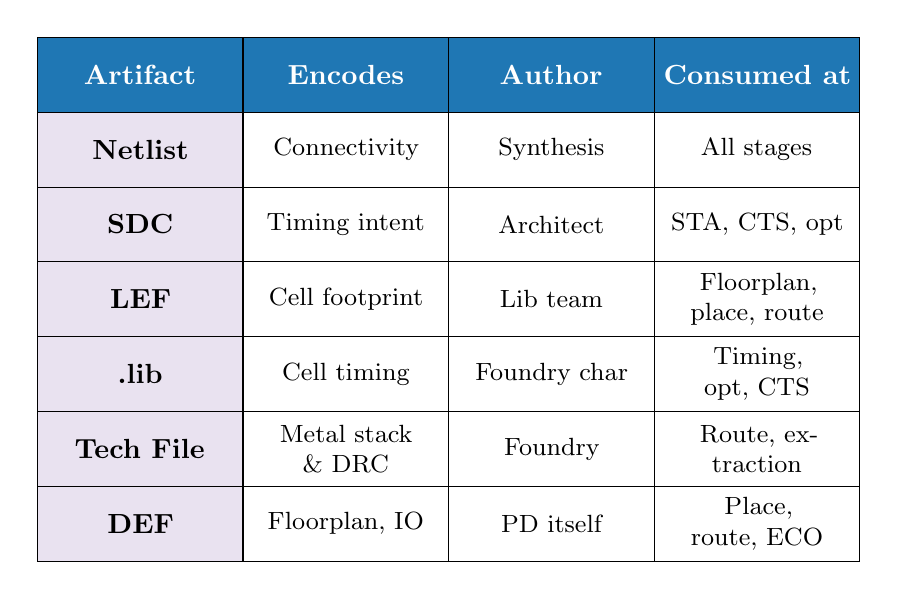
\begin{tikzpicture}[font=\small]
\matrix (m) [
  matrix of nodes,
  nodes={draw, anchor=center, text width=2.4cm, align=center, minimum height=0.95cm, inner sep=3pt},
  row 1/.style={nodes={fill=cKEY, text=white, font=\bfseries}},
  column 1/.style={nodes={fill=cTLDR!15, font=\bfseries}},
  row sep=-\pgflinewidth, column sep=-\pgflinewidth,
] {
  Artifact & Encodes        & Author       & Consumed at \\
  Netlist  & Connectivity   & Synthesis    & All stages \\
  SDC      & Timing intent  & Architect    & STA, CTS, opt \\
  LEF      & Cell footprint & Lib team     & Floorplan, place, route \\
  .lib     & Cell timing    & Foundry char & Timing, opt, CTS \\
  Tech File& Metal stack \& DRC & Foundry  & Route, extraction \\
  DEF      & Floorplan, IO  & PD itself    & Place, route, ECO \\
};
\end{tikzpicture}
\caption{Each input answers a question no other input answers. The author column is why no single file could replace the set.}
\label{fig:pd-inputs-table}
\end{figure}

\begin{gut}
If you delete the LEF but keep the .lib, what is the very first PD command that breaks?
\gutans{Anything that needs to place a cell on the floorplan. The .lib knows the cell's \emph{timing}, but it does not know the cell's \emph{shape}. Placement needs width, height, pin locations, all of which live in the LEF. Timing analysis on an unplaced design might still run, but you cannot draw a single rectangle.}
\end{gut}

\section{Walking the six, one at a time}

\move{1} \textbf{Netlist.} A gate-level Verilog file enumerating every instance and every wire. This is the only file that says ``instance \texttt{u\_alu/add\_42} is a \texttt{NAND2\_X2} whose A pin connects to net \texttt{n1764}.'' Without it, the PD tool has no design to place.

\move{2} \textbf{SDC.} The Synopsys Design Constraints file. It carries clock definitions (period, uncertainty, skew, latency), I/O delays, false paths, multicycle paths, max-transition, max-cap, and other DRV limits. The architect says ``this block must close at 1.2~GHz with 80~ps uncertainty.'' That sentence becomes an SDC line.

\move{3} \textbf{LEF.} A physical abstract of every standard cell and macro. Cell name, shape, size, orientation, pin name, pin layer, pin geometry, obstruction layers. The PD tool reads this once at setup and uses it for every legalization, every routing track decision.

\move{4} \textbf{.lib (Liberty).} The timing view. For every input pin of every cell, at every PVT corner, it lists propagation delays, output transitions, input capacitance, and constraint arcs (setup, hold, recovery, removal) as 2D lookup tables indexed by input slew and output load. Without .lib, the tool literally cannot compute a single arrival time.

\move{5} \textbf{Technology file (+ ITF + mapping).} Foundry IP. Resistance and capacitance per metal layer, minimum width, minimum spacing, via rules, layer colors for multi-patterning, plus the ITF (Interconnect Technology Format) parasitic deck and a mapping file that ties ITF layer names to tech-file layer names. Without correct mapping, extraction returns garbage RC, and timing signoff diverges from silicon.

\move{6} \textbf{DEF.} The Design Exchange Format file holds the physical state of the block itself: die size, core area, IO port locations, macro placements, blockages, sometimes power grid. Early in the flow DEF is sparse (just floorplan). Late in the flow it is dense (every cell location, every route). DEF is the artifact PD writes back out.

\begin{pausebox}
Pause. You now know the six artifacts, the question each one answers, and the engine that needs it. The rest of this book unpacks one artifact per chapter. If you can recite ``netlist, SDC, LEF, .lib, tech, DEF'' and name one engine that breaks without each, you are at the level the interviewer is testing for.
\end{pausebox}

\section{A back-of-envelope on input volume}

Beginners imagine ``the .lib'' as one file. On a real 7~nm SoC block, the count is not one. Walk through it with substituted values, then generalize.

\move{1} Assume 5 process corners (SS, FF, TT, SF, FS). Assume 3 voltage points (nominal, low, over-drive). Assume 3 temperatures (-40~C, 25~C, 125~C). That is $5 \times 3 \times 3 = 45$ PVT permutations.

\move{2} Not every permutation is exercised; foundry signoff typically calls out a subset, say \textbf{12 corners}.

\move{3} The design uses 3 standard-cell libraries (regular Vt, high Vt, low Vt) plus 4 memory compilers. That is 7 cell families. $12 \times 7 = \mathbf{84}$ .lib files for this block.

\move{4} Generalize: the count of .lib views consumed is approximately
\[
N_{\mathrm{lib}} \;\approx\; N_{\mathrm{corners}} \times N_{\mathrm{families}}.
\]

\move{5} Now repeat the same math for LEF (one per library, sometimes per metal stack option) and parasitic tech files (one per RC corner, typically \textbf{cWorst, cBest, rcWorst, rcBest, typical}, so 5). The block consumes \textbf{dozens of files just to set up MMMC}.

\begin{figure}[h]
\centering
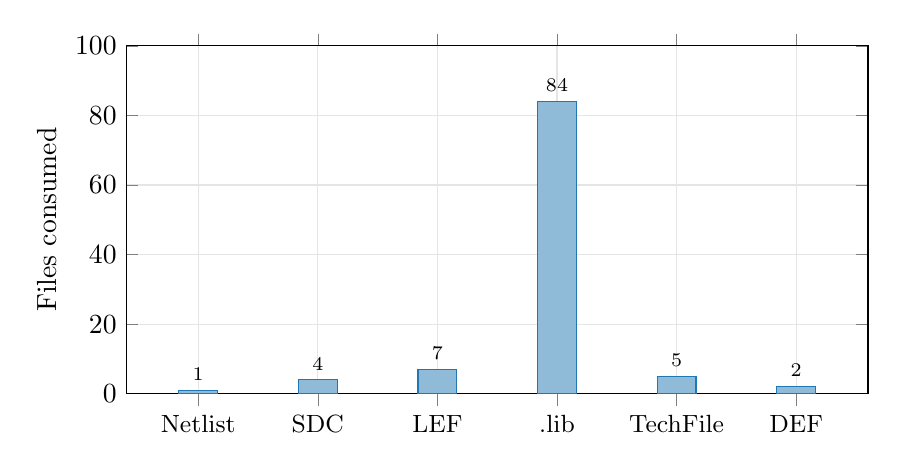
\begin{tikzpicture}
\begin{axis}[
  width=11cm, height=6cm,
  ybar, bar width=14pt,
  ymin=0, ymax=100,
  ylabel={Files consumed},
  symbolic x coords={Netlist, SDC, LEF, .lib, TechFile, DEF},
  xtick=data, x tick label style={font=\small},
  nodes near coords, nodes near coords style={font=\scriptsize},
  enlarge x limits=0.12,
  grid=major, grid style={black!10},
]
\addplot[fill=cKEY!50, draw=cKEY] coordinates {
  (Netlist,1) (SDC,4) (LEF,7) (.lib,84) (TechFile,5) (DEF,2)
};
\end{axis}
\end{tikzpicture}
\caption{Approximate file counts a single 7~nm SoC block consumes during PD setup. The .lib bar dominates because timing must be re-evaluated at every PVT and every cell-family combination.}
\label{fig:file-count}
\end{figure}

\begin{gut}
On a 7~nm design with 12 corners and 7 cell families, your bring-up script complains it cannot find \texttt{ss\_0p72v\_125c\_rvt.lib}. Which engine will fail first when you try to run anyway?
\gutans{The first stage that needs that specific worst-case slow corner for hold or max-cap analysis, typically CTS or post-route timing. The placer can often limp along on a single corner, but multi-corner optimization and signoff will refuse.}
\end{gut}

\section{Why the inputs are split, not merged}

\begin{sidebar}
A reasonable question: if all six artifacts feed one tool, why not merge them? The answer is \textbf{ownership and update cadence}. The foundry ships tech files once per process node revision (years). Cell libraries refresh on a quarterly basis. The architect rewrites SDC weekly during convergence. The netlist regenerates every nightly synthesis run. DEF flips on every floorplan iteration, sometimes hourly. A merged file would force the slowest-cadence team to gate the fastest-cadence team. The file boundary is a \textbf{social contract}, not a technical limit.

There is a second reason: format standards are owned by different bodies. LEF and DEF are Cadence-originated, .lib is Synopsys-originated, SDC is also Synopsys, the tech file is foundry-proprietary. The split survives because nobody can unify the standards bodies.
\end{sidebar}

\begin{pitfall}
The most common fresher mistake: assuming \texttt{.lib} and \texttt{LEF} are the same thing because both contain ``cell'' information. They are not. \textbf{.lib is timing only, LEF is geometry only.} A cell appears in both files under the same name, but the two views never overlap in content. If you cannot answer ``which file has the pin capacitance'' (\texttt{.lib}) versus ``which file has the pin location'' (\texttt{LEF}), the interviewer will know.
\end{pitfall}

\begin{pdnote}
\begin{itemize}[leftmargin=1.2em]
  \item \textbf{Arm PD intern lens.} Day one, you will be handed a block bring-up script that sources a netlist, an SDC, a LEF list, a .lib list, and a tech file. You will be expected to know which environment variable points to which file and which one to grep first when bring-up fails.
  \item \textbf{Foundry-flow PD engineer lens.} Production flows version-pin every input. A .lib refresh from the foundry triggers a full MMMC re-characterization. The flow's job is to detect input drift before signoff, not after.
  \item \textbf{VLSI interview lens.} The interviewer is not testing memorization. They are testing whether you understand that timing, geometry, intent, and parasitics are \textbf{orthogonal concerns} and that the file split mirrors the concern split. Answer in that frame and you stand out.
\end{itemize}
\end{pdnote}

\begin{checkpoint}
You can now name the six PD inputs, the question each answers, the engine that breaks without each, and the rough multiplier that makes a single .lib reference into 84 actual files. The rest of the book is one chapter per artifact.

\mnemonic{NSL-LTD: Netlist, SDC, LEF, Lib, Tech, DEF}
\end{checkpoint}

\chapter{The Netlist: A Wire-Level Blueprint}

\begin{tldr}
\begin{itemize}
  \item \textbf{Last chapter:} PD is a pipeline of engines, each demanding one irreplaceable input. \textbf{This chapter:} we crack open the first input (the netlist) and see the graph the rest of the flow walks across.
  \item A \textbf{netlist} is a textual graph of the design: \textbf{cell instances} as nodes, \textbf{nets} as edges, and \textbf{top-level ports} as the boundary.
  \item \textbf{Synthesis} converts RTL behavior into a netlist of library cells; the same RTL can be re-synthesized into a different technology and produce a different netlist.
  \item Every instance name in a \textbf{synthesized (gate-level) netlist} must resolve to a cell defined in the technology \texttt{.lib}, or the PD tool will throw a missing-reference error before floorplanning even begins.
\end{itemize}
\end{tldr}

\begin{hook}
Hand a physical design tool a million-line netlist and it sees one thing: a giant adjacency list of cells and the wires soldering them together. Strip away the comments, the module wrappers, the friendly signal names, and what is left is a circuit graph. That graph is the only thing the placer, the router, and the timing engine ever really look at. So what does this graph actually say?
\end{hook}

\section{What a Netlist Really Is}

A \textbf{netlist} is a connectivity description. It enumerates the \textbf{components} (cell instances) in the circuit and lists the \textbf{nodes} (nets) that those components share. A \textbf{net} is a single equipotential wire that touches two or more pins. A \textbf{port} is a wire that crosses the module boundary to the outside world.

That is the whole data structure. Three sets: instances, nets, ports. Every PD tool builds the same in-memory graph from whichever text format it was handed.

\begin{keyidea}
A netlist is a \textbf{graph of cell instances connected by nets}, with top-level ports as the only opening to the outside world; everything PD does (placement, routing, timing) operates on this graph.
\end{keyidea}

\section{The 4-Gate Example}

The lecture builds a tiny majority-style circuit with three AND gates feeding one OR gate. The structural picture looks like this.

\begin{figure}[h]
\centering
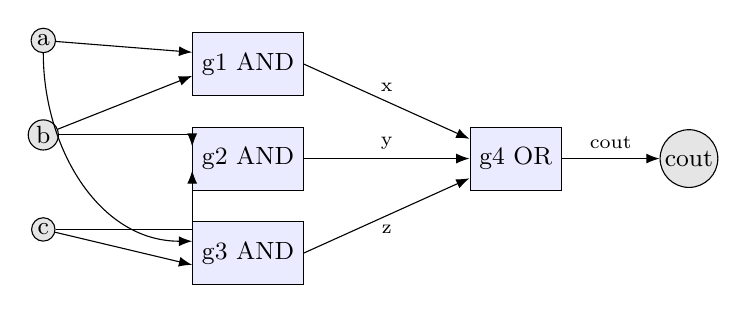
\begin{tikzpicture}[
  every node/.style={font=\small},
  gate/.style={draw, rectangle, minimum width=10mm, minimum height=8mm, fill=blue!8},
  port/.style={draw, circle, inner sep=1pt, fill=gray!20},
  node distance=8mm
]
  \node[port] (a) at (0,2.4) {a};
  \node[port] (b) at (0,1.2) {b};
  \node[port] (c) at (0,0)   {c};

  \node[gate] (g1) at (2.6,2.1) {g1 AND};
  \node[gate] (g2) at (2.6,0.9) {g2 AND};
  \node[gate] (g3) at (2.6,-0.3) {g3 AND};

  \node[gate] (g4) at (6.0,0.9) {g4 OR};
  \node[port] (cout) at (8.2,0.9) {cout};

  \draw[-Latex] (a)  -- ($(g1.west)+(0,0.15)$);
  \draw[-Latex] (b)  -- ($(g1.west)+(0,-0.15)$);

  \draw[-Latex] (b)  -| ($(g2.west)+(0,0.15)$);
  \draw[-Latex] (c)  -| ($(g2.west)+(0,-0.15)$);

  \draw[-Latex] (a)  to[out=-90,in=180] ($(g3.west)+(0,0.15)$);
  \draw[-Latex] (c)  -- ($(g3.west)+(0,-0.15)$);

  \draw[-Latex] (g1.east) -- node[above,font=\scriptsize] {x} ($(g4.west)+(0,0.25)$);
  \draw[-Latex] (g2.east) -- node[above,font=\scriptsize] {y} (g4.west);
  \draw[-Latex] (g3.east) -- node[below,font=\scriptsize] {z} ($(g4.west)+(0,-0.25)$);

  \draw[-Latex] (g4.east) -- node[above,font=\scriptsize] {cout} (cout);
\end{tikzpicture}
\caption{Structural view of the 4-gate example. Four instances (g1, g2, g3, g4), three internal nets (x, y, z), three input ports (a, b, c), one output port (cout).}
\label{fig:netlist-4gate}
\end{figure}

Count what the graph contains: \textbf{4 instances}, \textbf{3 internal nets}, \textbf{4 ports}. Every wire in the picture maps to exactly one entry in the netlist text.

\begin{hook}
Picture a \textbf{telephone switchboard} where each operator (cell instance) holds labeled cords (pins) and every cord plugs into a single colored wire bundle (net) running across the back panel. Lose one cord-to-bundle mapping and the call drops, which in silicon means the placer refuses to start.
\end{hook}

\section{The Verilog Form}

Here is what the four-gate circuit looks like as a technology-independent Verilog netlist.

\begin{lstlisting}[style=eda,caption={Technology-independent gate-level netlist for the 4-gate example.},label={lst:netlist-gen}]
module maj_block (a, b, c, cout);
  input  a, b, c;
  output cout;
  wire   x, y, z;

  and  g1 (x, a, b);
  and  g2 (y, b, c);
  and  g3 (z, a, c);
  or   g4 (cout, x, y, z);
endmodule
\end{lstlisting}

Read it as three blocks. The \textbf{header} declares ports. The \textbf{wire} statement names internal nets. The body \textbf{instantiates} cells, listing the output pin first and inputs after.

\begin{gut}
In Listing \ref{lst:netlist-gen}, how many \textbf{nets} does the design contain in total (count ports as nets too, since each is a wire crossing the boundary)?
\gutans{Seven: three input ports (a, b, c), one output port (cout), and three internal wires (x, y, z).}
\end{gut}

\section{Technology-Independent vs.\ Synthesized}

The lecture draws a sharp line at the end. The Verilog above uses generic \texttt{and} and \texttt{or} primitives. No PD tool can place those, because they have no area, no pin locations, no drive strength. That version is a \textbf{technology-independent netlist}: pure structure.

A \textbf{synthesized (gate-level) netlist} replaces every primitive with a \textbf{reference} to a real library cell, like \texttt{AND2\_X1} or \texttt{OR3\_X2} from a foundry standard-cell library.

\begin{figure}[h]
\centering
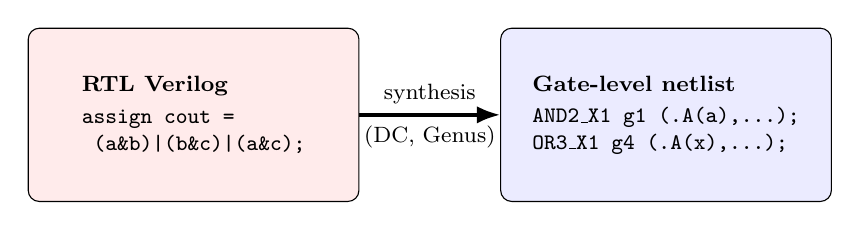
\begin{tikzpicture}[every node/.style={font=\footnotesize}, node distance=6mm]
  \node[draw, rounded corners, fill=red!8, minimum width=42mm, minimum height=22mm, align=left] (rtl) at (0,0)
    {\textbf{RTL Verilog}\\[2pt]
     \texttt{assign cout =}\\
     \texttt{ (a\&b)|(b\&c)|(a\&c);}};
  \node[draw, rounded corners, fill=blue!8, minimum width=42mm, minimum height=22mm, align=left] (gate) at (6.0,0)
    {\textbf{Gate-level netlist}\\[2pt]
     \texttt{AND2\_X1 g1 (.A(a),...);}\\
     \texttt{OR3\_X1  g4 (.A(x),...);}};
  \draw[-Latex, very thick] (rtl) -- node[above] {synthesis} node[below] {(DC, Genus)} (gate);
\end{tikzpicture}
\caption{Before/after: the same intent expressed as behavioral RTL (left) and as a synthesized gate-level netlist bound to library cells (right). PD only consumes the right-hand form.}
\label{fig:rtl-vs-gate}
\end{figure}

The mapping from RTL to gate-level is what the synthesis tool (Design Compiler, Genus, Yosys) does. Same RTL, different \texttt{.lib} target, different netlist. That is why one Verilog source survives a node shrink while the netlist gets thrown out and regenerated.

\begin{hook}
A \textbf{recipe} (RTL) survives moving to a new \textbf{kitchen} (foundry), but the \textbf{ingredient list with brand names} (netlist) gets rewritten every time, and serving the wrong brand (a cell not in the \texttt{.lib}) ruins the whole dish (the PD database refuses to load).
\end{hook}

\begin{pausebox}
Pause. Before reading on, sketch what would happen if your synthesis target was a 7\,nm \texttt{.lib} but you handed PD the netlist synthesized against the 28\,nm library. Where in the flow does the failure show up, and what does the error message complain about?
\end{pausebox}

\section{Why Cell Names Matter (Chapter 9 Foreshadow)}

Every reference name in the synthesized netlist (e.g., \texttt{NAND2\_X2}) is a string lookup into the technology \texttt{.lib}. If the netlist says \texttt{NAND2\_X2} but the library only defines \texttt{NAND2X2} (no underscore), the PD tool reports an unresolved reference and refuses to elaborate the design.

This is why you cannot mix-and-match. The netlist, the \texttt{.lib}, and the LEF (Chapter 9) must all agree on cell names down to the character. We will see in the next chapter why the \texttt{.lib} is the source of truth for those names.

\section{Worked Example: Counting What PD Sees}

\textbf{Problem.} For the netlist in Listing \ref{lst:netlist-gen}, compute the instance count, the net count, and the average net degree (pins per net).

\move{1} \textbf{Instances.} g1, g2, g3, g4 \(\Rightarrow\) \(N_{\text{inst}} = 4\).

\move{2} \textbf{Nets.} Internal: \{x, y, z\}. Port nets: \{a, b, c, cout\}. Total \(N_{\text{net}} = 7\).

\move{3} \textbf{Pin count per net.} Each input port drives certain gates:
\begin{itemize}
  \item \texttt{a}: 1 port + g1.A + g3.A \(\Rightarrow\) 3 pins
  \item \texttt{b}: 1 port + g1.B + g2.A \(\Rightarrow\) 3 pins
  \item \texttt{c}: 1 port + g2.B + g3.B \(\Rightarrow\) 3 pins
  \item \texttt{x}: g1.Z + g4.A \(\Rightarrow\) 2 pins
  \item \texttt{y}: g2.Z + g4.B \(\Rightarrow\) 2 pins
  \item \texttt{z}: g3.Z + g4.C \(\Rightarrow\) 2 pins
  \item \texttt{cout}: g4.Z + 1 port \(\Rightarrow\) 2 pins
\end{itemize}

\move{4} \textbf{Average degree.} Total pins \(= 3+3+3+2+2+2+2 = 17\). Average pins/net \(= 17/7 \approx 2.43\).

\move{5} \textbf{Scaling intuition.} Real SoCs run roughly 1 net per instance. For a 1\,M-instance block, expect on the order of \textbf{1\,M nets}. Each one becomes a routing problem.

\begin{figure}[h]
\centering
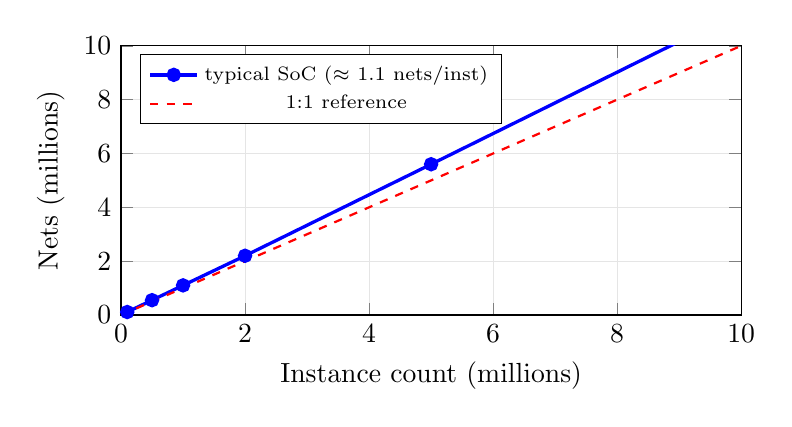
\begin{tikzpicture}
\begin{axis}[
  width=0.78\linewidth, height=5cm,
  xlabel={Instance count (millions)},
  ylabel={Nets (millions)},
  xmin=0, xmax=10, ymin=0, ymax=10,
  grid=both, grid style={gray!20},
  legend pos=north west, legend style={font=\scriptsize}
]
\addplot[blue, very thick, mark=*] coordinates {(0.1,0.11)(0.5,0.55)(1,1.1)(2,2.2)(5,5.6)(10,11.3)};
\addlegendentry{typical SoC ($\approx$ 1.1 nets/inst)}
\addplot[red, dashed, thick] coordinates {(0,0)(10,10)};
\addlegendentry{1:1 reference}
\end{axis}
\end{tikzpicture}
\caption{Net count vs.\ instance count for synthesized blocks. The slope sits slightly above 1 because high-fanout nets (clock, reset, scan-enable) push the average up.}
\label{fig:net-scaling}
\end{figure}

\begin{gut}
For a block with 250{,}000 instances, what is a reasonable first-cut estimate of the net count, and what single signal probably skews that number upward?
\gutans{Around 275{,}000 nets (1.1$\times$ rule). The \textbf{clock net} typically touches every flop, but it gets split into a tree by CTS so the raw netlist still shows it as one giant net.}
\end{gut}

\begin{pitfall}
\textbf{Common netlist misconceptions.}
\begin{itemize}
  \item \textbf{Behavioral vs.\ structural.} A file with \texttt{always} blocks or \texttt{assign} expressions is \emph{not} a netlist PD can consume. PD wants pure structural Verilog: instances and connections only.
  \item \textbf{Blackboxes.} An instance whose module body is not in the netlist (memories, hard macros, IP blocks) is a \textbf{blackbox}. PD still needs its physical view (LEF) and timing view (\texttt{.lib}); otherwise it cannot place or time around it.
  \item \textbf{Cell name mismatch.} \texttt{INVX1} in the netlist will not bind to \texttt{INV\_X1} in the \texttt{.lib}. Spelling, case, and underscores all matter.
  \item \textbf{Non-uniquified hierarchical netlists.} If the same module is instantiated under two parents that need different constraints (say, one on a critical 1\,GHz datapath, the other in scan-only logic), synthesis must \textbf{uniquify} by renaming each instance to a distinct module. A non-uniquified netlist applies one set of timing budgets to both, and the failing endpoint shows up only at signoff, after a week of PD work.
  \item \textbf{Physical-only cells without \texttt{.lib} entries.} Tap cells, end-caps, decaps, and ECO fillers live in the netlist (or get inserted post-synthesis) but have no timing arcs in \texttt{.lib}. PD tools handle this gracefully; STA-only flows can throw confusing missing-pin errors if the engineer forgot to mark them as physical-only.
\end{itemize}
\end{pitfall}

\begin{sidebar}
\textbf{Hierarchical vs.\ flat netlists.} A hierarchical netlist preserves module boundaries (\texttt{cpu/alu/adder/g1}); a flat netlist dissolves them so every leaf instance lives at the top (\texttt{cpu\_alu\_adder\_g1}). Hierarchical is easier for humans and faster to elaborate; flat gives the optimizer freedom to retime and resize across former boundaries. Most modern flows stay hierarchical at top and flatten selectively inside each block.

\textbf{EDIF.} Older flows and some FPGA tools exchange netlists in \textbf{EDIF} (Electronic Design Interchange Format), a Lisp-like S-expression syntax. The information is identical; the grammar is just uglier. ASIC PD today is overwhelmingly Verilog.
\end{sidebar}

\begin{pdnote}
\textbf{Why PD cares.}
\begin{itemize}
  \item \textbf{ARM PD internship lens:} the first thing you do on day one is load a synthesized \texttt{.v} into Innovus or ICC2 and check that every reference resolves against the loaded \texttt{.lib}/LEF; unresolved references are the most common ``my flow won't start'' ticket.
  \item \textbf{Generic foundry-flow PD engineer lens:} the netlist drives \textbf{instance count budgeting} (placement density), \textbf{net count budgeting} (routing congestion), and \textbf{port count budgeting} (pin planning at block boundaries); all three pop out of a 30-second \texttt{report\_design} run.
  \item \textbf{VLSI interview lens:} expect ``what is the difference between a behavioral and a structural netlist?'' and ``which inputs does PD need before placement?''; the netlist is always one of the three answers (netlist, \texttt{.lib}, LEF).
\end{itemize}
\end{pdnote}

\begin{checkpoint}
You should now be able to: (1) define a netlist as an instance/net/port graph, (2) distinguish a technology-independent netlist from a synthesized one, (3) read a small Verilog gate-level netlist and count instances and nets, and (4) explain why every reference in the netlist must match a cell in the \texttt{.lib}.

\mnemonic{INP: Instances, Nets, Ports}
\end{checkpoint}

\chapter{The Timing Library (.lib): How Cells Tell Time}

\begin{tldr}
\begin{itemize}[leftmargin=*]
  \item \textbf{Last chapter:} a netlist is just a graph of instances, nets, and ports. \textbf{This chapter:} we feed that graph to the timing engine, which only knows what each cell does because the \texttt{.lib} tells it.
  \item A \textbf{.lib} is the Liberty-format file that tells every EDA tool how each standard cell behaves: its pins, function, timing arcs, power, and leakage.
  \item Timing inside a .lib is stored as \textbf{NLDM lookup tables} indexed by \textbf{input slew} and \textbf{output load}; the tool reads the table and \textbf{bilinearly interpolates} when your operating point falls between grid samples.
  \item \textbf{CCS} and \textbf{ECSM} add a third axis (time-varying current) to model Miller capacitance accurately at sub-130\,nm nodes, at the cost of much larger library files.
  \item Foundries deliver one .lib per \textbf{PVT corner} (slow-slow worst case, typical, fast-fast best case); a real flow loads many of them under \textbf{MMMC} so STA can sign off across all corners simultaneously.
  \item Tools compile .lib into a binary \textbf{.db} (Synopsys) for fast ingestion, but engineers always debug against the human-readable .lib.
\end{itemize}
\end{tldr}

\section*{Why this chapter exists}

You hand the place-and-route tool a netlist that says \texttt{INVX1 U7 (.A(n42), .Y(n43));}. The tool stares back and asks a question you cannot answer from the netlist alone: \emph{how long does it take for a transition on n42 to appear on n43?} That number is not in the Verilog. It is not in the library exchange format. It lives in exactly one place, and that place is the timing library. Without it, no static timing analysis runs, no gate sizing happens, no clock tree gets built, and no chip taped out.

\textbf{This chapter unpacks what is actually inside that file.} We will look at a real NLDM lookup table, watch a tool interpolate a delay value step by step, and then see where NLDM breaks down and CCS takes over.

\section{The Two Axes of Cell Delay}

A standard cell's delay is not a constant. It depends on \textbf{how sharp the incoming edge is} (input slew, or \texttt{tran}) and \textbf{how much capacitance the output is driving} (output load, or \texttt{cap}). A slow input edge stretches the delay; a heavy output load stretches it more. Every other gate-level timing question reduces to those two knobs.

The Liberty file captures this by storing a 2D \textbf{lookup table} per timing arc per cell. Rows are discrete input-slew values. Columns are discrete output-load values. Each cell holds a delay (and a separate table holds output slew). When the tool needs a point that is not on the grid, it interpolates.

\subsection*{Figure 1: NLDM delay surface for an INVX1 cell}

\begin{figure}[h]
\centering
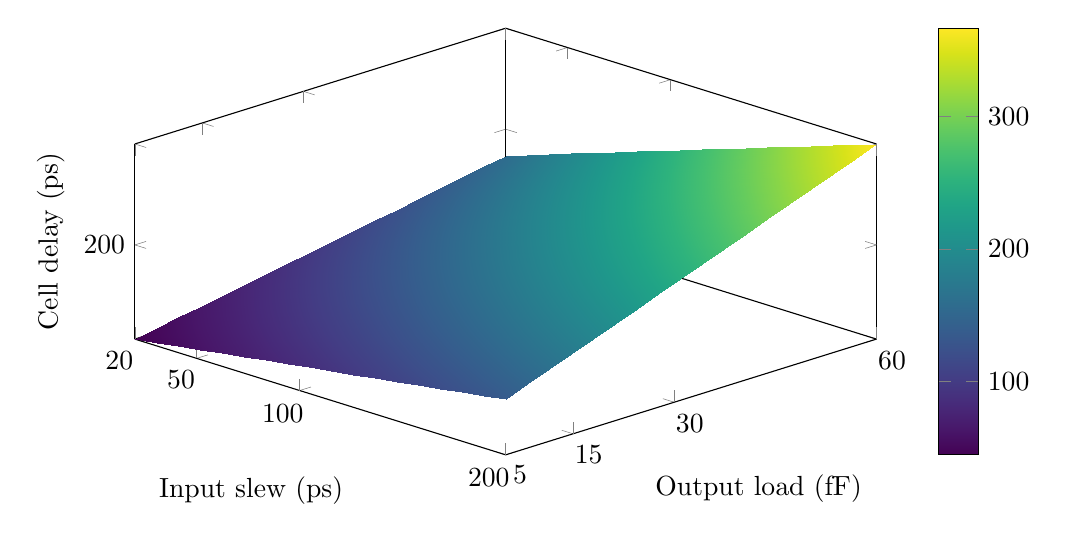
\begin{tikzpicture}
  \begin{axis}[
    width=11cm, height=7cm,
    view={45}{40},
    xlabel={Input slew (ps)},
    ylabel={Output load (fF)},
    zlabel={Cell delay (ps)},
    colormap/viridis, colorbar,
    xtick={20,50,100,200}, ytick={5,15,30,60},
    enlargelimits=false,
  ]
    \addplot3[surf, shader=interp, samples=18, domain=20:200, y domain=5:60]
      {25 + 0.45*x + 1.8*y + 0.012*x*y};
  \end{axis}
\end{tikzpicture}
\caption{NLDM delay surface for a representative INVX1 cell. Delay grows roughly linearly with each axis and faster along the diagonal because the slew and load effects multiply. Real .lib tables sample this surface at \textbf{3 to 7 grid points per axis}.}
\end{figure}

\begin{hook}
\textbf{Hook 1.} \textbf{The fork pierces the steak slowly when the steak is cold.} A cold steak is a heavy load; a dull fork is a slow slew. Both make the bite take longer. Stakes: order the wrong cell drive strength and your hold-time margin evaporates before you can re-spin.
\end{hook}

\begin{hook}
\textbf{Hook 2.} \textbf{The librarian stamps every book at three temperatures.} The .lib is the stamp catalog; the librarian is the foundry; the temperatures are PVT corners. Skip a corner and a chip ships that fails in the Arizona heat. Stakes: an entire wafer lot scrapped.
\end{hook}

\begin{gut}
\textbf{Gut check 1.} If you double the output load but keep input slew fixed, what happens to cell delay in an NLDM model?
\gutans{It grows, but not linearly in general. The lookup table captures whatever curvature the SPICE characterization measured. For an INVX1 on a typical 28\,nm node, doubling load from 15\,fF to 30\,fF might raise delay by roughly 60 to 80 percent.}
\end{gut}

\begin{gut}
\textbf{Gut check 2.} Why does the .lib store \emph{two} tables (rise and fall) per timing arc instead of one?
\gutans{NMOS and PMOS have different mobilities. The pull-down path through NMOS is usually faster than the pull-up through PMOS, so rise and fall delays differ. The tool needs both to compute setup and hold against the correct edge.}
\end{gut}

\begin{pausebox}
So far: a .lib is the file that tells the tool how a cell delays a signal, the delay depends on input slew and output load, and the data is stored as a 2D table per arc per cell. Next: we read a real Liberty snippet and then do the arithmetic the tool does.
\end{pausebox}

\begin{keyidea}
A timing library is a \textbf{characterized lookup of cell behavior across PVT corners}. The NLDM model boils every cell's delay down to a 2D table indexed by input slew and output load, and the tool interpolates between grid points whenever your operating condition falls in between.
\end{keyidea}

\section{What a Liberty File Actually Looks Like}

\subsection*{Figure 2: A real Liberty timing block for an inverter}

\begin{lstlisting}[style=eda, language=, caption={Excerpt of an INVX1 cell in Liberty format. The \texttt{lu\_table\_template} (defined once at the top of the .lib) declares the index variables; each \texttt{cell\_rise} / \texttt{cell\_fall} group fills in the delay surface for one timing arc.}]
library (tsmc28_tt_0p9v_25c) {
  time_unit              : "1ns";
  capacitive_load_unit (1, ff);
  voltage_unit           : "1V";
  nom_voltage            : 0.90;
  nom_temperature        : 25.0;

  lu_table_template (delay_template_3x3) {
    variable_1 : input_net_transition;
    variable_2 : total_output_net_capacitance;
    index_1 ("20.0, 100.0, 200.0");   /* ps */
    index_2 ("5.0,  15.0,  30.0");    /* fF */
  }

  cell (INVX1) {
    area : 1.764;
    pin (A) { direction : input;  capacitance : 1.42; }
    pin (Y) {
      direction : output;
      function  : "!A";
      max_capacitance : 60.0;
      timing () {
        related_pin   : "A";
        timing_sense  : negative_unate;
        cell_rise (delay_template_3x3) {
          values ( "0.045, 0.062, 0.091", \
                   "0.071, 0.094, 0.135", \
                   "0.108, 0.142, 0.198" );
        }
        cell_fall (delay_template_3x3) {
          values ( "0.038, 0.054, 0.080", \
                   "0.061, 0.083, 0.121", \
                   "0.094, 0.127, 0.178" );
        }
      }
    }
  }
}
\end{lstlisting}

Two things deserve attention in that listing. First, the \textbf{units block at the top} sets the scale for every number below: delays are in \texttt{ns}, capacitances in \texttt{fF}. Misreading the unit is the single most common .lib bug junior engineers commit. Second, the \textbf{values} array is row-major, with rows indexed by \texttt{index\_1} (input slew) and columns by \texttt{index\_2} (output load).

\section{Worked Example: Bilinear Interpolation by Hand}

Let us take the \texttt{cell\_rise} table from the listing above and ask: what is the cell delay if the input slew is \textbf{50\,ps} and the output load is \textbf{15\,fF}? The exact load (15\,fF) sits on the grid, but the slew (50\,ps) falls between 20\,ps and 100\,ps, so we have to interpolate along one axis.

\textbf{Step 1: locate the bracketing grid points.} Slew 50\,ps lies between \texttt{index\_1[0]=20} and \texttt{index\_1[1]=100}. Load 15\,fF is exactly \texttt{index\_2[1]=15}.

\textbf{Step 2: pull the four corner delays.} Because load sits on the grid, only two corners matter:
\[
D(20\,\text{ps},\,15\,\text{fF}) = 0.062\,\text{ns}, \qquad D(100\,\text{ps},\,15\,\text{fF}) = 0.094\,\text{ns}.
\]

\textbf{Step 3: compute the slew fraction.}
\[
\alpha = \frac{50 - 20}{100 - 20} = \frac{30}{80} = 0.375.
\]

\textbf{Step 4: linearly blend.}
\[
D_{\text{interp}} = (1 - 0.375)\cdot 0.062 + 0.375 \cdot 0.094 = 0.625 \cdot 0.062 + 0.375 \cdot 0.094.
\]
\[
D_{\text{interp}} = 0.03875 + 0.03525 = 0.0740\,\text{ns} = \mathbf{74.0\,ps}.
\]

So the tool reports a rise delay of \textbf{74\,ps} for this INVX1 under those conditions. Now let us do the harder case where \emph{both} axes are off-grid: slew 50\,ps, load 22\,fF.

\move{1} Pull all four corners:
\[
\begin{aligned}
D_{00} &= D(20, 15) = 0.062, & D_{01} &= D(20, 30) = 0.091,\\
D_{10} &= D(100, 15) = 0.094, & D_{11} &= D(100, 30) = 0.135.
\end{aligned}
\]

\move{2} Compute fractions on each axis:
\[
\alpha = \tfrac{50-20}{100-20} = 0.375, \qquad \beta = \tfrac{22-15}{30-15} = \tfrac{7}{15} = 0.4667.
\]

\move{3} Interpolate along load at each slew value:
\[
D(20, 22) = (1-0.4667)\cdot 0.062 + 0.4667 \cdot 0.091 = 0.0331 + 0.0425 = 0.0756.
\]
\[
D(100, 22) = (1-0.4667)\cdot 0.094 + 0.4667 \cdot 0.135 = 0.0501 + 0.0630 = 0.1131.
\]

\move{4} Interpolate the two intermediate values along slew:
\[
D = (1-0.375)\cdot 0.0756 + 0.375 \cdot 0.1131 = 0.0473 + 0.0424 = \mathbf{0.0897\,\text{ns}} \approx \mathbf{90\,ps}.
\]

\move{5} Generalize to the abstract \textbf{bilinear interpolation formula}:
\[
D(s, c) = (1-\alpha)(1-\beta)\,D_{00} + \alpha(1-\beta)\,D_{10} + (1-\alpha)\beta\,D_{01} + \alpha\beta\,D_{11}
\]
where \(\alpha\) is the fractional position along input slew and \(\beta\) is the fractional position along output load. The hand arithmetic above is exactly this formula, executed in two passes.

\section{Setup, Hold, and the Other Tables}

NLDM does more than store cell delays. Every sequential cell (flip-flops, latches) carries additional 2D tables that encode timing checks: a \textbf{setup} table indexed by data-slew and clock-slew, and a \textbf{hold} table with the same axes. The tool reads these to determine whether captured data is stable around the active clock edge. There are also \textbf{recovery} and \textbf{removal} tables for asynchronous pins, and \textbf{output transition} tables that propagate the slew downstream so the next gate's delay table can be looked up correctly.

\begin{pitfall}
\textbf{Watch Out.}
\begin{itemize}[leftmargin=*]
  \item \textbf{Units are not universal.} One foundry's .lib uses \texttt{1ns} and \texttt{pF}; another uses \texttt{1ps} and \texttt{fF}. Mixing tools that disagree on the units block produces silent errors of 1000x.
  \item \textbf{NLDM is not CCS.} Reading a .lib that claims CCS support but only filling in NLDM tables gives you NLDM accuracy with CCS file size. Verify by grepping for \texttt{output\_current\_rise}.
  \item \textbf{Hold tables are not setup tables.} A common bug: copying setup characterization data into the hold slot. Setup and hold have opposite signs and different reference edges.
  \item \textbf{PVT corners are not interchangeable.} The slow-slow (\textbf{WC}) .lib is for setup analysis; the fast-fast (\textbf{BC}) .lib is for hold. Loading only the typical (TC) corner will sign off a chip that fails silicon.
\end{itemize}
\end{pitfall}

\section{Why CCS Exists (and Why NLDM Quietly Lies at 7nm)}

NLDM stores \textbf{one delay number} per (input slew, output load) grid point. That model rests on three assumptions, and every single one of them gets shakier as nodes shrink.

\textbf{Assumption 1: the output load is a fixed lumped capacitor.} It is not. Gate-to-drain coupling capacitance (the \textbf{Miller capacitance}) at the receiver gets multiplied by $(1 + A_v)$ where $A_v$ is the receiver's small-signal gain during the transition. In a fast switching transition the effective load the driver feels is meaningfully larger than the static fanout capacitance the .lib was characterized against.

\textbf{Assumption 2: the receiver's input pin capacitance is constant.} It is not. PMOS and NMOS gate capacitance is voltage-dependent: a gate in cutoff presents less capacitance than the same gate in saturation. As the input ramps, the load looks different at 30\% Vdd than at 70\% Vdd. NLDM averages this and ships one number per pin. CCS stores the nonlinearity.

\textbf{Assumption 3: only the slew (20\%-to-80\% or similar) matters, not the waveform shape.} At 130\,nm a slew was a clean, near-linear ramp. At 7\,nm the upstream driver's output is non-monotonic enough that two transitions with the same 20-80 slew can produce \textbf{different downstream delays}. NLDM cannot see this. CCS can, because it propagates the actual current waveform.

\begin{keyidea}
CCS replaces NLDM's single delay number with a \textbf{time-varying output current waveform per (slew, load) grid point}, so the next stage convolves \emph{actual current shape} into its own response instead of inheriting a slew-only summary.
\end{keyidea}

\paragraph{Worked example: when NLDM and CCS diverge.} A buffer drives a fanout-of-4 load. NLDM says: static load = 4 input gates $\times$ 1.0\,fF = 4.0\,fF, look up (slew = 50 ps, load = 4 fF) in the table, get \textbf{delay = 32 ps}. CCS sees that the receiver's effective Miller-multiplied capacitance during the transition is closer to $4.0 \times 1.4 = 5.6$\,fF, AND that the receiver pin cap rises by ~20\% as the input crosses the switching threshold. The CCS-computed delay is \textbf{closer to 42 ps}. \textbf{A 30\% error on a single stage, compounded over a 15-stage path, is the difference between meeting timing and missing it by 100\,ps.}

\textbf{ECSM} (Cadence) encodes the same physics with a voltage-vs-time waveform instead of current-vs-time. Same intent, different storage. Innovus consumes ECSM natively; PrimeTime consumes CCS. Foundries ship both.

\textbf{File size cost.} A CCS .lib is roughly 5 to 10x the size of the equivalent NLDM library because every (slew, load) entry now stores a sampled current waveform (typically 20 time points) instead of one delay scalar. This is why the .db (binary compiled .lib) matters: loading 200 CCS views as ASCII text would burn an hour on Liberty parsing alone.

\begin{sidebar}
\textbf{Why MMMC makes this worse.} CCS file size multiplied by MMMC view count is what actually fills your scratch disk. A 5\,nm block with 200 .lib views, each in CCS form at ~80\,MB, lands at ~16\,GB of library data per run. The binary .db form compresses this maybe 3x. \textbf{This is why the LIBPATH variable in Innovus matters and why corrupted .db caches eat days.}
\end{sidebar}

\begin{pdnote}
\begin{itemize}[leftmargin=*]
  \item \textbf{Arm internship lens.} When a designer hands you a failing path, the first reflex is to open the .lib for the offending cell and confirm its drive strength, max-cap, and the actual delay numbers at the path's slew and load. Half the bugs assigned to junior PD engineers turn out to be a misloaded corner library.
  \item \textbf{Foundry-flow PD engineer lens.} You will routinely load \textbf{8 to 32 libraries} per run under MMMC: WC, TC, BC across two voltage rails and three temperatures, times functional mode (sleep, active, scan). Knowing which corner pessimizes setup vs hold determines which library a slack violation belongs to and where the fix has to land.
  \item \textbf{VLSI interview lens.} Expect \emph{"walk me through what's inside a .lib file"} and \emph{"why CCS over NLDM at advanced nodes?"} as warm-up questions. The strong answer names the units block, the lookup template, the timing arc with related\_pin and timing\_sense, and finishes with Miller capacitance and receiver-pin modeling as the CCS justification.
\end{itemize}
\end{pdnote}

\begin{checkpoint}
You can now (1) name the four things a .lib stores per cell (pins, function, timing arcs, power), (2) read an NLDM lookup table and bilinearly interpolate a delay by hand, (3) explain why CCS exists and what it adds, and (4) defend why a real flow loads many .lib files under MMMC rather than just one.

\mnemonic{Slew in, load out, table in the middle, corner on the side.}
\end{checkpoint}

\chapter{The LEF File: Physical Abstraction of Cells and Layers}

\begin{tldr}
\begin{itemize}[leftmargin=*,nosep]
  \item \textbf{Last chapter:} the \texttt{.lib} stored cell behavior as NLDM lookup tables across PVT. \textbf{This chapter:} the LEF stores the same cell's physical footprint, so the placer can put it somewhere legal without ever opening the GDS.
  \item The \textbf{LEF (Library Exchange Format)} file gives the placer and router the \textbf{physical view} of every cell that the timing \texttt{.lib} characterized: bounding box, pin shapes, blockages, and which layer each pin lives on.
  \item LEF comes in two flavors that get shipped separately: a \textbf{technology LEF} (one per process node, describing metal layers, vias, and design rules) and a \textbf{cell LEF} (one per standard cell library, describing each \texttt{MACRO}).
  \item LEF deliberately throws away the transistor-level GDS. The placer never sees diffusion or poly. It sees rectangles on metal layers and a placement \texttt{SITE} grid. GDS only re-enters the flow at LVS and tape-out.
  \item Inside a \texttt{MACRO}: \texttt{SIZE} (width $\times$ height), \texttt{SYMMETRY}, \texttt{SITE}, one \texttt{PIN} block per logical pin (with \texttt{PORT} geometries on specific \texttt{LAYER}s), and \texttt{OBS} blockages that the router must avoid.
\end{itemize}
\end{tldr}

\section{Why the placer is blind to your beautiful layout}

Your standard cell layout is a stick diagram with diffusion, poly, contacts, and three or four metal layers. It is gorgeous. The placer does not care. When the placer drops an \texttt{INV\_X1} into a row, it is moving a small \textbf{rectangle of width $W$ and height $H$}, snapping its origin to a \texttt{SITE} on a row, and asking one question: \emph{do the pin shapes on M1 line up with a routing track?}

Everything else (the FET widths, the poly pitch, the well taps) is \textbf{stripped out} before the cell ever reaches P\&R. The file that does the stripping is the LEF.

\begin{figure}[h]
\centering
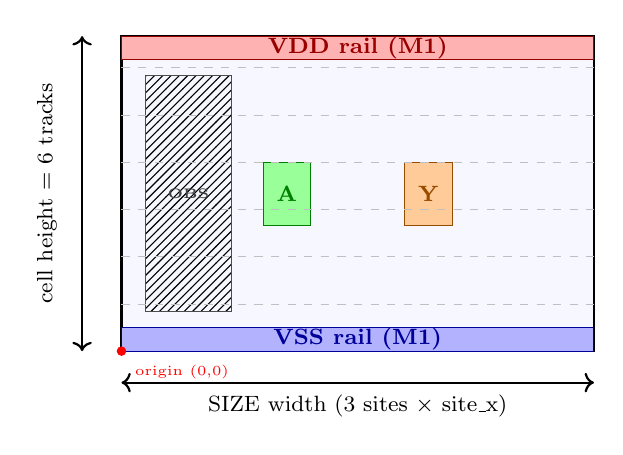
\begin{tikzpicture}[scale=1.0, every node/.style={font=\footnotesize}]
  % Cell boundary
  \draw[thick, fill=blue!3] (0,0) rectangle (6,4);
  % VDD rail (top)
  \draw[fill=red!30, draw=red!60!black] (0,3.7) rectangle (6,4.0);
  \node[red!60!black, font=\bfseries\footnotesize] at (3,3.85) {VDD rail (M1)};
  % VSS rail (bottom)
  \draw[fill=blue!30, draw=blue!60!black] (0,0) rectangle (6,0.3);
  \node[blue!60!black, font=\bfseries\footnotesize] at (3,0.15) {VSS rail (M1)};
  % Input pin A on M1
  \draw[fill=green!40, draw=green!50!black] (1.8,1.6) rectangle (2.4,2.4);
  \node[green!50!black] at (2.1,2.0) {\textbf{A}};
  % Output pin Y on M1
  \draw[fill=orange!40, draw=orange!60!black] (3.6,1.6) rectangle (4.2,2.4);
  \node[orange!60!black] at (3.9,2.0) {\textbf{Y}};
  % OBS region
  \draw[fill=gray!30, draw=gray!60!black, pattern=north east lines] (0.3,0.5) rectangle (1.4,3.5);
  \node[gray!50!black, font=\tiny] at (0.85,2.0) {\textbf{OBS}};
  % Routing tracks (dashed)
  \foreach \y in {0.6,1.2,1.8,2.4,3.0,3.6} {
    \draw[dashed, gray!50, very thin] (0,\y) -- (6,\y);
  }
  % Cell height bracket
  \draw[<->, thick] (-0.5,0) -- (-0.5,4);
  \node[rotate=90, anchor=south] at (-0.7,2) {cell height = 6 tracks};
  % Width
  \draw[<->, thick] (0,-0.4) -- (6,-0.4);
  \node at (3,-0.7) {SIZE width (3 sites $\times$ site\_x)};
  % Origin marker
  \filldraw[red] (0,0) circle (1.5pt);
  \node[red, anchor=north west, font=\tiny] at (0.05,-0.05) {origin (0,0)};
\end{tikzpicture}
\caption{Abstract physical view of an \texttt{INV\_X1} as seen through the LEF. The placer sees this rectangle, the VDD/VSS rails, the M1 pin shapes for \texttt{A} and \texttt{Y}, and the \texttt{OBS} blockage. It never sees the transistors underneath.}
\label{fig:inv-abstract}
\end{figure}

\begin{hook}
\textbf{LEF is the placer's passport photo.} The cell's full GDS face stays home; only the \textbf{rectangle, the pins, and the rails} travel through P\&R. If the passport photo is wrong, the cell still gets stopped at the border (DRC).
\end{hook}

\begin{hook}
\textbf{Tech-LEF paints the streets; cell-LEF parks the cars.} The tech-LEF declares which metal layers exist, their pitch, and their direction. The cell-LEF tells the tool where each cell parks on those streets. Mismatched grids mean the cars do not fit between the curbs.
\end{hook}

\begin{gut}
A placer is dropping an \texttt{INV\_X1} into a row. Which of these does it read from the LEF, and which from the \texttt{.lib}? (a) cell delay vs.\ load, (b) cell width in microns, (c) pin \texttt{A} input capacitance, (d) which metal layer pin \texttt{A} sits on.
\gutans{LEF: (b) and (d). Timing \texttt{.lib}: (a) and (c). LEF is physical only. The .lib is electrical only. They share cell names so the tool can join the two views.}
\end{gut}

\begin{gut}
You open a cell LEF and see \texttt{SIZE 0.6 BY 1.2}. Where does the unit (microns vs.\ database units) come from?
\gutans{The technology LEF, via the \texttt{UNITS} section (typically \texttt{DATABASE MICRONS 1000} or similar). The cell LEF inherits the unit; it does not redeclare it.}
\end{gut}

\begin{pausebox}
So far: LEF abstracts the physical view, ships in two pieces (tech + cell), and intentionally hides the GDS. Next we nail down the one sentence that justifies everything else in this chapter.
\end{pausebox}

\begin{keyidea}
The LEF is the \textbf{contract between the cell library and the placer/router}: it promises that a cell will occupy exactly this footprint, expose pins on exactly these layers at exactly these coordinates, and block routing in exactly these regions, so the tool can resolve placement and routing \textbf{without ever opening the GDS}.
\end{keyidea}

\section{Anatomy of a MACRO block}

A cell LEF is a stack of \texttt{MACRO} blocks. Each block declares the cell name, its bounding box, what kind of cell it is (\texttt{CLASS CORE}, \texttt{PAD}, \texttt{BLOCK}, etc.), which placement site it snaps to, and then one \texttt{PIN} sub-block per logical pin plus an \texttt{OBS} sub-block for blockages.

\begin{figure}[h]
\centering
\begin{lstlisting}[style=eda, basicstyle=\ttfamily\footnotesize, frame=single]
MACRO INV_X1
  CLASS CORE ;
  ORIGIN 0 0 ;
  SIZE 0.6 BY 1.2 ;
  SYMMETRY X Y ;
  SITE CoreSite ;

  PIN A
    DIRECTION INPUT ;
    USE SIGNAL ;
    ANTENNAGATEAREA 0.14 ;
    PORT
      LAYER M1 ;
        RECT 0.18 0.40 0.24 0.80 ;
    END
  END A

  PIN Y
    DIRECTION OUTPUT ;
    USE SIGNAL ;
    PORT
      LAYER M1 ;
        RECT 0.36 0.40 0.42 0.80 ;
    END
  END Y

  PIN VDD
    DIRECTION INOUT ; USE POWER ;
    PORT LAYER M1 ; RECT 0.00 1.13 0.60 1.20 ; END
  END VDD

  PIN VSS
    DIRECTION INOUT ; USE GROUND ;
    PORT LAYER M1 ; RECT 0.00 0.00 0.60 0.07 ; END
  END VSS

  OBS
    LAYER M1 ; RECT 0.05 0.10 0.14 1.10 ;
  END
END INV_X1
\end{lstlisting}
\caption{A cell-LEF \texttt{MACRO} excerpt for an \texttt{INV\_X1}. Coordinates are in microns (set by the tech LEF). Pins \texttt{A} and \texttt{Y} expose M1 rectangles; \texttt{VDD}/\texttt{VSS} stripe the top and bottom; \texttt{OBS} blocks a region of M1 from the router.}
\label{fig:lef-listing}
\end{figure}

A few items deserve a closer look. \texttt{SYMMETRY X Y} tells the placer it may mirror this cell about either axis (commonly used to flip every other row so VDD/VSS rails abut). \texttt{SITE CoreSite} ties the cell to a placement site defined in the tech-LEF; the cell's width must be an integer multiple of the site width. \texttt{OBS} is a router-only directive that says \emph{do not route here}, typically used to hide internal M1 jumpers from the routing tool.

\section{Worked example: site arithmetic for an INV\_X1}

\move{1}
Given: cell \texttt{SIZE 0.6 BY 1.2} (microns). Tech-LEF declares \texttt{SITE CoreSite SIZE 0.2 BY 1.2}. We want: how many sites the cell occupies horizontally, its area, and whether it aligns to the row grid.


\move{2}
Sites occupied horizontally: $N_{\text{sites}} = \dfrac{W_{\text{cell}}}{W_{\text{site}}} = \dfrac{0.6}{0.2} = 3$ sites. The cell consumes a contiguous run of \textbf{three placement sites}.


\move{3}
Row alignment: row height is the site height $= 1.2\,\si{\micro\meter}$, and the cell height is also $1.2\,\si{\micro\meter}$. Match. The cell fits exactly in one row, with its VDD pin on the top edge and VSS on the bottom.


\move{4}
Cell area: $A = W \times H = 0.6 \times 1.2 = 0.72\,\si{\micro\meter\squared}$. This is what the placer reports for utilization accounting, not the active silicon area.


\move{5}
Sanity check: if a designer had written \texttt{SIZE 0.55 BY 1.2}, then $0.55 / 0.2 = 2.75$ sites. The placer would either reject the macro at library load (\emph{cell width not a multiple of site width}) or silently round up to 3 sites, wasting $0.05\,\si{\micro\meter}$ of width per instance. Multiply that by half a million instances and you have lost a chunk of die area to a bad library.


\move{6}
Conclusion: a healthy library always reports \texttt{SIZE} widths that are exact integer multiples of the \texttt{SITE} width, and the cell's row height equals the row pitch. \textbf{Both equalities are silently assumed by the placer.}


\begin{figure}[h]
\centering
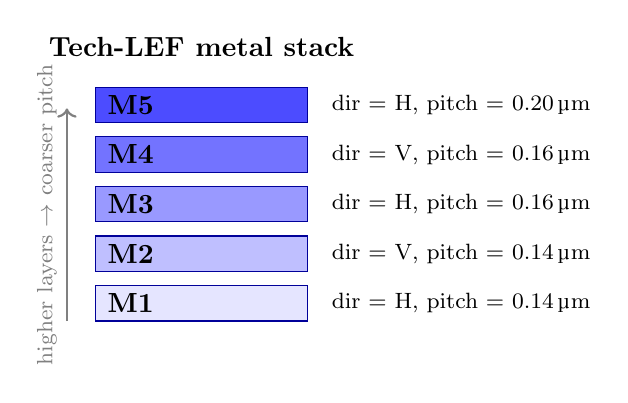
\begin{tikzpicture}[scale=0.9, every node/.style={font=\footnotesize}]
  % Layer stack
  \foreach \y/\name/\dir/\pitch in {0/M1/H/0.14, 1/M2/V/0.14, 2/M3/H/0.16, 3/M4/V/0.16, 4/M5/H/0.20} {
    \draw[fill=blue!\the\numexpr10+15*\y\relax, draw=blue!60!black] (0,\y*0.7) rectangle (3,\y*0.7+0.5);
    \node[black, font=\bfseries] at (0.5,\y*0.7+0.25) {\name};
    \node[anchor=west] at (3.2,\y*0.7+0.25) {dir = \dir, pitch = \pitch\,\si{\micro\meter}};
  }
  \node[anchor=south, font=\bfseries] at (1.5,3.6) {Tech-LEF metal stack};
  % Arrow indicating up
  \draw[->, thick, gray] (-0.4,0) -- (-0.4,3.0) node[midway, left, rotate=90, anchor=south] {higher layers $\to$ coarser pitch};
\end{tikzpicture}
\caption{A simplified tech-LEF view of the metal stack. Each \texttt{LAYER} declaration carries a \texttt{DIRECTION} (horizontal or vertical preferred routing) and a \texttt{PITCH}. The router uses these to lay tracks; the cell-LEF places its pin \texttt{RECT}s so they land on those tracks.}
\label{fig:metal-stack}
\end{figure}

\begin{pitfall}
\textbf{Four ways a LEF will silently wreck your block:}
\begin{itemize}[leftmargin=*,nosep]
  \item \textbf{Tech-LEF vs.\ cell-LEF confusion.} Loading two tech-LEFs (e.g., one from the foundry and one from the IP vendor) causes contradictory \texttt{LAYER} definitions. The tool may pick the wrong one without warning.
  \item \textbf{M1 pin access at advanced nodes.} At 7nm and below, M1 is so dense that a pin \texttt{RECT} may have zero legal access points after considering via rules. The router fails to connect it, even though DRC on the cell alone passes.
  \item \textbf{OBS misuse.} An overly aggressive \texttt{OBS} on M2 forces all routes to detour, blowing up congestion. Too little \texttt{OBS} and the router crosses an internal node, creating shorts at LVS.
  \item \textbf{Mismatched \texttt{SITE} definitions.} The std cell library was characterized on \texttt{SITE CoreSite} ($0.2 \times 1.2$), but the floorplan rows were generated on a slightly different site. Cells will not snap, and the tool emits thousands of placement-legality errors.
\end{itemize}
\end{pitfall}

\begin{sidebar}
\textbf{Tech-LEF vs.\ cell-LEF, and where LEF came from.} The \textbf{tech-LEF} is shipped by the foundry (or PDK provider) once per process node. It declares units, the metal stack (layer names, directions, pitches, min width, spacing), via definitions, and the placement \texttt{SITE} grid. The \textbf{cell-LEF} is shipped per standard cell library and contains one \texttt{MACRO} per cell. Both files are plain ASCII, historically defined by \textbf{Cadence} in the late 1980s as an open interchange format paired with \textbf{DEF} (Design Exchange Format) for post-placement data. The pair (LEF/DEF) is still the lingua franca that lets a Synopsys placer eat a TSMC library or a Cadence router eat a Samsung library without binary glue.
\end{sidebar}

\begin{pdnote}
\begin{itemize}[leftmargin=*,nosep]
  \item \textbf{Arm PD intern.} When a new tech drop lands, the first thing you do is diff the tech-LEF against the previous version: layer pitches, via rules, \texttt{SITE} sizes. A silent pitch change forces a full re-floorplan.
  \item \textbf{Generic PD engineer.} If a block has unroutable nets concentrated around one cell type, open that cell's LEF and inspect its M1 pin \texttt{RECT}s and \texttt{OBS} regions. Pin-access problems are visible at the library level long before they explode in the router log.
  \item \textbf{VLSI interview.} Expect the question: \emph{What is in a LEF file, and how is it different from a GDS?} The crisp answer is: LEF is the \textbf{abstract physical view} (bounding box, pins, blockages, on metal layers only) used by P\&R; GDS is the \textbf{full polygon-level layout} used only at LVS and tape-out.
\end{itemize}
\end{pdnote}

\begin{checkpoint}
You should now be able to: (1) state what LEF abstracts away and why, (2) name the two LEF flavors and what each contains, (3) read a \texttt{MACRO} block and identify \texttt{SIZE}, \texttt{SITE}, \texttt{PIN}, \texttt{PORT}, \texttt{LAYER}, \texttt{OBS}, (4) compute site occupancy for a given cell width.

\mnemonic{\textbf{``SIZE the cell, SITE the row, PIN the layer, OBS the rest.''} Four verbs map one-to-one onto the four LEF keywords the placer/router actually consults on every cell.}
\end{checkpoint}

\chapter[The Constraints File (SDC)]{The Constraints File (SDC): Telling the Tool What ``Working'' Means}

\begin{tldr}
\begin{itemize}
  \item \textbf{Last chapter:} LEF was the contract between the library and the placer, all physical and no time. \textbf{This chapter:} SDC is the contract between the designer and every timing-aware tool downstream, all time and no physics.
  \item \textbf{SDC} (Synopsys Design Constraints) is a \textbf{Tcl-based contract} that tells synthesis, STA, and PD what timing, power, and area the chip must hit.
  \item The \textbf{Big 5} commands are \texttt{create\_clock}, \texttt{set\_input\_delay}, \texttt{set\_output\_delay}, \texttt{set\_clock\_uncertainty}, and \texttt{set\_false\_path} / \texttt{set\_multicycle\_path}.
  \item \textbf{Setup} asks ``did data arrive \emph{before} the next capture edge minus the setup window?'' \textbf{Hold} asks ``did data wait \emph{long enough past} the current edge so the previous value was safely captured?''
  \item Slack is the headline number. Positive means met. Negative means the tool has work to do, or you have an SDC bug.
\end{itemize}
\end{tldr}

\section*{Opening: the contract nobody reads until it breaks}

A netlist by itself is silent about \textbf{when} signals should arrive. You can hand the same gate-level netlist to two engineers, give them two different SDC files, and they will ship two completely different chips. One will close at 1\,GHz; the other will look broken even though every transistor is identical. The constraints file is the difference.

This chapter pulls apart the SDC \textbf{piece by piece}. We will define clocks, anchor the boundary with input and output delays, do the slack arithmetic by hand for both setup and hold, and look at where engineers most often shoot themselves in the foot. By the end the file should stop feeling like a wall of Tcl and start feeling like a small, opinionated specification.

\section{What lives inside the SDC}

The SDC bundles three flavors of constraint into one file. \textbf{Timing} constraints define the clocks and the I/O delays that anchor every path. \textbf{Optimization} constraints (max transition, max capacitance, max fanout, input/output load) shape how the tool buffers and sizes the design. \textbf{Power} constraints cap dynamic and leakage budgets, often paired with a SAIF switching-activity file.

The lecturer is blunt about why SDC matters: it is read by \textbf{synthesis} (Design Compiler), by \textbf{STA} (PrimeTime), by \textbf{place-and-route} (ICC2 / Innovus), and by \textbf{formal} flows. Every downstream tool trusts it. If the SDC lies, every report based on it also lies.

\subsection{The timing waveform: launch, capture, slack}

\begin{figure}[h]
\centering
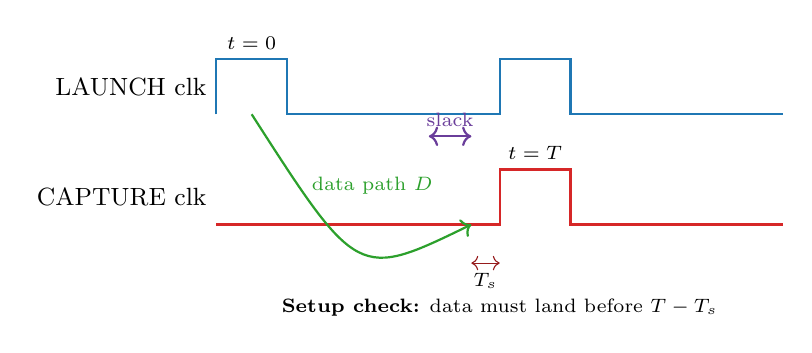
\begin{tikzpicture}[x=0.9cm, y=0.7cm]
  % Launch clock waveform
  \draw[thick, cKEY] (0,3) -- (0,4) -- (1,4) -- (1,3) -- (4,3) -- (4,4) -- (5,4) -- (5,3) -- (8,3);
  \node[left] at (0,3.5) {\small LAUNCH clk};
  \node[above] at (0.5,4) {\scriptsize $t=0$};

  % Capture clock waveform (one period later)
  \draw[thick, cPIT] (0,1) -- (4,1) -- (4,2) -- (5,2) -- (5,1) -- (8,1);
  \node[left] at (0,1.5) {\small CAPTURE clk};
  \node[above] at (4.5,2) {\scriptsize $t=T$};

  % Data arrival arrow
  \draw[->, thick, cCHECK] (0.5,3) .. controls (2,0) .. (3.6,1) ;
  \node[cCHECK] at (2.2,1.7) {\scriptsize data path $D$};

  % Setup window
  \draw[<->, cPIT!70!black] (3.6,0.3) -- (4,0.3);
  \node[below] at (3.8,0.3) {\scriptsize $T_s$};

  % Slack bracket
  \draw[<->, thick, cTLDR] (3.0,2.6) -- (3.6,2.6);
  \node[cTLDR, above] at (3.3,2.6) {\scriptsize slack};

  \node at (4,-0.5) {\scriptsize \textbf{Setup check:} data must land before $T - T_s$};
\end{tikzpicture}
\caption{Setup check on a single launch/capture pair. Slack $= T + \text{skew} - D - T_s$.}
\end{figure}

The launch flop fires its Q output at $t=0$. The signal walks through some combinational cloud, taking total delay $D$. The capture flop \textbf{samples} at $t=T$, but it needs the data to be stable for a small window $T_s$ \textbf{before} that edge. Anything left over is positive slack.

\begin{hook}
\textbf{``Launch lights the fuse; capture clips the wire.''} If the fuse burns too slowly (large $D$), capture's scissors slice through a signal still in motion. Setup violations are missed deadlines.
\end{hook}

\subsection{Anchoring the boundary: input and output delay}

\begin{figure}[h]
\centering
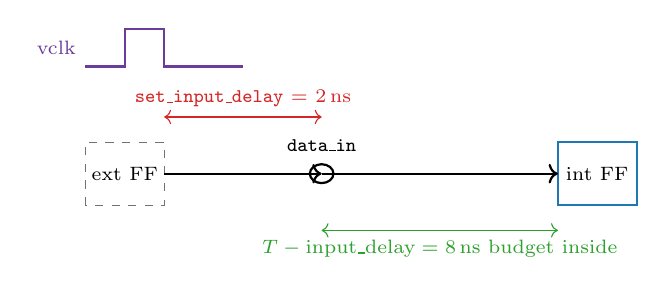
\begin{tikzpicture}[x=1cm, y=0.8cm]
  % Virtual external flop
  \draw[dashed, cGUT] (-3,1) rectangle (-2,2);
  \node at (-2.5,1.5) {\scriptsize ext FF};

  % Boundary port
  \draw[thick] (0,1.5) circle (0.15);
  \node[above] at (0,1.7) {\scriptsize \texttt{data\_in}};

  % Internal flop
  \draw[thick, cKEY] (3,1) rectangle (4,2);
  \node at (3.5,1.5) {\scriptsize int FF};

  % Arrows
  \draw[->, thick] (-2,1.5) -- (0,1.5);
  \draw[->, thick] (0,1.5) -- (3,1.5);

  % Brackets
  \draw[<->, cPIT] (-2,2.4) -- (0,2.4);
  \node[cPIT, above] at (-1,2.4) {\scriptsize \texttt{set\_input\_delay} = 2\,ns};

  \draw[<->, cCHECK] (0,0.6) -- (3,0.6);
  \node[cCHECK, below] at (1.5,0.6) {\scriptsize $T - \text{input\_delay} = 8$\,ns budget inside};

  % Virtual clock pulse
  \draw[thick, cTLDR] (-3,3.2) -- (-2.5,3.2) -- (-2.5,3.8) -- (-2,3.8) -- (-2,3.2) -- (-1,3.2);
  \node[cTLDR, left] at (-3,3.5) {\scriptsize vclk};
\end{tikzpicture}
\caption{\texttt{set\_input\_delay} models the time the signal already spent outside the block before reaching the port. The internal budget is what is left of the clock period.}
\end{figure}

\textbf{Input delay} says: ``by the time the signal walks in through this port, $X$\,ns of the clock period have already been consumed upstream.'' \textbf{Output delay} says: ``after the signal walks out through that port, the downstream flop still needs $Y$\,ns to capture it.'' Both are referenced to a clock, real or virtual, so STA knows what edge to measure against.

\begin{hook}
\textbf{``Input delay is rent paid before you moved in.''} The clock period is your apartment; the upstream logic already used some of the square footage. Whatever is left is yours to optimize.
\end{hook}

\section{The Big 5 SDC commands, by example}

\subsection{create\_clock and create\_generated\_clock}

\begin{lstlisting}[style=eda, language=tcl, caption={Defining a primary clock and a divide-by-2 generated clock.}]
# Primary 1 GHz clock on the CLK port
create_clock -name CLK_SYS -period 1.0 -waveform {0 0.5} \
    [get_ports CLK]

# Divide-by-2 generated clock on an internal flop's Q
create_generated_clock -name CLK_DIV2 -source [get_ports CLK] \
    -divide_by 2 [get_pins clkgen/div2_reg/Q]
\end{lstlisting}

A \textbf{primary clock} declares period and waveform at a port or pin. A \textbf{generated clock} is derived from a master with a known divide, multiply, or edge relationship. If you forget to declare a generated clock, STA will silently treat that internal node as just data and your reports will be wrong.

\subsection{set\_input\_delay, set\_output\_delay, virtual clocks}

\begin{lstlisting}[style=eda, language=tcl, caption={Boundary I/O timing referenced to a virtual clock.}]
# Virtual clock used only for I/O timing (no real pin)
create_clock -name VCLK -period 1.0

# Data arrives 0.3 ns after VCLK edge
set_input_delay  0.3 -clock VCLK [get_ports data_in*]

# Downstream FF needs 0.4 ns before its clock edge
set_output_delay 0.4 -clock VCLK [get_ports data_out*]
\end{lstlisting}

\textbf{Virtual clocks} exist purely as a timing reference; no pin in the block actually toggles with them. They are the standard trick when the real launching/capturing flop lives in another block and you only want to constrain the interface.

\subsection{set\_clock\_uncertainty, set\_false\_path, set\_multicycle\_path}

\begin{lstlisting}[style=eda, language=tcl, caption={Margin, exceptions, and multicycle relief.}]
# Account for jitter + a safety margin (pre-CTS uses larger value)
set_clock_uncertainty -setup 0.08 [get_clocks CLK_SYS]
set_clock_uncertainty -hold  0.03 [get_clocks CLK_SYS]

# Async config path: ignore for timing entirely
set_false_path -from [get_pins cfg_reg*/Q] -to [get_pins core/*/D]

# Two-cycle path: data is allowed 2T to settle, hold relative to launch
set_multicycle_path 2 -setup -from [get_pins slow_src/Q] -to [get_pins slow_dst/D]
set_multicycle_path 1 -hold  -from [get_pins slow_src/Q] -to [get_pins slow_dst/D]
\end{lstlisting}

\textbf{Uncertainty} folds jitter, skew estimate, and pessimism into one number that is subtracted from the available period. Pre-CTS the value is large because the clock tree does not exist yet; post-CTS it shrinks. \textbf{False paths} declare ``never time this.'' \textbf{Multicycle paths} say ``this path is allowed $N$ clock periods instead of one.''

\begin{gut}
The SDC has \texttt{create\_clock -period 2.0} on \texttt{CLK} and \texttt{set\_clock\_uncertainty -setup 0.15}. What is the effective period available for data-path delay before subtracting setup time and input/output delays?
\gutans{$T_{\text{eff}} = 2.0 - 0.15 = 1.85$\,ns. Uncertainty is consumed before any logic delay.}
\end{gut}

\begin{gut}
Why must a generated clock be \emph{declared} even though it is physically derived from a real flop driven by a real clock?
\gutans{Because STA needs to know the period and edge relationship so it can correctly time paths that launch on the master and capture on the generated clock (or vice versa). Without the declaration, STA treats the node as data, not as a clock, and reports nonsense.}
\end{gut}

\begin{pausebox}
So far: SDC = Tcl contract. The Big 5 are clock, input delay, output delay, uncertainty, and exceptions. Setup is ``arrive before deadline,'' hold is ``do not change too early.'' Next we do the math.
\end{pausebox}

\begin{keyidea}
The SDC is the \textbf{single source of truth} that converts a netlist into a timed promise: every downstream tool (synthesis, STA, PnR, signoff) measures success against the same clock periods, I/O delays, uncertainties, and exceptions you write here.
\end{keyidea}

\section{Worked example: setup slack arithmetic}

A single capture-to-launch pair with: launch edge at $t=0$, period $T=1.0$\,ns, combinational delay $D=0.8$\,ns, capture clock skew $\text{skew}=+0.05$\,ns (capture clock arrives \emph{later} than launch clock, helping setup), and capture flop setup window $T_s=0.10$\,ns.

\move{1} Write the setup-slack formula with numbers \emph{first}.
\[
\text{slack}_{\text{setup}} = T + \text{skew} - D - T_s = 1.0 + 0.05 - 0.8 - 0.10
\]

\move{2} Add the helpers, subtract the burdens.
\[
\text{slack}_{\text{setup}} = 1.05 - 0.90 = 0.15~\text{ns}
\]

\move{3} Positive. Setup is \textbf{met} with 150\,ps of margin.

\move{4} Generalize. The setup check at any endpoint is
\[
\boxed{\text{slack}_{\text{setup}} = (T_{\text{capture}} - T_{\text{launch}}) + \text{skew} - D_{\text{data}} - T_s - U}
\]
where $U$ is clock uncertainty.

Now hold. Same path, but hold time $T_h = 0.05$\,ns, and assume minimum data delay $D_{\min} = 0.20$\,ns from the same launch edge.

\move{5} Hold check arithmetic:
\[
\text{slack}_{\text{hold}} = D_{\min} - \text{skew} - T_h = 0.20 - 0.05 - 0.05 = 0.10~\text{ns}
\]
Positive. Hold is also met. Note that the same skew that \emph{helped} setup \emph{hurts} hold. This is why fixing one violation often breaks the other.

\move{6} Generalize:
\[
\boxed{\text{slack}_{\text{hold}} = D_{\min} - \text{skew} - T_h - U_{\text{hold}}}
\]

\move{7} Sanity. If skew were $+0.25$\,ns instead, hold slack would be $0.20 - 0.25 - 0.05 = -0.10$\,ns: a hold violation, even though setup got easier. Skew has opposite signs in the two equations. Memorize that.

\begin{pitfall}
The four most common SDC mistakes that get interns roasted in review:
\begin{itemize}
  \item \textbf{Missing generated clocks.} The divider's Q is treated as data, and downstream paths look magically clean (they are not).
  \item \textbf{No input/output delay on boundary ports.} STA assumes 0\,ns, so the inside-the-block budget looks like a full period. Real silicon then fails.
  \item \textbf{Wrong reference clock on \texttt{set\_input\_delay}.} You constrain against \texttt{CLK\_A} but the upstream block actually launches on \texttt{CLK\_B}. Slack numbers are fiction.
  \item \textbf{Using \texttt{set\_false\_path} as a hammer.} Engineers slap false paths on violating endpoints to make the report green. The path is still real silicon. The chip still fails. Use false paths only for genuinely asynchronous or unrelated logic.
\end{itemize}
\end{pitfall}

\begin{sidebar}[Sidebar: MMMC, modes, and corners]
Real chips do not live in one SDC. \textbf{MMMC} (Multi-Mode Multi-Corner) means the design is closed across a matrix of \textbf{modes} (functional, scan-shift, scan-capture, test, low-power) and \textbf{corners} (slow-slow / fast-fast process, high/low voltage, hot/cold). Each mode often has its own SDC because scan-shift typically uses a much slower clock and a different topology than functional mode. Signoff means every \texttt{(mode, corner)} pair closes timing simultaneously. This is where SDC discipline pays for itself, because a forgotten \texttt{set\_case\_analysis} on the scan-enable can silently disable timing across half the design.
\end{sidebar}

\begin{pdnote}
\begin{itemize}
  \item \textbf{Arm PD intern:} you will read SDC files on day one and write SDC tweaks by week two. Reviewers will ask you to justify every false path you add. Bring evidence, not vibes.
  \item \textbf{Generic foundry PD engineer:} MMMC closure is your full-time job. You spend more hours in PrimeTime reading SDC-driven reports than you do in the layout viewer. Tool-agnostic SDC fluency travels across Synopsys, Cadence, and Siemens flows.
  \item \textbf{VLSI interview:} this is \textbf{the} most asked topic in PD and STA interviews. Expect ``write the setup and hold slack equations,'' ``what is a virtual clock,'' ``when do you use multicycle vs false path,'' and ``draw the launch/capture waveform.'' If you can produce the equations and the diagram from this chapter on a whiteboard cold, you are ahead of 80\% of new grads.
\end{itemize}
\end{pdnote}

\begin{checkpoint}
You can now (a) name the Big 5 SDC commands and what each one anchors, (b) write the setup and hold slack equations and substitute numbers without looking them up, (c) explain why skew helps setup but hurts hold, and (d) spot the four common SDC mistakes in a code review. \mnemonic{Clock, in, out, jitter, exception. Setup arrives early; hold stays late.}
\end{checkpoint}

\chapter{The Technology File: Where Physics Becomes Rules}

\begin{tldr}
\begin{itemize}
  \item \textbf{Last chapter:} the SDC turned a netlist into a timed promise every tool measures against. \textbf{This chapter:} the tech file is the foundry rulebook every routed shape must obey before that promise can be cashed in silicon.
  \item The \textbf{technology file} is the foundry contract that turns silicon physics into machine-readable design rules your PD tool obeys layer by layer.
  \item It carries \textbf{layer definitions, min width/spacing, min area, via geometries, sheet resistance, thickness, permittivity, and colors} for multi-patterning.
  \item Without it, the router has \textbf{no legal moves}: every wire it draws would be a DRC violation waiting to happen.
  \item Two cousins exist in real flows: the older Cadence \texttt{.tf} format and the modern \textbf{tech-LEF} abstraction, often paired with an \texttt{ITF} for parasitic extraction.
\end{itemize}
\end{tldr}

\begin{hook}
Imagine handing a contractor a blueprint with no building code, no minimum stud spacing, no fire rating, no permitted materials. He builds whatever he wants and the inspector burns it down. That is exactly what a place-and-route tool would do without a tech file, except the inspector is the foundry mask shop and \enquote{burning it down} means a \$3M tapeout that yields zero working die. So how does a four-kilobyte ASCII file save a multi-million-dollar wafer run?
\end{hook}

\section{The Stack You Are Actually Routing On}

A modern CMOS chip is a sandwich of conducting metal layers separated by dielectric, stitched together by tiny vertical plugs called vias. The tech file describes \textbf{every one of those layers}, bottom to top, with the numbers a router needs to keep wires legal and signals fast. Layers near the substrate are \textbf{thin and tight} (good for short local nets, bad for current); layers up top are \textbf{thick and wide} (good for power and clock, bad for density).

\begin{figure}[h]
\centering
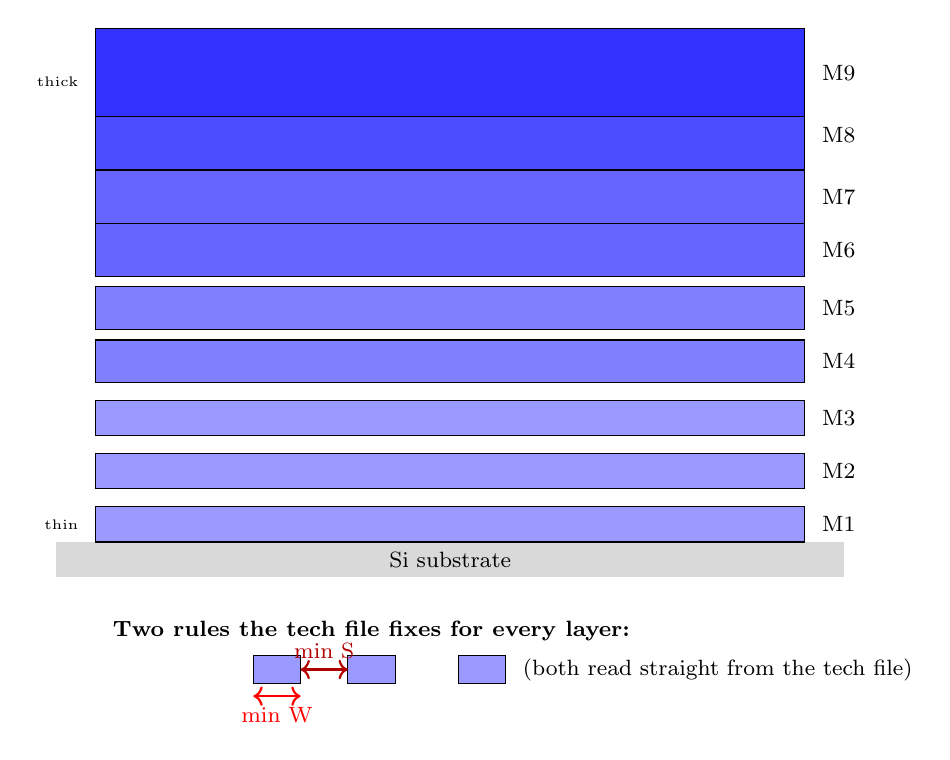
\begin{tikzpicture}[x=1cm,y=0.45cm]
  % substrate
  \fill[gray!30] (0,0) rectangle (10,1); \node at (5,0.5) {\footnotesize Si substrate};
  % metal stack alternating dielectric (light) and metal (dark)
  \foreach \i/\name/\h/\col in {
    1/M1/1.0/blue!40,
    2/M2/1.0/blue!40,
    3/M3/1.0/blue!40,
    4/M4/1.2/blue!50,
    5/M5/1.2/blue!50,
    6/M6/1.5/blue!60,
    7/M7/1.5/blue!60,
    8/M8/2.0/blue!70,
    9/M9/2.5/blue!80
  }{
    \pgfmathsetmacro{\ybot}{1 + (\i-1)*1.5}
    \fill[\col] (0.5,\ybot) rectangle (9.5,\ybot+\h);
    \draw (0.5,\ybot) rectangle (9.5,\ybot+\h);
    \node[right] at (9.6,\ybot+\h/2) {\footnotesize \name};
  }
  % min width / min spacing callout: drawn as a separate inset below the stack
  \begin{scope}[shift={(2.5,-3.0)}]
    \node[font=\footnotesize\bfseries] at (1.5,1.5) {Two rules the tech file fixes for every layer:};
    \fill[blue!40] (0.0,0) rectangle (0.6,0.8); \draw (0.0,0) rectangle (0.6,0.8);
    \fill[blue!40] (1.2,0) rectangle (1.8,0.8); \draw (1.2,0) rectangle (1.8,0.8);
    \draw[<->,thick,red] (0.0,-0.35) -- (0.6,-0.35);
    \node[below,font=\footnotesize\color{red}] at (0.3,-0.38) {min W};
    \draw[<->,thick,red!70!black] (0.6,0.4) -- (1.2,0.4);
    \node[above,font=\footnotesize\color{red!70!black}] at (0.9,0.45) {min S};
    \fill[blue!40] (2.6,0) rectangle (3.2,0.8); \draw (2.6,0) rectangle (3.2,0.8);
    \node[right,font=\footnotesize] at (3.3,0.4) {(both read straight from the tech file)};
  \end{scope}
  \node[left] at (0.4,1.5) {\tiny thin};
  \node[left] at (0.4,14) {\tiny thick};
\end{tikzpicture}
\caption{Metal stack M1 through M9. Lower layers are thin and dense; upper layers grow thicker for current handling. The red arrows on M2 show the two rules the tech file enforces everywhere: minimum width and minimum spacing.}
\end{figure}

\begin{keyidea}
The technology file is the \textbf{foundry-supplied rulebook} that names every physical layer, fixes its geometric and electrical parameters, and tells the PD tool exactly what shapes it is allowed to draw.
\end{keyidea}

\section{What Lives Inside the File}

Open a real tech file and you will see a layered structure: chip-level parameters first (chip X/Y, frequency, FFT area for RF flows), then a substrate and dielectric block, then a long tail of \textbf{metal and via blocks}. Each metal entry carries a layer number, a name, a color, sheet resistance, thickness, and the design rules that come with it. The dielectric entries carry \textbf{permittivity} (relative, unitless) and \textbf{thickness} in microns, because that is what an extractor needs to back out capacitance.

\begin{figure}[h]
\centering
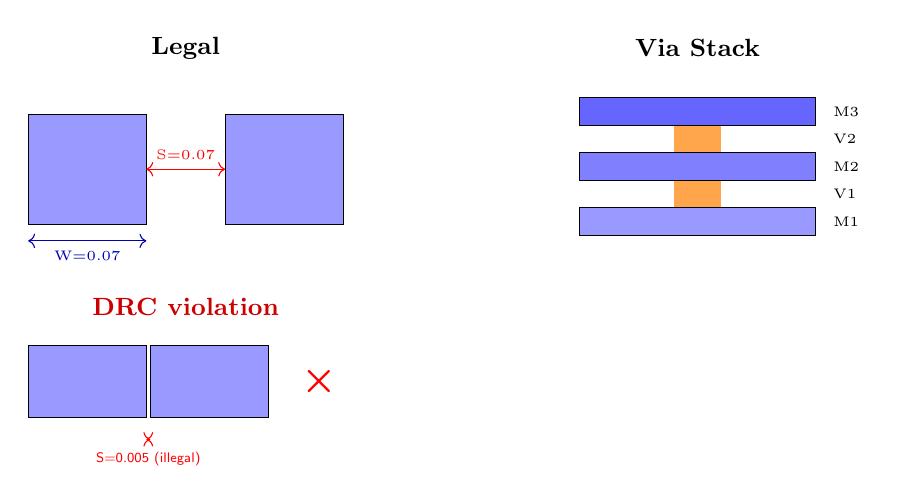
\begin{tikzpicture}[x=1cm,y=0.7cm]
  % LEFT: good spacing
  \node[font=\small\bfseries] at (2.5,5.2) {Legal};
  \fill[blue!40] (0.5,2) rectangle (2.0,4);
  \fill[blue!40] (3.0,2) rectangle (4.5,4);
  \draw (0.5,2) rectangle (2.0,4);
  \draw (3.0,2) rectangle (4.5,4);
  \draw[<->,red] (2.0,3) -- (3.0,3) node[midway,above,font=\tiny\color{red}]{S=0.07};
  \draw[<->,blue!70!black] (0.5,1.7) -- (2.0,1.7) node[midway,below,font=\tiny]{W=0.07};
  % via stack overlay on right column
  \node[font=\small\bfseries] at (9,5.2) {Via Stack};
  \fill[blue!40] (7.5,1.8) rectangle (10.5,2.3); \node[right,font=\tiny] at (10.6,2.05){M1};
  \fill[orange!70] (8.7,2.3) rectangle (9.3,2.8); \node[right,font=\tiny] at (10.6,2.55){V1};
  \fill[blue!50] (7.5,2.8) rectangle (10.5,3.3); \node[right,font=\tiny] at (10.6,3.05){M2};
  \fill[orange!70] (8.7,3.3) rectangle (9.3,3.8); \node[right,font=\tiny] at (10.6,3.55){V2};
  \fill[blue!60] (7.5,3.8) rectangle (10.5,4.3); \node[right,font=\tiny] at (10.6,4.05){M3};
  \draw (7.5,1.8) rectangle (10.5,2.3);
  \draw (7.5,2.8) rectangle (10.5,3.3);
  \draw (7.5,3.8) rectangle (10.5,4.3);
  % DRC violation row
  \node[font=\small\bfseries\color{red!80!black}] at (2.5,0.5) {DRC violation};
  \fill[blue!40] (0.5,-1.5) rectangle (2.0,-0.2);
  \fill[blue!40] (2.05,-1.5) rectangle (3.55,-0.2);
  \draw (0.5,-1.5) rectangle (2.0,-0.2);
  \draw (2.05,-1.5) rectangle (3.55,-0.2);
  \draw[<->,red] (2.0,-1.9) -- (2.05,-1.9);
  \node[font=\tiny\color{red},below] at (2.025,-1.95) {\textsf{S=0.005 (illegal)}};
  \node[font=\Large\bfseries\color{red}] at (4.2,-0.85) {$\boldsymbol{\times}$};
\end{tikzpicture}
\caption{Left: two M2 wires with the legal minimum spacing the tech file declares. Right: a via stack M1$\to$V1$\to$M2$\to$V2$\to$M3 with the vias defined as small square cuts inside larger metal landing pads. Bottom: the same two wires drawn too close, which the DRC engine flags instantly because the spacing rule was read straight from the tech file.}
\end{figure}

\begin{lstlisting}[style=eda,caption={Skeleton of a tech file fragment (illustrative)}]
chip_x = 1200
chip_y = 1200
tech_file = "rf28_v1.tf"
frequency = 2.4e9
layer substrate { rho = 10  ; thickness = 280 }
layer ild1      { eps_r = 4.2 ; thickness = 0.4 }
layer metal0    { num=1 ; rs=0.12 ; t=0.13 ; color=red    ; minW=0.07 ; minS=0.07 }
layer metal1    { num=2 ; rs=0.10 ; t=0.15 ; color=green  ; minW=0.07 ; minS=0.07 }
via   v1        { from=metal0 ; to=metal1 ; cut=0.07x0.07 ; enc=0.005 }
\end{lstlisting}

\subsection*{Memory hooks}

\begin{pdnote}
\textbf{Hook 1.} The \textbf{foundry stapler} \textit{slams} the rulebook onto your desk; lose it and your router \textit{flies blind into a million-dollar wall}.

\textbf{Hook 2.} \textbf{Dielectric layers} \textit{whisper} their permittivity to the \textbf{extractor}; misread them and your \textit{timing report lies to your face}.
\end{pdnote}

\subsection*{Gut checks}

\begin{gut}
You delete the via definition for V3 from the tech file and rerun routing. What breaks first? \gutans{The router cannot legally connect M3 to M4, so any net needing that transition fails (open net or DRC) and the tool errors out before completing.}
\end{gut}

\begin{gut}
Why is M9 drawn three times thicker than M1 in the stack figure? \gutans{Upper metals carry power and global clock; thicker metal lowers sheet resistance and IR drop. Lower metals stay thin to keep pitch tight for dense local routing.}
\end{gut}

\begin{pausebox}
Stop. Before reading on, predict: if a tech file lists \textbf{only} M1 through M5 but your floorplan needs a top-level clock mesh, what happens when you try to route the mesh on M6? Say it out loud.
\end{pausebox}

\section{Worked Example: Counting Tracks Across a Channel}

\textbf{Setup.} M2 has \textbf{min width $W = 0.07\,\mu m$} and \textbf{min spacing $S = 0.07\,\mu m$}. A routing channel is \textbf{5.0 microns wide}. How many M2 tracks fit?

\move{1} Substitute the numbers into the pitch definition:
\[
\text{pitch} = W + S = 0.07 + 0.07 = 0.14\,\mu m.
\]

\move{2} Divide the available channel width by the pitch:
\[
N = \left\lfloor \frac{5.0}{0.14} \right\rfloor = \lfloor 35.71 \rfloor = 35 \text{ tracks}.
\]

\move{3} Sanity check by rebuilding the total occupied width:
\[
35 \times 0.14 = 4.90\,\mu m \le 5.0\,\mu m. \checkmark
\]

\move{4} The leftover $0.10\,\mu m$ is not enough for a 36th track (would need another $0.14\,\mu m$), so 35 is tight and correct.

\begin{keyidea}
\textbf{Routing capacity per layer} is set entirely by the tech file. Change \textbf{minW} or \textbf{minS} by ten nanometers and your channel either fits the design or fails routing congestion.
\end{keyidea}

\section{Watch Out}

\begin{pitfall}
\textbf{Tech file vs tech-LEF.} They are siblings, not twins. The Cadence \texttt{.tf} is the older, richer foundry-format file (often paired with an \texttt{ITF} for extraction). \textbf{tech-LEF} is the LEF/DEF-style abstraction modern Synopsys and tool-agnostic flows consume. Some tools accept either depending on the flow; do not assume one is a drop-in replacement for the other. Always match the tech format to what your PnR tool expects in its reference flow doc.
\end{pitfall}

\begin{pitfall}
\textbf{Colors are not just metal names.} At advanced nodes (sub-20nm), the \texttt{color} field is not cosmetic. It encodes \textbf{mask assignment for multi-patterning}. Two same-color shapes that are too close are a \textbf{coloring violation}, distinct from a normal spacing DRC. Treat color as a hard physical attribute, not a label.
\end{pitfall}

\begin{sidebar}{Why advanced nodes make this file explode}
At 7nm and below, a single metal layer is printed across \textbf{multiple masks} (LELE, SADP, SAQP). The tech file now has to declare \textbf{decomposition rules}, \textbf{coloring constraints}, \textbf{cut-mask geometries}, and per-color minimum spacings. A 28nm tech file might be a few thousand lines; a 5nm tech file plus its rule decks pushes into the hundreds of thousands. The discipline is the same, the size is not.
\end{sidebar}

\begin{pdnote}
\textbf{Why PD cares (three lenses):}
\begin{itemize}
  \item \textbf{Arm PD intern:} You will never write a tech file, but on day one you will load one and \texttt{grep} it for layer counts, min pitches, and via definitions to sanity check your floorplan.
  \item \textbf{Generic foundry PD engineer:} You consume the PDK as ground truth. When a router complains \enquote{no legal via found,} the answer is in the tech file's via section nine times out of ten.
  \item \textbf{VLSI interview:} \enquote{What is in a tech file and why do you need it?} is a layup question. Name layer defs, design rules, vias, RC parameters, and units. Bonus points for distinguishing \texttt{.tf} from tech-LEF.
\end{itemize}
\end{pdnote}

\begin{checkpoint}
\textbf{You should now be able to:}
\begin{itemize}
  \item Name at least five categories of information stored in a tech file.
  \item Compute routing pitch and tracks per channel from min width and min spacing.
  \item Explain the difference between \texttt{.tf} and tech-LEF in one sentence.
  \item Say why coloring fields stop being decorative at advanced nodes.
\end{itemize}

\mnemonic{\textbf{LIVR-C}: \textbf{L}ayers, \textbf{I}LD/permittivity, \textbf{V}ias, \textbf{R}ules (W/S/area), \textbf{C}olors. Five buckets, one file, every PD flow.}
\end{checkpoint}

\chapter{The DEF File: A Snapshot of Where Everything Lives}

\begin{tldr}
\begin{itemize}
  \item \textbf{Last chapter:} the tech file listed every legal shape on every layer. \textbf{This chapter:} the DEF records exactly which legal shapes ended up where, snapshot by snapshot through the flow.
  \item \textbf{DEF} (Design Exchange Format) is an ASCII file that captures the \textbf{current physical state} of the design: die shape, rows, instance placement, IO pin locations, and (later) full routing.
  \item DEF is emitted at \textbf{every major PD checkpoint} (post-floorplan, post-place, post-CTS, post-route); same file format, increasing completeness at each stage.
  \item \textbf{LEF + DEF together} give you enough to fully visualize a design in a layout viewer with no GDS in sight; GDS is for the fab, DEF is the working format used \emph{during} PD.
\end{itemize}
\end{tldr}

\begin{hook}
You have a netlist that says \emph{what} the design is and a LEF that says \emph{what each cell looks like}. Hand both to a tool and it still has no idea where to put anything. Somewhere there has to be a file that says \textbf{``this exact instance sits at (12.5, 7.5) microns, oriented north, and is fixed.''} That file gets rewritten after floorplan, after place, after CTS, after route. Same name. Same format. Different snapshot. What is inside it?
\end{hook}

\section{What DEF Actually Is}

\textbf{DEF} stands for \textbf{Design Exchange Format}. It is a plain-text file that describes the physical structure of a specific design instance: the die outline, the rows that standard cells slot into, the placement of every component, the IO pin locations on the boundary, and (after routing) the full wire and via geometry.

LEF tells the tool what a NAND2 cell physically looks like in the abstract. DEF tells the tool that instance \texttt{u\_alu/g\_carry} of that NAND2 sits at coordinate (12500, 7500) facing north. One is library, one is design.

\begin{keyidea}
A DEF file is a \textbf{textual snapshot of the design's physical state} at one point in the PD flow; LEF describes cells in the abstract, DEF describes \textbf{this design's instances} in concrete coordinates.
\end{keyidea}

\section{The Floorplan View}

The clearest mental picture of what DEF encodes is the floorplan itself. A die boundary, a core area inside it, IO pins around the edge, a few hard macros pre-placed, and standard cell rows filling the rest. Every one of those geometric facts has a DEF section behind it.

\begin{figure}[h]
\centering
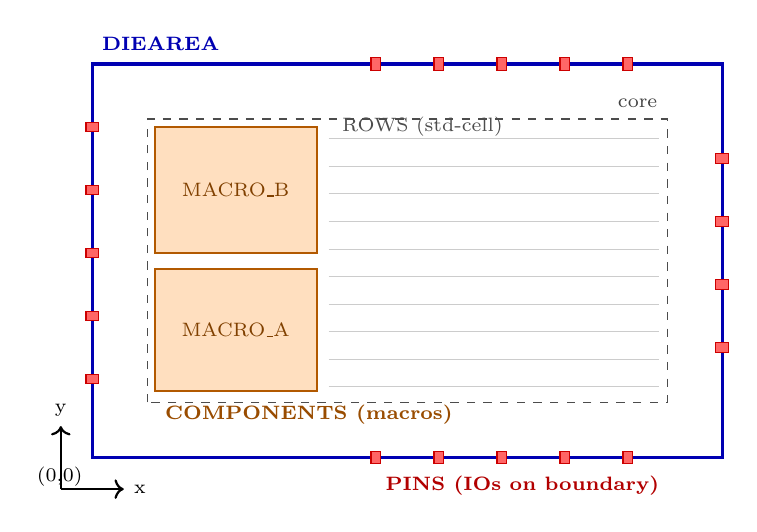
\begin{tikzpicture}[every node/.style={font=\scriptsize}]
  % DIEAREA
  \draw[very thick, blue!70!black] (0,0) rectangle (8,5);
  \node[blue!70!black, anchor=south west, font=\scriptsize\bfseries] at (0,5.05) {DIEAREA};

  % Core boundary
  \draw[dashed, gray!60!black] (0.7,0.7) rectangle (7.3,4.3);
  \node[gray!50!black, anchor=south east, font=\scriptsize] at (7.3,4.32) {core};

  % Standard cell rows
  \foreach \y in {0.9,1.25,1.6,1.95,2.3,2.65,3.0,3.35,3.7,4.05} {
    \draw[gray!40, line width=0.3pt] (3.0,\y) -- (7.2,\y);
  }
  \node[gray!60!black, anchor=west] at (3.05,4.2) {ROWS (std-cell)};

  % Macros
  \draw[fill=orange!25, draw=orange!70!black, thick] (0.8,0.85) rectangle (2.85,2.4);
  \node[orange!50!black] at (1.82,1.62) {MACRO\_A};
  \draw[fill=orange!25, draw=orange!70!black, thick] (0.8,2.6) rectangle (2.85,4.2);
  \node[orange!50!black] at (1.82,3.4) {MACRO\_B};
  \node[orange!60!black, anchor=west, font=\scriptsize\bfseries] at (0.8,0.55) {COMPONENTS (macros)};

  % IO pins around boundary
  \foreach \y in {1.0,1.8,2.6,3.4,4.2} {
    \draw[fill=red!60, draw=red!80!black] (-0.08,\y-0.06) rectangle (0.08,\y+0.06);
  }
  \foreach \y in {1.4,2.2,3.0,3.8} {
    \draw[fill=red!60, draw=red!80!black] (7.92,\y-0.06) rectangle (8.08,\y+0.06);
  }
  \foreach \x in {3.6,4.4,5.2,6.0,6.8} {
    \draw[fill=red!60, draw=red!80!black] (\x-0.06,-0.08) rectangle (\x+0.06,0.08);
    \draw[fill=red!60, draw=red!80!black] (\x-0.06,4.92) rectangle (\x+0.06,5.08);
  }
  \node[red!70!black, anchor=west, font=\scriptsize\bfseries] at (3.6,-0.35) {PINS (IOs on boundary)};

  % Origin marker
  \draw[->, thick] (-0.4,-0.4) -- (0.4,-0.4) node[right] {x};
  \draw[->, thick] (-0.4,-0.4) -- (-0.4,0.4) node[above] {y};
  \node[anchor=north east] at (0,0) {(0,0)};
\end{tikzpicture}
\caption{Floorplan-style picture of what a DEF file encodes. The die outline is the \textbf{DIEAREA} polygon, two pre-placed hard macros and the standard-cell rows live in \textbf{COMPONENTS} and \textbf{ROWS}, and the IO ports on the boundary are \textbf{PINS}. Each visible thing in this picture maps to one DEF section.}
\label{fig:def-floorplan}
\end{figure}

The DIEAREA polygon is walked \textbf{clockwise from the origin}, and order matters; reversing it flips the inside/outside semantics. The rows tile the inner core. The macros sit at fixed coordinates that the floorplanner has already committed to. The IO pads sit on the die edge.

\begin{hook}
Picture a \textbf{stage manager's set diagram} taped backstage: every prop (instance) has an X mark, every entrance (pin) is on the perimeter, every dancer's lane (row) is chalked across the floor. Lose the diagram mid-show and the next scene change collides two macros, which in silicon means DRC errors before you can spell ``re-floorplan.''
\end{hook}

\section{Inside the File}

Here is what the relevant sections look like in the actual ASCII. Names are illustrative; the keywords (\texttt{DIEAREA}, \texttt{ROW}, \texttt{COMPONENTS}, \texttt{PINS}, \texttt{NETS}) are not.

\begin{lstlisting}[style=eda,caption={Skeleton of a DEF file. Each major section ends with an explicit \texttt{END} keyword.},label={lst:def-skeleton}]
VERSION 5.8 ;
DIVIDERCHAR "/" ;
BUSBITCHARS "[]" ;
DESIGN top_block ;
UNITS DISTANCE MICRONS 1000 ;

DIEAREA ( 0 0 ) ( 0 38000 ) ( 14000 38000 )
        ( 14000 22000 ) ( 18000 22000 ) ( 18000 0 ) ;

ROW ROW_0 CORE 100 100 N DO 420 BY 1 STEP 200 1400 ;

COMPONENTS 4 ;
  - ENDCAP_L_0  TAPCELL_X1   + FIXED ( 100   100 ) N ;
  - u_alu/g_carry  NAND2_X1  + PLACED ( 12500 7500 ) N ;
  - u_alu/g_sum    XOR2_X2   + PLACED ( 13200 7500 ) FN ;
  - u_ctrl/fsm_q   DFFR_X1   + PLACED ( 4800  9100 ) S ;
END COMPONENTS

PINS 3 ;
  - clk + NET clk + DIRECTION INPUT + USE SIGNAL
        + LAYER M4 ( -70 0 ) ( 70 140 )
        + FIXED ( 9000 38000 ) N ;
  - rst_n + NET rst_n + DIRECTION INPUT + USE SIGNAL
        + LAYER M4 ( -70 0 ) ( 70 140 )
        + FIXED ( 11000 38000 ) N ;
  - q_out + NET q_out + DIRECTION OUTPUT + USE SIGNAL
        + LAYER M4 ( -70 0 ) ( 70 140 )
        + FIXED ( 18000 12000 ) E ;
END PINS

NETS 2 ;
  - n_carry ( u_alu/g_carry Z ) ( u_alu/g_sum A ) ;
  - clk     ( PIN clk ) ( u_ctrl/fsm_q CK ) ;
END NETS

END DESIGN
\end{lstlisting}

Note three things. First, every component line carries its \textbf{reference cell name} (so the tool can look the geometry up in LEF), its \textbf{placement status} (\texttt{FIXED} vs.\ \texttt{PLACED} vs.\ \texttt{UNPLACED}), and its \textbf{orientation} (\texttt{N}, \texttt{S}, \texttt{FN}, etc.). Second, the file lists a count after each section header (\texttt{COMPONENTS 4 ;}) so the parser can pre-allocate. Third, all coordinates are integers in DEF database units, not microns.

\begin{gut}
In Listing \ref{lst:def-skeleton}, which two instances are \textbf{fixed} and cannot be moved by the placer, and which can?
\gutans{\texttt{ENDCAP\_L\_0} is \texttt{FIXED} (physical-only end-cap cell, locked at floorplan time). The three logical instances (\texttt{u\_alu/g\_carry}, \texttt{u\_alu/g\_sum}, \texttt{u\_ctrl/fsm\_q}) are \texttt{PLACED}, meaning the placer chose locations but is allowed to refine them in subsequent stages unless promoted to \texttt{FIXED}.}
\end{gut}

\section{DEF Lives at Every PD Checkpoint}

This is the part most beginners miss. DEF is not a one-shot file. The \textbf{same format} is emitted by the tool after each major stage of the PD flow, with progressively more sections populated. The floorplan-stage DEF has rows and macros but empty \texttt{NETS} geometry. The post-route DEF has every wire segment and every via.

\begin{figure}[h]
\centering
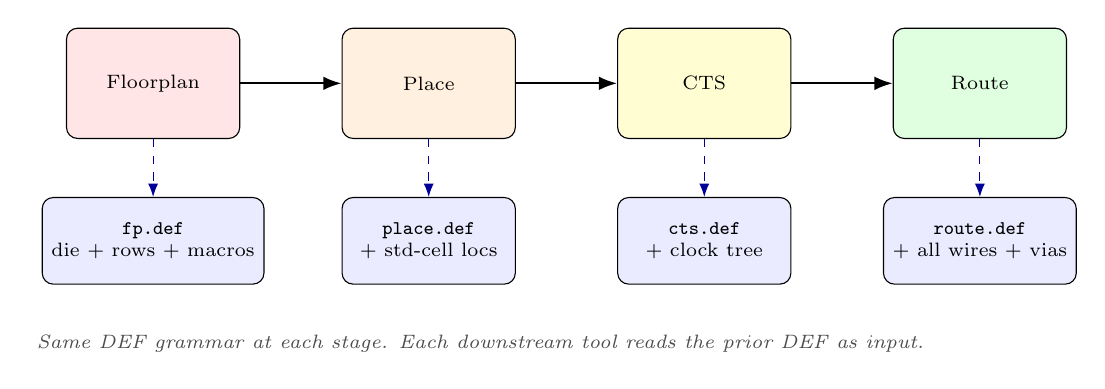
\begin{tikzpicture}[
  every node/.style={font=\scriptsize},
  stage/.style={draw, rounded corners, minimum width=22mm, minimum height=14mm, align=center},
  defbox/.style={draw, fill=blue!8, rounded corners, minimum width=22mm, minimum height=11mm, align=center, font=\scriptsize}
]
  \node[stage, fill=red!10]    (fp)  at (0,2)   {Floorplan};
  \node[stage, fill=orange!12] (pl)  at (3.5,2) {Place};
  \node[stage, fill=yellow!18] (cts) at (7.0,2) {CTS};
  \node[stage, fill=green!12]  (rt)  at (10.5,2){Route};

  \draw[-Latex, thick] (fp) -- (pl);
  \draw[-Latex, thick] (pl) -- (cts);
  \draw[-Latex, thick] (cts) -- (rt);

  \node[defbox] (d1) at (0,0)   {\texttt{fp.def}\\die + rows + macros};
  \node[defbox] (d2) at (3.5,0) {\texttt{place.def}\\+ std-cell locs};
  \node[defbox] (d3) at (7.0,0) {\texttt{cts.def}\\+ clock tree};
  \node[defbox] (d4) at (10.5,0){\texttt{route.def}\\+ all wires + vias};

  \draw[-Latex, dashed, blue!60!black] (fp) -- (d1);
  \draw[-Latex, dashed, blue!60!black] (pl) -- (d2);
  \draw[-Latex, dashed, blue!60!black] (cts) -- (d3);
  \draw[-Latex, dashed, blue!60!black] (rt) -- (d4);

  \node[anchor=west, font=\scriptsize\itshape, gray!60!black] at (-1.6,-1.3)
    {Same DEF grammar at each stage. Each downstream tool reads the prior DEF as input.};
\end{tikzpicture}
\caption{DEF is both an \textbf{output} of every PD stage and the \textbf{input} to the next. The grammar never changes; only the populated sections grow. \texttt{NETS} routing geometry is empty until after detailed routing.}
\label{fig:def-stages}
\end{figure}

This is why ``DEF file'' on its own is ambiguous in conversation. A senior PD engineer will ask \emph{which} DEF: the post-place one or the post-route one. They are very different in size and in what they let you do.

\begin{hook}
Think of DEF like the \textbf{photo a contractor texts you each Friday}. Week 1 is just the foundation slab (floorplan). Week 5 is framing (placement). Week 9 has wiring (route). Same camera, same angle, more stuff in every shot. Skip a week's photo and the next subcontractor shows up to a job site they cannot read.
\end{hook}

\begin{pausebox}
Pause. You inherit a directory with three DEFs named \texttt{a.def}, \texttt{b.def}, and \texttt{c.def} and no documentation. Which one diff would tell you which file came from which stage \textbf{without opening a layout viewer}? What grep would you reach for first?
\end{pausebox}

\section{Worked Example: Coordinate Arithmetic}

DEF coordinates are integers, not microns. The conversion factor lives in the \texttt{UNITS} statement at the top of the file.

\textbf{Problem.} The DEF in Listing \ref{lst:def-skeleton} starts with \texttt{UNITS DISTANCE MICRONS 1000}. An instance is written as \texttt{PLACED ( 12500 7500 ) N}. What is its physical placement in microns, and what is the smallest distance the format can represent?

\move{1} \textbf{Read the scale.} \texttt{UNITS DISTANCE MICRONS 1000} means \textbf{1 micron equals 1000 DEF database units}. So 1 DEF unit equals \(1\,\mu\text{m}/1000 = 1\,\text{nm}\).

\move{2} \textbf{Convert the X coordinate.} \(12500\) DEF units \(\times\, \tfrac{1\,\mu\text{m}}{1000\,\text{units}} = 12.5\,\mu\text{m}\).

\move{3} \textbf{Convert the Y coordinate.} \(7500 / 1000 = 7.5\,\mu\text{m}\).

\move{4} \textbf{Resolution.} The smallest non-zero distance representable is \textbf{1 nm}, since coordinates must be integers in DEF units.

\move{5} \textbf{What changes at a finer node.} For a 7\,nm flow you often see \texttt{UNITS DISTANCE MICRONS 2000}, meaning 1 DEF unit \(= 0.5\,\text{nm}\). The same coordinate string \texttt{12500} now means \(12500/2000 = 6.25\,\mu\text{m}\), which is why you \textbf{cannot copy coordinates between DEFs with different UNITS scales} without rescaling.

\begin{gut}
A DEF declares \texttt{UNITS DISTANCE MICRONS 2000} and pins one IO at \texttt{( 36000 18000 )}. Where does that pin physically sit?
\gutans{\(36000/2000 = 18\,\mu\text{m}\) in X and \(18000/2000 = 9\,\mu\text{m}\) in Y. Note that if you had assumed the previous file's 1000 scale, you would have placed it at (36, 18) and been off by 2$\times$ in both axes, which is a classic ECO bug.}
\end{gut}

\begin{pitfall}
\textbf{DEF traps that bite new PD engineers.}
\begin{itemize}
  \item \textbf{DEF vs.\ LEF confusion.} LEF is the \emph{library} physical view (what a cell looks like, reusable across designs). DEF is the \emph{design} snapshot (where every instance of every cell sits in \emph{this} chip). LEF is mandatory to start PD; DEF is not, because the floorplan tool can generate the first DEF itself.
  \item \textbf{Coordinate-unit mismatch.} Forgetting to read \texttt{UNITS DISTANCE MICRONS} before doing arithmetic on DEF coordinates is the single most common rookie error. Always grep the header first.
  \item \textbf{DEF is both output and input.} The same file role flips at every stage boundary. Post-route DEF is an output of detailed routing \textbf{and} the input to signoff extraction, formal LVS, and any later ECO. Treating it as one or the other (but not both) leads to broken handoff scripts.
  \item \textbf{DEF is not GDS.} Tape-out goes out as \textbf{GDSII} (binary, polygon-level mask data). DEF stays inside the PD environment. You never hand DEF to the foundry as final artwork.
\end{itemize}
\end{pitfall}

\begin{sidebar}
\textbf{DEF as a design-exchange artifact.} The name is not a coincidence. DEF was invented so that two teams (or two companies) could hand a partial physical implementation back and forth without sharing the whole tool database. A vendor can deliver a hardened block as \textbf{LEF + post-route DEF}; the customer imports it into their top-level integration without ever seeing the source RTL or the cell internals.

\textbf{DEF in ECO flows.} Engineering Change Orders work the same way. The signoff team writes a tiny \textbf{ECO patch DEF} that touches only the instances and nets that changed, and the implementation tool reads it as an incremental input over the existing routed DEF. Same format, smaller delta, much faster iteration than redoing place-and-route from scratch.
\end{sidebar}

\begin{pdnote}
\textbf{Why PD cares.}
\begin{itemize}
  \item \textbf{ARM PD intern lens:} on your first day, you will be asked to load \texttt{*.def} into Innovus or ICC2 and screenshot the floorplan; knowing which DEF (floorplan vs.\ post-route) you are looking at is half of not embarrassing yourself in the standup.
  \item \textbf{Generic foundry-flow PD engineer lens:} every stage script writes a DEF and the next stage reads it; broken handoffs almost always trace to a \texttt{UNITS} mismatch, a missing \texttt{PINS} section, or a stale post-place DEF being fed into routing instead of the post-CTS version.
  \item \textbf{VLSI interview lens:} expect ``what is the difference between LEF and DEF?'' and ``at what stages is a DEF file generated?''; the right answers are \emph{library vs.\ design instance} and \emph{after floorplan, place, CTS, and route}.
\end{itemize}
\end{pdnote}

\begin{checkpoint}
You should now be able to: (1) state that DEF is an ASCII snapshot of the design's physical state and name its main sections (\texttt{DIEAREA}, \texttt{ROW}, \texttt{COMPONENTS}, \texttt{PINS}, \texttt{NETS}), (2) explain why DEF is emitted at every PD checkpoint and how the same format grows in completeness across stages, (3) convert DEF database units to microns using the \texttt{UNITS DISTANCE MICRONS} scale, and (4) cleanly separate LEF (library, abstract cell view) from DEF (this design's instance placement) and from GDS (final mask artwork for the fab).

\mnemonic{DRCPN: \textbf{D}IEAREA, \textbf{R}OW, \textbf{C}OMPONENTS, \textbf{P}INS, \textbf{N}ETS}
\end{checkpoint}

\chapter{The CTS Spec: How You Tell the Tool to Build the Clock}

\begin{tldr}
\begin{itemize}
  \item \textbf{Last chapter:} DEF was the snapshot of where everything lives. \textbf{This chapter:} the CTS spec is the instructions for how the biggest single set of those things (the clock network) gets built between post-place and post-route DEF.
  \item The \textbf{CCOPT spec} is a Tcl/CSV artifact that tells Innovus the per-clock targets: \textbf{skew, latency, max transition, NDR, skew groups, useful-skew limits}, and mesh boundaries.
  \item Clock nets do not route like data nets. They get \textbf{non-default routing rules (NDR)} for shielding and width, and they get \textbf{balanced} across endpoints inside a skew group.
  \item Get the spec wrong and you spend a week chasing a clock spine that ate three M5 tracks too many or a generated clock that drifted 60~ps from its master.
\end{itemize}
\end{tldr}

\begin{hook}
Open post-place DEF and post-route DEF side by side. Same netlist, you would think, with wires filled in. Except the cell count grew by roughly five percent, every flop has a new buffer chain feeding it, and the clock nets look nothing like what synthesis handed you. Something ran in between that cloned hundreds of buffers, picked routing layers the data nets are not allowed to touch, and balanced arrival times to within ten picoseconds at thousands of sinks. What did that thing read to know what to do?
\end{hook}

\section{What the CTS Spec Actually Is}

The \textbf{CTS spec} (in Innovus, the \textbf{CCOPT spec}) is a small text file (Tcl directives plus an optional CSV) that tells \texttt{ccopt\_design} how to build and balance the clock network. It is not RTL, it is not constraints in the SDC sense, and it is not floorplan. It is a \textbf{per-clock recipe}: for each clock root, what is the target latency, what is the target skew, which other clocks share its skew budget, what routing rule do the segments use, and where (if anywhere) does the network transition from a tree to a mesh.

The Synopsys ICC2 equivalent lives inside \texttt{clock\_opt} and a \texttt{.ccopt}-equivalent CSV; the vocabulary is nearly identical, the keywords differ.

\begin{keyidea}
The CTS spec is the \textbf{only place in the flow where you express clock-network intent declaratively}; everything else (placement, route, sign-off) just reacts to the tree CCOPT builds from it.
\end{keyidea}

A realistic CCOPT spec snippet looks like this:

\begin{lstlisting}[style=eda, caption={Excerpt from a CCOPT spec for a two-clock subsystem.}, label={lst:ccopt-spec}]
# ---- global CTS knobs ----
set_ccopt_property buffer_cells       {CKBUFM8 CKBUFM12 CKBUFM16}
set_ccopt_property inverter_cells     {CKINVM8 CKINVM12 CKINVM16}
set_ccopt_property clock_gating_cells {CKLNQM8 CKLNQM12}
set_ccopt_property target_max_trans   80ps
set_ccopt_property use_inverters      true

# ---- per-clock targets ----
create_ccopt_clock_tree clk_core -source [get_db pins CLKGEN/clk_core]
set_ccopt_property -clock_tree clk_core target_skew    50ps
set_ccopt_property -clock_tree clk_core target_latency 350ps
set_ccopt_property -clock_tree clk_core routing_rule   NDR_2W2S_M5M6

create_ccopt_clock_tree clk_io   -source [get_db pins CLKGEN/clk_io]
set_ccopt_property -clock_tree clk_io   target_skew    75ps
set_ccopt_property -clock_tree clk_io   routing_rule   NDR_1W2S_M4M5

# ---- skew groups ----
create_ccopt_skew_group -name core_grp \
    -sources {CLKGEN/clk_core CLKGEN/clk_core_div2}
create_ccopt_skew_group -name io_grp   -sources {CLKGEN/clk_io}
create_ccopt_skew_group -name dft_grp  -sources {CLKGEN/clk_dft}

# ---- run it ----
ccopt_design -cts
\end{lstlisting}

Four things are happening here. The first block sets the \textbf{cell palette} CCOPT is allowed to clone from. The second creates a tree per clock root with its own skew and latency targets. The third declares \textbf{which clocks share a balance budget}. The fourth runs the engine.

\begin{hook}
A CCOPT spec is the \textbf{conductor's score} for the orchestra of flops. Skip the part that says ``violins and violas share a downbeat'' and the section drifts a quarter note; in silicon a quarter note is 60~ps of skew and your launch-capture pair misses by an entire setup margin.
\end{hook}

\section{Clock Skew Groups}

\textbf{Skew} is the difference in clock arrival time between two endpoints. CCOPT will spend buffers and routing to flatten skew, but only \emph{within a skew group}. Two clocks in different groups are allowed to drift relative to each other because the tool assumes you do not have any path that closes timing between them.

You put clocks in the same skew group when \textbf{paths exist between their endpoints} (synchronous CDC, generated clocks of a common master, mux-selected clocks that converge on the same flops). You keep them in separate groups when the domains are \textbf{truly asynchronous} (handled by a CDC synchronizer) so CCOPT does not waste buffers trying to flatten a difference no timing path cares about.

\begin{gut}
You have \texttt{clk\_core} at 800~MHz and \texttt{clk\_core\_div2} at 400~MHz, generated from \texttt{clk\_core} by a divide-by-two flop. A handful of paths cross from div2 flops back to core flops. Same group or different?
\gutans{Same group. The two clocks share endpoints, and you need their insertion delays balanced so the cross-domain paths close at sign-off. If you leave the divider in its own group, CCOPT balances the div2 tree to itself and the divider output drifts ~40--80~ps from the core tree, blowing the cross-domain setup checks even though the RTL is perfectly synchronous.}
\end{gut}

\subsection*{Worked numbers: three clocks, two groups}

Take three clocks on a small subsystem:

\begin{center}
\begin{tabular}{lll}
\textbf{Clock} & \textbf{Frequency} & \textbf{Endpoints} \\
\hline
\texttt{clk\_core}      & 800~MHz & CPU pipeline flops \\
\texttt{clk\_core\_div2} & 400~MHz & Cache tag array (same CPU) \\
\texttt{clk\_io}        & 400~MHz & PHY-facing flops (async to core) \\
\texttt{clk\_dft}       & 100~MHz & Scan chain only \\
\end{tabular}
\end{center}

Group \texttt{clk\_core} and \texttt{clk\_core\_div2} together because cache-tag-to-pipeline paths exist. Leave \texttt{clk\_io} on its own (CDC synchronizer at the boundary). Leave \texttt{clk\_dft} on its own (only active in scan mode, never racing functional paths).

Slack benefit of grouping the two core clocks: if each tree is built independently CCOPT meets a 50~ps intra-tree skew target but \textbf{intra-tree alignment between the two trees drifts by typically 60--100~ps}. Group them and that drift collapses into the same 50~ps target, recovering roughly 60~ps of slack on every cross-clock path. On an 800~MHz clock (1.25~ns period) that is almost five percent of the budget handed back for free.

\begin{pausebox}
Stop here. Write down the rule of thumb in your own words: \emph{when do two clocks belong in the same skew group?} If the answer in your head is anything other than ``when timing paths exist between their endpoints,'' re-read the last two paragraphs before continuing. The rest of this chapter assumes you have this reflex.
\end{pausebox}

\section{NDR: Non-Default Routing Rules}

Clock nets are skew-sensitive, which means they are crosstalk-sensitive, which means they get \textbf{routed differently from data nets}. A \textbf{Non-Default Routing rule (NDR)} bumps wire width, wire spacing, or both, and optionally adds \textbf{shield wires} tied to power or ground on either side.

The shorthand \textbf{2W2S} means double width and double spacing relative to the default for that layer. \textbf{1W2S} means default width, double spacing. Width fights resistance and reduces RC delay variation; spacing fights coupling capacitance to neighbors and reduces aggressor-induced skew.

\subsection*{Worked numbers: 2W2S on M5}

Assume M5 has \textbf{default width 0.07~$\mu$m and default spacing 0.07~$\mu$m}, so default pitch (center to center of adjacent tracks) is $0.07 + 0.07 = 0.14~\mu$m.

\move{1} A 2W2S NDR sets effective width to $2 \times 0.07 = 0.14~\mu$m and effective spacing to $2 \times 0.07 = 0.14~\mu$m. Pitch between two NDR clock wires becomes $0.14 + 0.14 = 0.28~\mu$m. \textbf{Each NDR clock wire consumes the area of two default tracks plus the gap}, so the effective track footprint is $0.28~\mu$m versus $0.14~\mu$m for a data net. One clock route eats \textbf{two default M5 tracks}.

\move{2} If the spec demands shielding (one VSS wire on each side at default spacing), tack on another $2 \times 0.14~\mu$m. Total footprint per shielded clock wire: $0.28 + 0.28 = 0.56~\mu$m, or \textbf{four default M5 tracks per clock net}.

\move{3} A clock spine of 8 parallel routes therefore consumes $8 \times 4 = 32$~M5 tracks. On a 100~$\mu$m wide channel with M5 pitch 0.14~$\mu$m, the channel has roughly 714 tracks total, so the spine eats \textbf{about 4.5\% of M5 in that channel}, gone before a single data net is routed.

That is the tradeoff you signed up for when you put \texttt{NDR\_2W2S\_M5M6} in the spec. The clock is quiet; the routing congestion picture for everything else got worse.

\begin{pitfall}
\textbf{NDR enforced after routing} is the classic disaster. If the routing rule is missing from the CCOPT spec but added later as a post-CTS ECO, the tool either ignores the clock segments already routed or rips them up and reroutes through whatever tracks are still free. On Duc-scale blocks that means a 3-hour route iteration to recover from a one-line spec omission. \textbf{Put the NDR in the spec before \texttt{ccopt\_design}, not after.}
\end{pitfall}

\section{Useful Skew}

\textbf{Useful skew} is the deliberate trick of \emph{not} balancing a clock perfectly. By pushing the capture clock edge a little later at a slow flop, you give the launching path more time to settle (setup relief), at the cost of less time before the next launch fires (hold gets tighter on the downstream stage).

\subsection*{Worked numbers: borrowing 30~ps}

Take a flop-to-flop path with:

\begin{itemize}
  \item \textbf{Setup slack:} $+50$~ps (barely making it)
  \item \textbf{Hold slack:} $+80$~ps (comfortable)
\end{itemize}

Push \textbf{30~ps of positive skew into the capture flop} (delay its clock by 30~ps relative to the launch flop).

\begin{itemize}
  \item New setup slack: $50 + 30 = \mathbf{+80}$~ps. The capture edge is later, so the data has 30~ps more time to arrive.
  \item New hold slack: $80 - 30 = \mathbf{+50}$~ps. The capture edge is later, so the new launch from this flop has 30~ps less margin before being captured downstream.
\end{itemize}

The total slack budget did not change. You moved 30~ps from the hold column to the setup column on this stage, and \textbf{the next stage downstream now sees its own setup get 30~ps tighter}. Useful skew is a zero-sum trade across pipeline stages; CCOPT does the bookkeeping when you give it \texttt{set\_ccopt\_property -clock\_tree <clk> useful\_skew true} along with a per-pin limit like $\pm 50$~ps.

\begin{gut}
You enable useful skew with a limit of $\pm 100$~ps on a tight CPU. Setup violations clear up. Two days later, hold violations explode and a chunk of them are unfixable without buffering the data path so heavily it re-breaks setup. What happened?
\gutans{The limit was too aggressive for the pipeline depth. Useful skew shifted setup margin into hold on every borrowed path, and adjacent stages compounded the shift. Drop the limit to $\pm 30$ or $\pm 40$~ps, and reserve the larger window for a hand-picked list of critical endpoints rather than every flop in the block.}
\end{gut}

\section{Clock Mesh vs Clock Tree}

\begin{figure}[h]
\centering
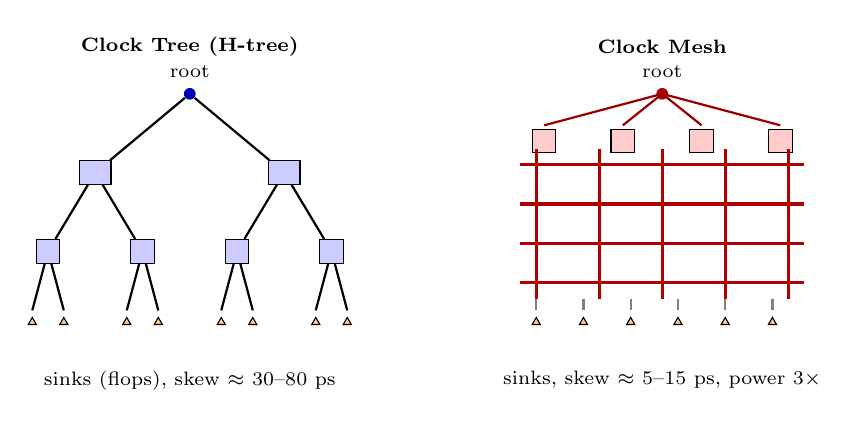
\begin{tikzpicture}[every node/.style={font=\scriptsize}]
  % ----- left: H-tree -----
  \begin{scope}[xshift=0cm]
    \node[font=\scriptsize\bfseries] at (2,4.2) {Clock Tree (H-tree)};
    \node[circle, fill=blue!70!black, inner sep=1.5pt, label=above:{root}] (r) at (2,3.6) {};
    \node[rectangle, draw, fill=blue!20, minimum width=4mm, minimum height=3mm] (b1) at (0.8,2.6) {};
    \node[rectangle, draw, fill=blue!20, minimum width=4mm, minimum height=3mm] (b2) at (3.2,2.6) {};
    \draw[thick] (r) -- (b1); \draw[thick] (r) -- (b2);
    \foreach \x/\name in {0.2/l1, 1.4/l2, 2.6/l3, 3.8/l4} {
      \node[rectangle, draw, fill=blue!20, minimum width=3mm, minimum height=3mm] (\name) at (\x,1.6) {};
    }
    \draw[thick] (b1) -- (l1); \draw[thick] (b1) -- (l2);
    \draw[thick] (b2) -- (l3); \draw[thick] (b2) -- (l4);
    \foreach \x in {0.0,0.4,1.2,1.6,2.4,2.8,3.6,4.0} {
      \node[regular polygon, regular polygon sides=3, draw, fill=orange!40, inner sep=0.6pt] at (\x,0.7) {};
    }
    \draw[thick] (l1) -- (0.0,0.85); \draw[thick] (l1) -- (0.4,0.85);
    \draw[thick] (l2) -- (1.2,0.85); \draw[thick] (l2) -- (1.6,0.85);
    \draw[thick] (l3) -- (2.4,0.85); \draw[thick] (l3) -- (2.8,0.85);
    \draw[thick] (l4) -- (3.6,0.85); \draw[thick] (l4) -- (4.0,0.85);
    \node[anchor=north, font=\scriptsize] at (2,0.2) {sinks (flops), skew $\approx$ 30--80~ps};
  \end{scope}

  % ----- right: mesh -----
  \begin{scope}[xshift=6cm]
    \node[font=\scriptsize\bfseries] at (2,4.2) {Clock Mesh};
    \node[circle, fill=red!70!black, inner sep=1.5pt, label=above:{root}] at (2,3.6) {};
    % drivers
    \foreach \x in {0.5,1.5,2.5,3.5} {
      \node[rectangle, draw, fill=red!20, minimum width=3mm, minimum height=3mm] at (\x,3.0) {};
      \draw[thick, red!60!black] (2,3.6) -- (\x,3.2);
    }
    % mesh grid
    \foreach \y in {1.2,1.7,2.2,2.7} {
      \draw[very thick, red!70!black] (0.2,\y) -- (3.8,\y);
    }
    \foreach \x in {0.4,1.2,2.0,2.8,3.6} {
      \draw[very thick, red!70!black] (\x,1.0) -- (\x,2.9);
    }
    % sinks
    \foreach \x in {0.4,1.0,1.6,2.2,2.8,3.4} {
      \node[regular polygon, regular polygon sides=3, draw, fill=orange!40, inner sep=0.6pt] at (\x,0.7) {};
      \draw[thick, gray] (\x,1.0) -- (\x,0.85);
    }
    \node[anchor=north, font=\scriptsize] at (2,0.2) {sinks, skew $\approx$ 5--15~ps, power 3$\times$};
  \end{scope}
\end{tikzpicture}
\caption{An H-tree (left) drives sinks through a fanout hierarchy of buffers; skew is moderate, power is moderate. A clock mesh (right) shorts together many parallel drivers across a metal grid so every sink sees nearly the same arrival time; skew is tiny, power and area are large.}
\label{fig:tree-vs-mesh}
\end{figure}

A \textbf{clock tree} (H-tree, fishbone, or balanced binary tree) drives sinks through a hierarchy of cloned buffers. CCOPT picks insertion points, sizes drivers, and balances branches. This is the default and it is what 95\% of blocks ship with.

A \textbf{clock mesh} shorts the outputs of many parallel drivers onto a metal grid, so every sink connects to a low-impedance plane that arrives at nearly the same time everywhere. Skew drops to single-digit picoseconds. \textbf{Power burns roughly 2--3$\times$} a comparable tree, because the grid is constantly switching and the parallel drivers all fight each other slightly. Mesh wins on multi-GHz CPU cores where 5~ps of skew determines the frequency the part hits. Tree wins on everything else.

Mesh is configured through a different family of CCOPT directives (mesh region, driver list, post-mesh tuning) and we will not unpack those here; the point is that the \textbf{same spec file} is the entry point for both worlds.

\begin{sidebar}
\textbf{What \texttt{ccopt\_design} actually does under the hood.} It is one Tcl command but the most computationally expensive single step in the flow, often hours on a large block. Internally it runs a sequence of passes: (1) \emph{clone} clock gates and buffers so fanout is balanced; (2) \emph{restructure} the logical hierarchy of the clock so latencies match across endpoints in the same skew group; (3) \emph{insert and size buffers} along the now-balanced topology; (4) \emph{legalize} placement after the inserted cells push neighbors around; (5) \emph{route} the clock nets with the declared NDR; (6) \emph{post-CTS optimize} data paths now that real clock latencies exist. Every one of those passes reads the CCOPT spec. Change one line in the spec and all six passes redo their work.
\end{sidebar}

\begin{figure}[h]
\centering
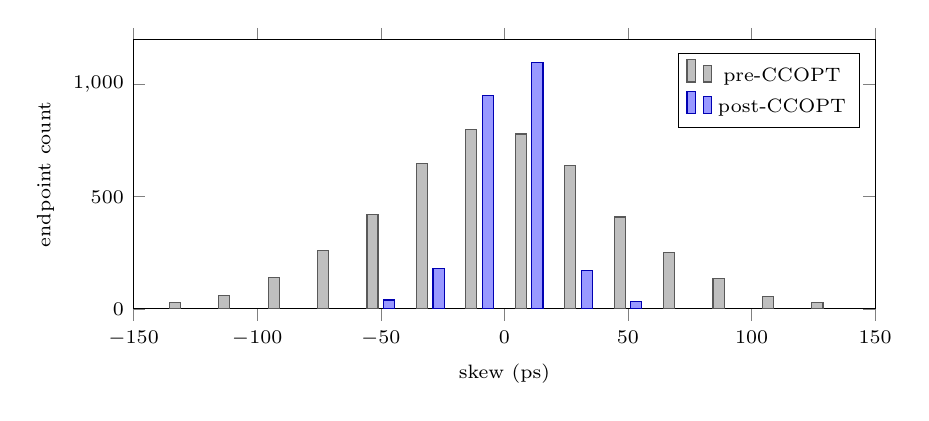
\begin{tikzpicture}
\begin{axis}[
  width=11cm, height=5cm,
  ybar, bar width=4pt,
  xlabel={skew (ps)}, ylabel={endpoint count},
  xmin=-150, xmax=150,
  ymin=0, ymax=1200,
  legend style={font=\scriptsize, at={(0.98,0.95)}, anchor=north east},
  tick label style={font=\scriptsize},
  label style={font=\scriptsize},
]
\addplot+[fill=gray!50, draw=gray!70!black] coordinates {
  (-130,30) (-110,60) (-90,140) (-70,260) (-50,420) (-30,650) (-10,800)
  (10,780) (30,640) (50,410) (70,250) (90,135) (110,55) (130,28)
};
\addlegendentry{pre-CCOPT}
\addplot+[fill=blue!40, draw=blue!70!black] coordinates {
  (-50,40) (-30,180) (-10,950) (10,1100) (30,170) (50,35)
};
\addlegendentry{post-CCOPT}
\end{axis}
\end{tikzpicture}
\caption{Endpoint skew distribution before and after \texttt{ccopt\_design} on a representative block. Pre-CTS the skew spread is essentially the placement-derived latency mismatch (often $\pm$130~ps). Post-CCOPT the distribution collapses to within the spec'd target skew (here 50~ps).}
\label{fig:skew-histogram}
\end{figure}

\begin{pdnote}{Why PD Cares}
\begin{itemize}
  \item \textbf{Arm Duc, your job right now.} Duc CTS work means you are reading CCOPT logs every day; understanding NDR enforcement order is the difference between debugging a clock spine in 20 minutes vs 2 hours. Same for skew groups: a generated clock dropped from the wrong group will produce cross-domain timing failures that look like SDC bugs and are actually a one-line CCOPT spec fix.
  \item \textbf{General PD engineer.} CTS is the only step where the tool builds new logic (clones buffers, inverters, gates) without you naming them in RTL. The spec is the contract that governs that creation; everything you do upstream (placement, floorplan) and downstream (route, sign-off) is reacting to what CCOPT decided.
  \item \textbf{VLSI interview.} ``What is useful skew, and when is it dangerous?'' is asked in roughly half of physical-design interviews. So is ``how do skew groups interact with generated clocks?'' Memorize the worked examples in this chapter and you will outscore most candidates.
\end{itemize}
\end{pdnote}

\begin{checkpoint}
You should now be able to (a) open a CCOPT spec and explain every \texttt{set\_ccopt\_property} line, (b) decide which clocks share a skew group and which do not, (c) compute the M5 track cost of a 2W2S NDR, (d) trade setup against hold with useful skew on a numerical path, and (e) know when mesh is worth its power bill.

\mnemonic{Spec the skew, shield the spine, borrow the slack.}
\end{checkpoint}

\chapter{Parasitic Files: ITF, the Mapping File, and SPEF}

\begin{tldr}
\begin{itemize}
  \item \textbf{Callback to Chapter 8 (CTS Spec):} Last chapter, the CTS spec told the tool how to build the clock. This chapter, parasitic files tell the tool (and the STA engine) what every wire it just built \emph{actually} does electrically.
  \item The \textbf{ITF} is the foundry's description of the metal stack: thicknesses, resistivities, dielectric constants. It is the source of truth for everything downstream.
  \item The \textbf{mapping file} bridges LEF/DEF layer names (\texttt{M3}, \texttt{VIA12}) to ITF layer indices. One typo here silently corrupts all RC.
  \item \textbf{SPEF} is the per net RC tree the extractor emits. Half of signoff timing debug is reading SPEF by hand.
\end{itemize}
\end{tldr}

\begin{hook}
The router placed an 80\,\textmu m wire on M3 between two flops. STA reports 47\,ps of delay on that net. Where did the 47 come from? Not from the cell. Not from the SDC. It came from a chain of files most engineers never open: a foundry ITF, a tiny mapping file, and a SPEF that the extractor cooked up at 3am during signoff. This chapter cracks that chain open.
\end{hook}

\section{ITF: The Interconnect Technology File}

The \textbf{ITF} (Interconnect Technology File) is a foundry deliverable that describes the back end of line stack exactly as the extraction engine sees it. Every metal layer has a thickness, a minimum width, a sheet resistance, and an etch profile. Every dielectric layer between metals has a thickness and a relative permittivity $\varepsilon_r$. Nothing in your timing comes out right if the ITF is wrong.

\begin{keyidea}
The ITF is not read by Innovus or PrimeTime directly. It is compiled by the foundry's extraction vendor (Synopsys StarRC, Cadence QRC) into a binary \textbf{TLU+} file or \textbf{QRC techfile}. That binary is what the extractor actually loads. The ITF is the human readable source; the TLU+ is the artifact your flow consumes.
\end{keyidea}

A small excerpt looks like this:

\begin{lstlisting}[style=eda,caption={ITF excerpt for a 7nm-ish stack.}]
TECHNOLOGY = my_7nm_stack
GLOBAL_TEMPERATURE = 25

CONDUCTOR M3 {
    THICKNESS    = 0.16
    WMIN         = 0.07
    SMIN         = 0.07
    RPSQ         = 0.072
    ETCH_VS_WIDTH { VALUES = (0.07, 0.005) (0.20, 0.008) }
}

DIELECTRIC ILD3 {
    THICKNESS = 0.20
    ER        = 2.7
}

DIELECTRIC ILD3_CAP {
    THICKNESS = 0.05
    ER        = 4.1   # nitride cap layer
}
\end{lstlisting}

Read it top down. M3 is 0.16\,\textmu m thick, the narrowest wire allowed is 70\,nm, the sheet resistance is 0.072\,$\Omega/\square$, and the etch shrinks the drawn width by a width dependent amount. Below M3 sits a 200\,nm ILD with $\varepsilon_r = 2.7$ (a low-k oxide), capped by a thin nitride layer at $\varepsilon_r = 4.1$. The extractor combines all of this with the actual routed geometry to produce R and C per segment.

\begin{hook}{The ITF is the stack's birth certificate}
The \textbf{foundry ships} an ITF that \textbf{freezes} the metal stack's electrical truth. Lose it, mis version it, or load the wrong corner, and \textbf{every SPEF downstream is fiction}.
\end{hook}

\begin{gut}
You see a TLU+ file in your flow but no ITF anywhere in the release. Is that normal? \gutans{Yes. Foundries often ship only the compiled TLU+ (and sometimes a redacted ITF) because the full ITF reveals proprietary process details. You consume the TLU+; you trust the foundry compiled it from the right ITF.}
\end{gut}

\section{The Mapping File: Tiny, Mission Critical}

The router speaks LEF/DEF layer names: \texttt{M1}, \texttt{M2}, \texttt{VIA12}. The ITF speaks its own layer indices and internal names. The \textbf{mapping file} (sometimes called the \texttt{nxtgrd} map, the \texttt{layer\_map}, or the \texttt{tech2itf} map) is the one line per layer dictionary that joins them.

\begin{lstlisting}[style=eda,caption={A tiny but mission critical mapping file.}]
# LEF/DEF name   ITF name      type
M1               METAL1        routing
M2               METAL2        routing
M3               METAL3        routing
VIA12            VIA1          via
VIA23            VIA2          via
\end{lstlisting}

If \texttt{M3} in the LEF is wrongly mapped to \texttt{METAL2} in the ITF, the extractor happily uses the thinner METAL2 thickness for every M3 segment in your design. Resistance is wrong by a constant factor. Capacitance is wrong by a different constant factor. Your STA looks clean. Silicon comes back broken.

\begin{pitfall}
A missing mapping line does \emph{not} always error out. Some flows fall back to a default layer or skip extraction on that layer entirely. You will see a warning buried in the extractor log and a SPEF that is missing parasitics on, say, every M7 net. Always grep the extraction log for \texttt{WARN} and \texttt{unmapped}.
\end{pitfall}

\section{SPEF: Where Parasitics Become a File You Read}

\textbf{SPEF} (Standard Parasitic Exchange Format) is the IEEE 1481 text format the extractor writes once per net. It contains the routed net's RC tree: every pin, every internal node (where a wire bends or branches), every R segment between nodes, and every C to ground (or coupling C to neighbor nets).

\move{1}{Set up the net.} Imagine a net \texttt{n42} driven by \texttt{U1/Y}, fanning out to two flop D pins, \texttt{FF1/D} and \texttt{FF2/D}. The router put down 80\,\textmu m of M3 total: 40\,\textmu m from the driver to a branch point, then 20\,\textmu m to each sink.

\move{2}{Compute the resistances.} M3 RPSQ is 0.072\,$\Omega/\square$. Wire width is 70\,nm, so squares per micron $= 1/0.07 \approx 14.3$. R per micron $= 14.3 \times 0.072 \approx 1.03\,\Omega/\text{\textmu m}$. So the 40\,\textmu m driver segment is $\sim 41\,\Omega$ and each 20\,\textmu m sink segment is $\sim 21\,\Omega$.

\move{3}{Compute the capacitances.} At 7nm M3 a sane total C is roughly 0.18\,fF/\textmu m (ground + coupling lumped). 40\,\textmu m $\to$ 7.2\,fF; 20\,\textmu m $\to$ 3.6\,fF. Split each segment's C into two lumps at its endpoints (the $\pi$ model the extractor uses).

\move{4}{Lay out the nodes.} Call them \texttt{1} (driver pin), \texttt{2} (branch), \texttt{3} (FF1/D), \texttt{4} (FF2/D). Caps lump at nodes 1, 2, 3, 4. Resistors sit between 1--2, 2--3, 2--4.

\move{5}{Pick the cap totals at each node.} Driver pin node 1 gets $\sim 3.6$\,fF from half of the driver segment. Branch node 2 gets the other half of the driver segment plus half of each sink segment: $3.6 + 1.8 + 1.8 = 7.2$\,fF. Sink nodes 3 and 4 each get the other half of their sink segment: $\sim 1.8$\,fF each, plus the pin cap of the receiving flop ($\sim 1.5$\,fF), total $\sim 3.3$\,fF.

\move{6}{Write it as SPEF.} See Listing~\ref{lst:spef-n42}.

\move{7}{Sanity check the totals.} Total wire C: $3.6 + 7.2 + 3.3 + 3.3 = 17.4$\,fF, close to the $0.18 \times 80 = 14.4$\,fF wire estimate plus $2 \times 1.5$\,fF pin caps. Total R from driver to FF1: $41 + 21 = 62\,\Omega$. Numbers feel right for 7nm M3.

\begin{lstlisting}[style=eda,caption={SPEF snippet for net \texttt{n42}. Reduced and slightly idealized.},label={lst:spef-n42}]
*SPEF "IEEE 1481-1999"
*DESIGN "duc_top"
*DATE "Mon May 26 14:02:11 2026"
*VENDOR "Cadence"
*PROGRAM "Quantus"
*VERSION "21.1"
*DESIGN_FLOW "PIN_CAP NONE" "FULL_CONNECTIVITY"
*DIVIDER /
*DELIMITER :
*BUS_DELIMITER [ ]
*T_UNIT 1 PS
*C_UNIT 1 FF
*R_UNIT 1 OHM
*L_UNIT 1 HENRY

*D_NET n42 17.4
*CONN
*I U1:Y O *L 0 *D BUFX4
*I FF1:D I *L 1.5 *D DFFX1
*I FF2:D I *L 1.5 *D DFFX1
*CAP
1 n42:1        3.6
2 n42:2        7.2
3 n42:3        3.3
4 n42:4        3.3
*RES
1 n42:1 n42:2  41.0
2 n42:2 n42:3  21.0
3 n42:2 n42:4  21.0
*END
\end{lstlisting}

\begin{figure}[h]
\centering
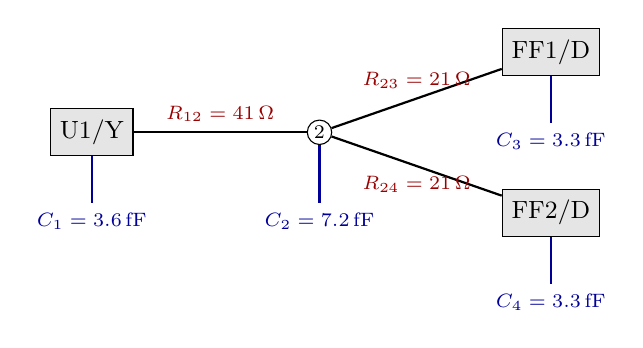
\begin{tikzpicture}[
  node distance=14mm,
  pin/.style={draw, fill=black!10, minimum size=6mm, font=\small},
  inode/.style={circle, draw, fill=white, inner sep=1pt, font=\scriptsize},
  capn/.style={font=\scriptsize, blue!60!black},
  res/.style={font=\scriptsize, red!60!black, midway, above}
]
  \node[pin] (d) {U1/Y};
  \node[inode, right=22mm of d] (n2) {2};
  \node[pin, above right=6mm and 22mm of n2] (s1) {FF1/D};
  \node[pin, below right=6mm and 22mm of n2] (s2) {FF2/D};

  \draw[thick] (d) -- node[res]{$R_{12}=41\,\Omega$} (n2);
  \draw[thick] (n2) -- node[res]{$R_{23}=21\,\Omega$} (s1);
  \draw[thick] (n2) -- node[res, below]{$R_{24}=21\,\Omega$} (s2);

  \draw[blue!60!black, thick] (d) -- ++(0,-9mm) node[capn, below]{$C_1=3.6$\,fF};
  \draw[blue!60!black, thick] (n2) -- ++(0,-9mm) node[capn, below]{$C_2=7.2$\,fF};
  \draw[blue!60!black, thick] (s1) -- ++(0,-9mm) node[capn, below]{$C_3=3.3$\,fF};
  \draw[blue!60!black, thick] (s2) -- ++(0,-9mm) node[capn, below]{$C_4=3.3$\,fF};
\end{tikzpicture}
\caption{RC tree for net \texttt{n42} reconstructed from the SPEF in Listing~\ref{lst:spef-n42}. Caps shown as lumps to ground; resistors between nodes.}
\label{fig:rc-tree}
\end{figure}

\begin{pausebox}
Before you read on, stare at Listing~\ref{lst:spef-n42} and Figure~\ref{fig:rc-tree} side by side. The \texttt{*CAP} section is just a list of (node, value) pairs. The \texttt{*RES} section is just (from, to, value). Once that clicks, SPEF stops being scary and becomes a circuit netlist you can sketch on paper in 60 seconds.
\end{pausebox}

\section{How STA Actually Uses SPEF}

The STA engine does \emph{not} simulate the RC tree as a SPICE deck (way too slow for millions of nets). It reduces the tree to an \textbf{effective capacitance} $C_{\text{eff}}$ seen by the driver and an \textbf{Elmore delay} (or higher order moment) to each sink. CCS and ECSM models then use $C_{\text{eff}}$ to pick the right driver waveform from the \texttt{.lib}.

The \textbf{Elmore delay} to a sink is the sum, over every resistor $R_i$ on the path from driver to sink, of $R_i$ times the total downstream capacitance hanging off $R_i$.

\begin{hook}{Elmore = R times all the C it sees downstream}
For each \textbf{resistor on the path}, \textbf{multiply it by every cap downstream} of it, \textbf{sum the products}. Skip a downstream branch and your delay is wrong by the branch's contribution.
\end{hook}

Worked example for the path \texttt{U1/Y} $\to$ \texttt{FF1/D} in Figure~\ref{fig:rc-tree}:

\begin{itemize}
  \item $R_{12} = 41\,\Omega$ sees everything downstream of node 2: $C_2 + C_3 + C_4 = 7.2 + 3.3 + 3.3 = 13.8$\,fF.
  \item $R_{23} = 21\,\Omega$ sees only $C_3 = 3.3$\,fF.
\end{itemize}

$$ t_{\text{Elmore}} = 41 \times 13.8 + 21 \times 3.3 = 565.8 + 69.3 = 635.1\,\Omega\cdot\text{fF} = 0.635\,\text{ps}.$$

That is the \emph{wire delay} contribution at sink FF1/D. The driver's intrinsic delay (from the \texttt{.lib}, evaluated at the effective load) is added on top. The 47\,ps from the chapter opener is mostly the driver, with a small contribution from this Elmore term. Now you know where it came from.

\begin{gut}
If the router rerouted node 2 farther from the driver, doubling $R_{12}$ to 82\,$\Omega$, what happens to FF1's Elmore delay? \gutans{The first term doubles: $82 \times 13.8 = 1131.6$. Total becomes $1131.6 + 69.3 = 1200.9\,\Omega\cdot\text{fF} \approx 1.2$\,ps. The shared resistor near the driver dominates because it sees the entire downstream capacitance.}
\end{gut}

\section{SPEF Flavors and Corners}

SPEF is not a single file. The extractor emits one SPEF \emph{per RC corner}, and modern signoff loads them all under MMMC. The standard set is:

\begin{itemize}
  \item \textbf{Cworst}: worst case coupling cap. Used for setup analysis when long wires hurt the most.
  \item \textbf{Cbest}: best case (lowest) cap. Used for hold analysis where fast nets cause race conditions.
  \item \textbf{RCworst}: worst R \emph{and} worst C. Pessimistic for setup on resistive paths.
  \item \textbf{RCbest}: best R and best C. Optimistic; hold analysis on long wires.
  \item \textbf{Typical}: nominal corner for sanity and reporting.
\end{itemize}

\begin{figure}[h]
\centering
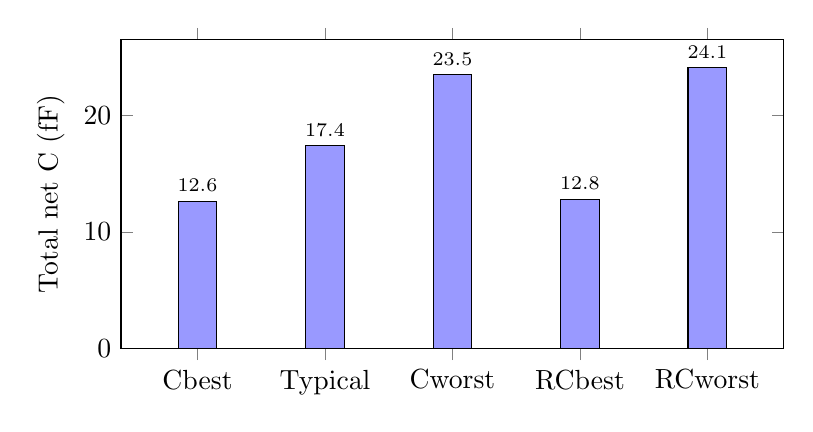
\begin{tikzpicture}
\begin{axis}[
  width=10cm, height=5.5cm,
  ybar, bar width=14pt,
  ylabel={Total net C (fF)},
  symbolic x coords={Cbest, Typical, Cworst, RCbest, RCworst},
  xtick=data, ymin=0,
  nodes near coords, nodes near coords style={font=\scriptsize},
  enlarge x limits=0.15,
]
\addplot[fill=blue!40] coordinates {
  (Cbest, 12.6) (Typical, 17.4) (Cworst, 23.5) (RCbest, 12.8) (RCworst, 24.1)
};
\end{axis}
\end{tikzpicture}
\caption{Extracted total C for net \texttt{n42} across the five RC corners. The same net, the same routing, five different SPEFs.}
\label{fig:corners}
\end{figure}

Five SPEFs per scenario. Multiply by your PVT corners, modes, and OCV settings, and the MMMC explosion from the back matter chapter stops being abstract: at Arm signoff you can easily be loading 40+ SPEFs in a single \texttt{create\_analysis\_view} grid.

\begin{pitfall}
Comparing the C of a net across two SPEFs and concluding "extraction is broken" is a classic rookie mistake. Check the header. If one is \texttt{*DESIGN\_FLOW "..."} Cworst and the other is Cbest, they are \emph{supposed} to differ by 30 to 50 percent. They are not the same file.
\end{pitfall}

\begin{sidebar}{DSPF vs SPEF vs SBPF}
\textbf{DSPF} (Detailed Standard Parasitic Format) is the older, Synopsys originated format. It preserves every internal node with explicit names like \texttt{n42:1234}, making it easy to map back to physical geometry. SPICE simulators love it. \textbf{SBPF} (Synopsys Binary Parasitic Format) is a compressed binary form for huge designs.

\textbf{SPEF} won as the lingua franca because IEEE standardized it, every vendor reads it, and it supports name mapping (\texttt{*NAME\_MAP}) to compress the file. Some analog teams still ship DSPF for block level SPICE sims, then the digital flow converts to SPEF for STA. At Arm you will mostly see SPEF; DSPF shows up only when a memory or analog macro hands you their extracted view.
\end{sidebar}

\begin{pdnote}{Why PD Cares about Parasitic Files}
\begin{itemize}
  \item \textbf{At Arm on Duc:} you will be staring at SPEF when a path mysteriously misses timing at signoff that was clean post route. Learning to grep \texttt{*D\_NET <netname>} out of a 4\,GB SPEF, sketch the RC tree, and hand compute Elmore is a core Innovus debugging skill. The first time a senior engineer asks "what's the Reff on the second branch?" you want to know exactly which lines to look at.
  \item \textbf{Generic PD engineer:} parasitic correlation between extractor outputs and silicon is one of the top three reasons a tapeout slips. If your team upgrades TLU+ mid project, every block's timing changes and you have to re-close. Understanding what an ITF, mapping file, and SPEF \emph{are} is the prerequisite to even having that conversation.
  \item \textbf{VLSI interview:} "Walk me through how a wire becomes a delay number in STA" is a standard question. The answer (geometry $\to$ ITF $\to$ TLU+ $\to$ extractor $\to$ SPEF $\to$ reduction $\to$ Elmore $\to$ .lib lookup) is what this chapter is about. Saying "the tool just figures it out" is a fast way to end the interview.
\end{itemize}
\end{pdnote}

\begin{checkpoint}
\mnemonic{ITF cooks the stack, the map joins the names, SPEF tells STA what the wire really is.}

You should now be able to:
\begin{itemize}
  \item Explain why the ITF lives upstream of TLU+ and never goes into Innovus directly.
  \item Read a five line mapping file and name what breaks if a line is missing.
  \item Sketch an RC tree from a \texttt{*D\_NET} block in a SPEF in under a minute.
  \item Compute Elmore delay to any sink given the tree.
  \item Name the five standard RC corners and which analysis each one feeds.
\end{itemize}
\end{checkpoint}

\chapter{What Changes in the Real World}

\begin{tldr}
\begin{itemize}
  \item \textbf{Last chapter:} parasitic files (ITF, mapping, SPEF) told the tool what each routed wire actually does electrically. \textbf{This chapter:} we zoom out and see how every input covered so far explodes in production: MMMC view counts, pin access, derate models, and DEF size growth through the flow.
  \item \textbf{MMMC is multiplication, not addition.} Five cell families times three voltages times three temperatures times six process corners times four modes is not a clever rhetorical flourish; it is a literal \texttt{.lib} count north of one thousand.
  \item \textbf{Pin access is the new floorplan.} At 7\,nm, an instance can be DRC-clean in placement and still strand the router because the M1 pin geometry offers too few via-cut candidates.
  \item \textbf{OCV, AOCV, POCV change the answer on the same SDC.} A path that meets timing at 1.05\,ns with AOCV can fail at 1.10\,ns with flat OCV without a single edit to the constraint file.
\end{itemize}
\end{tldr}

\begin{hook}
A junior engineer hands you a netlist, a tech file, an SDC, a LEF, a Liberty, and a DEF. You set up the run. The tool refuses to launch. The error is one line: \texttt{ERROR: analysis\_view 'func\_ss\_0p72\_125c\_setup' references missing delay\_corner}. You did not forget a file. You forgot that the toy version of every input you just read about explodes into a matrix of views the moment the block is real. So what does the matrix actually look like, and where does the explosion bite first?
\end{hook}

% =====================================================================
\section{MMMC: the Liberty view explosion}
% =====================================================================

The toy mental model says ``load a \texttt{.lib}, load an SDC, run STA.'' The production model says ``enumerate every physically possible combination of process, voltage, temperature, cell flavor, and operating mode, then promise the foundry your design works at every cross product.'' That promise is what \textbf{MMMC} (Multi-Mode Multi-Corner) signoff actually encodes.

\subsection{Counting the Liberty views directly}

Walk through it with the numbers in front of you. The arithmetic is boring; the size of the answer is not.

\move{1} \textbf{Cell families.} A modern 7\,nm-class standard cell library ships in five threshold flavors: \textbf{RVT, LVT, HVT, ULVT, ELVT}. That is \textbf{5}.

\move{2} \textbf{Voltages.} Each flavor is characterized at \textbf{nominal, low, and overdrive}. That is \textbf{3}.

\move{3} \textbf{Temperatures.} Automotive-aware blocks characterize at \textbf{$-40^\circ$C, $25^\circ$C, $125^\circ$C}. That is \textbf{3}.

\move{4} \textbf{Process corners.} Setup signoff uses \textbf{SS, FF, TT, SF, FS}, and hold typically demands a second \textbf{FS variant} with a separate skew assumption. That is \textbf{6}.

\move{5} \textbf{Operating modes.} The block runs in \textbf{functional, scan-shift, scan-capture, and retention} modes. That is \textbf{4}.

\move{6} \textbf{Multiply.} $5 \times 3 \times 3 \times 6 \times 4 = \mathbf{1080}$ Liberty views. The chapter's old ``easily exceeds 200'' was a comforting understatement.

\move{7} \textbf{Wall-clock cost.} Liberty parsing scales roughly linearly. At \textbf{30 seconds per view}, parsing alone is $1080 \times 30 = 32{,}400$ seconds, or \textbf{nine hours} if you do it serially. In practice tools cache and parallelize, but the order of magnitude is real, and every parse hits disk.

\begin{keyidea}
The MMMC view count is the \textbf{product} of every characterization axis, not the sum. Adding a single new voltage point does not add one view; it multiplies the entire existing matrix by a new factor.
\end{keyidea}

\subsection{How Innovus actually structures it}

Innovus does not consume 1080 raw Liberty files as 1080 independent things. It organizes them into three objects that compose:

\begin{itemize}
  \item \textbf{library\_set}: a bundle of \texttt{.lib} files that belong together (one PVT corner across all cell families).
  \item \textbf{delay\_corner}: a library\_set plus an RC corner (the QRC tech file) plus an OCV derate spec.
  \item \textbf{constraint\_mode}: an SDC file plus the mode it represents (functional, scan, retention).
  \item \textbf{analysis\_view}: the actual scenario you sign off, formed by pairing one \texttt{constraint\_mode} with one \texttt{delay\_corner}.
\end{itemize}

The number that matters at runtime is not the 1080 Liberty views; it is the \textbf{number of analysis\_views you activate}. A typical 7\,nm block runs signoff on roughly \textbf{20 to 40 active views} simultaneously, picked from the full matrix to cover worst setup, worst hold, worst leakage, and the mode-specific corners. The full 1080 is the universe; the active set is the working slice.

\begin{hook}
\textbf{The Liberty matrix is a warehouse, the analysis\_view list is the loading dock.} If you forget which crates you actually shipped today, signoff signs off on the wrong block and the tapeout slips a month.
\end{hook}

\begin{gut}
A block uses 4 cell families, 2 voltages, 2 temperatures, 5 process corners, and 3 modes. How many Liberty views, and how is the \emph{analysis\_view} number different from that?
\gutans{$4 \times 2 \times 2 \times 5 \times 3 = 240$ Liberty views. The analysis\_view count is whatever subset of (constraint\_mode $\times$ delay\_corner) you actually activate for signoff, typically 15 to 30 in production. The matrix sizes the disk; the active list sizes the runtime.}
\end{gut}

% =====================================================================
\section{Pin access: when LEF stops being enough}
% =====================================================================

At 28\,nm, a standard cell's LEF \texttt{PIN} section drew an M1 rectangle spanning the cell width. The router saw a long target, dropped a via almost anywhere along it, and moved on. At 7\,nm that same geometry strands the router, and placement legality stops implying routability.

\subsection{Why the 28\,nm pin shape fails at 7\,nm}

\move{1} \textbf{Track pitch.} A 7\,nm M1 routing pitch is roughly \textbf{36\,nm}. The router can only place a wire on one of those tracks; nothing in between is legal.

\move{2} \textbf{Pin geometry must land on a track.} A pin rectangle whose center sits between two tracks is invisible to the router. The cell can be placed, but no legal wire can touch it.

\move{3} \textbf{Via cuts are quantized.} A 7\,nm V1 cut is roughly $32 \times 32$\,nm and must obey same-cut spacing. A pin shape that is only \textbf{one track wide} offers \textbf{one via candidate}. If that candidate clashes with a neighbor cell's via, the router has zero alternatives.

\move{4} \textbf{Multi-access pins.} Modern foundry cell libraries require each input pin to offer at least \textbf{two non-conflicting via candidates}, sometimes three. This is enforced by a separate deliverable.

\move{5} \textbf{Pin access models.} The foundry ships a \textbf{pin access model} (often a CSV or proprietary table per cell) listing which access points are usable under which neighbor contexts. It augments the LEF; it does not replace it.

\begin{figure}[h]
\centering
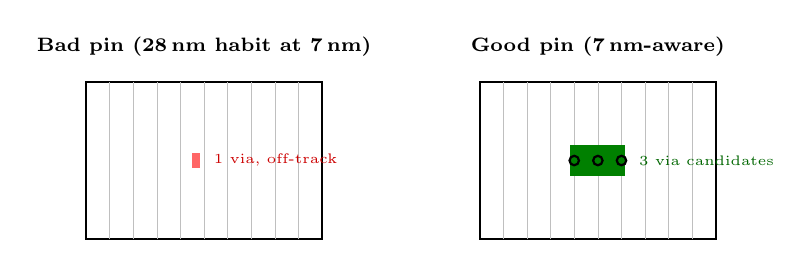
\begin{tikzpicture}[font=\scriptsize]
  % BAD pin
  \begin{scope}
    \node[anchor=south, font=\scriptsize\bfseries] at (1.5,2.2) {Bad pin (28\,nm habit at 7\,nm)};
    % cell outline
    \draw[thick] (0,0) rectangle (3,2);
    % tracks
    \foreach \x in {0.3,0.6,0.9,1.2,1.5,1.8,2.1,2.4,2.7} {
      \draw[gray!50, very thin] (\x,0) -- (\x,2);
    }
    % pin shape (between tracks, narrow)
    \fill[red!60] (1.35,0.9) rectangle (1.45,1.1);
    \node[red!80!black, anchor=west, font=\tiny] at (1.5,1.0) {1 via, off-track};
  \end{scope}

  % GOOD pin
  \begin{scope}[xshift=5cm]
    \node[anchor=south, font=\scriptsize\bfseries] at (1.5,2.2) {Good pin (7\,nm-aware)};
    \draw[thick] (0,0) rectangle (3,2);
    \foreach \x in {0.3,0.6,0.9,1.2,1.5,1.8,2.1,2.4,2.7} {
      \draw[gray!50, very thin] (\x,0) -- (\x,2);
    }
    % pin spans three tracks, on-grid
    \fill[green!50!black] (1.15,0.8) rectangle (1.85,1.2);
    \foreach \x in {1.2,1.5,1.8} {
      \draw[black, thick] (\x,1.0) circle (0.06);
    }
    \node[green!40!black, anchor=west, font=\tiny] at (1.9,1.0) {3 via candidates};
  \end{scope}
\end{tikzpicture}
\caption{Pin access geometry at 7\,nm. The left pin is on-grid for placement but off-grid for routing tracks and offers a single via candidate; the router has no fallback when the neighbor cell wants the same cut. The right pin spans three tracks and offers three independent via candidates.}
\end{figure}

\begin{pitfall}
``Placement DRC clean'' at 7\,nm does \textbf{not} mean ``routable.'' A block can finish placement with zero violations and then accumulate thousands of \textbf{unconnected nets} in detail route because of pin-access conflicts the placer never modeled. Always check the pin-access report before signing off on a placement milestone.
\end{pitfall}

% =====================================================================
\section{AOCV and POCV: same SDC, different answer}
% =====================================================================

The SDC defines the constraints. The derate model defines how pessimistic the tool is when it applies those constraints. Three derate models dominate production today: \textbf{flat OCV}, \textbf{AOCV} (Advanced OCV, depth-aware), and \textbf{POCV} (Parametric OCV, statistical).

\subsection{Worked example: a 12-level path at 1.0\,ns nominal}

The path has \textbf{12 logic levels} (12 cells on the data path between launch and capture flops). Nominal cell-plus-net delay sums to \textbf{1.0\,ns}. The clock period is 1.05\,ns.

\move{1} \textbf{Flat OCV.} The launch path is derated up by 1.10, the capture path down by 0.90. Launch delay becomes $1.0 \times 1.10 = \mathbf{1.10\,\text{ns}}$. With a 1.05\,ns period the path \textbf{misses by 50\,ps}.

\move{2} \textbf{AOCV table lookup.} The AOCV table is depth-dependent: \textbf{1.15} at depth 1, \textbf{1.05} at depth 12, with linear interpolation between. The longer the path, the less pessimism, because statistical variation of independent stages partially cancels.

\move{3} \textbf{AOCV applied.} At depth 12 the multiplier is \textbf{1.05}. Launch delay is $1.0 \times 1.05 = \mathbf{1.05\,\text{ns}}$. The path \textbf{just meets} the 1.05\,ns period.

\move{4} \textbf{POCV per-cell sigma.} Each cell publishes a $\sigma/\mu$ ratio in a \texttt{.lib} extension. Assume the 12 cells contribute equal mean delay (83.3\,ps each) and each has $\sigma/\mu = 0.05$. Per-cell $\sigma = 0.05 \times 83.3 = 4.17$\,ps.

\move{5} \textbf{POCV sqrt-sum-of-squares.} Path $\sigma = \sqrt{12 \times 4.17^2} = \sqrt{208.7} = \mathbf{14.4\,\text{ps}}$. The path mean is 1.000\,ns.

\move{6} \textbf{POCV signoff (mean + $3\sigma$).} Launch delay is $1.000 + 3 \times 0.0144 = 1.000 + 0.043 = \mathbf{1.043\,\text{ns}}$. The path meets with \textbf{7\,ps of margin}, more than AOCV gave you.

\move{7} \textbf{Tally.}
\begin{itemize}
  \item Flat OCV: 1.10\,ns, \textbf{fails by 50\,ps}.
  \item AOCV: 1.05\,ns, \textbf{meets by 0\,ps}.
  \item POCV: 1.043\,ns, \textbf{meets by 7\,ps}.
\end{itemize}

Same SDC. Same netlist. Same instance placement. Three different signoff verdicts because the derate engine changed.

\begin{pausebox}
Halfway recap. MMMC says ``how many corners.'' Pin access says ``can the router even reach.'' OCV/AOCV/POCV says ``how mean is the signoff math.'' All three modify outputs the SDC and Liberty already promised, so the toy mental model of ``one .lib, one SDC, one answer'' is a story the production flow does not tell.
\end{pausebox}

\begin{gut}
The same 12-level path under flat OCV fails by 50\,ps; under POCV it passes with 7\,ps margin. Did the silicon get faster?
\gutans{No. The silicon did not change. The \textbf{statistical model of how variation accumulates} changed. Flat OCV assumes every stage hits its worst case simultaneously, which becomes wildly pessimistic as path depth grows; POCV models that independent stages partially cancel and reports a tighter, more physically realistic margin.}
\end{gut}

% =====================================================================
\section{DEF growth through the flow, with post-CTS as the surprise}
% =====================================================================

DEF is the same file format at every PD checkpoint, but the byte count tells a story about what each stage added. The post-CTS jump is the one new engineers miss, because the netlist itself changed underneath them.

\subsection{Worked example: a 1M-instance block}

Take a 1\,million-instance block and follow the DEF through the flow.

\move{1} \textbf{Post-floorplan.} DEF holds \texttt{DIEAREA}, \texttt{ROWS}, IO pin placement, and macro placement. Standard cells are not placed; \texttt{COMPONENTS} lists them with placeholder status. Size: \textbf{$\sim$30\,MB}.

\move{2} \textbf{Post-place.} Every one of the 1\,M instances now has an \texttt{(x, y)} coordinate and an orientation. Each \texttt{COMPONENT} line grows by roughly 40\,bytes. Net topology has not been written yet. Size: \textbf{$\sim$80\,MB}.

\move{3} \textbf{Post-CTS.} The CTS engine \textbf{inserted new instances}, roughly \textbf{5\% of the original count}, as clock buffers, inverters, and ICGs. That is \textbf{50\,000 new components}. It also \textbf{rewrote every clock \texttt{NET}} to reflect the new tree topology. Size: \textbf{$\sim$120\,MB}.

\move{4} \textbf{Post-route.} Every \texttt{NET} now carries full routing geometry: \texttt{ROUTED} segments with layer, coordinates, and via instances. Average net contributes 200 to 400 bytes of geometry. Size: \textbf{$\sim$350\,MB}.

\move{5} \textbf{The post-CTS diff is the most informative diff in the flow.} Run \texttt{diff post\_place.def post\_cts.def}. The only changes you should see are (a) new clock-buffer \texttt{COMPONENT} entries and (b) rewritten clock \texttt{NET} entries. If you see signal nets change, CTS touched something it should not have.

\begin{figure}[h]
\centering
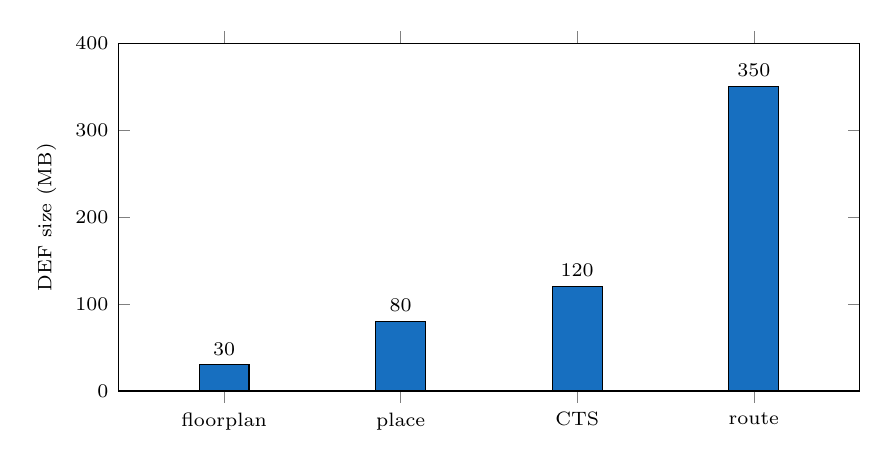
\begin{tikzpicture}
\begin{axis}[
  width=11cm, height=6cm,
  ybar,
  bar width=18pt,
  ylabel={DEF size (MB)},
  symbolic x coords={floorplan, place, CTS, route},
  xtick=data,
  nodes near coords,
  nodes near coords style={font=\scriptsize},
  ymin=0, ymax=400,
  enlarge x limits=0.2,
  tick label style={font=\scriptsize},
  label style={font=\scriptsize},
]
\addplot[fill=cyan!50!blue, draw=black] coordinates {(floorplan,30) (place,80) (CTS,120) (route,350)};
\end{axis}
\end{tikzpicture}
\caption{DEF size growth across PD stages for a 1\,M-instance 7\,nm block. The post-place to post-CTS jump (+40\,MB) reflects 50\,000 inserted clock instances and rewritten clock NETs. The post-route jump (+230\,MB) is dominated by per-net routing geometry.}
\end{figure}

\begin{hook}
\textbf{The post-CTS DEF gains 40\,MB and 50\,000 instances overnight; if you do not diff it against post-place, you will not notice when CTS quietly buffered a signal net and your scan chain breaks at silicon.}
\end{hook}

\begin{sidebar}
Why does the post-route jump dwarf everything else? Because routing geometry is the only DEF content that scales with \textbf{net length in microns}, not with \textbf{instance count}. A single long bus net on M5 can contribute as much DEF text as a hundred short local nets. This is also why \texttt{def2stream} for GDS conversion is the slowest step in the back-end: it is parsing geometry, not instances.
\end{sidebar}

% =====================================================================
\section{Why PD Cares}
% =====================================================================

\begin{pdnote}[Why PD Cares]
\textbf{Arm PD intern lens (you, this summer on Duc):} you will load MMMC views in your first week, and the first error will be a missing \texttt{analysis\_view} reference in the Innovus setup script. Knowing that \texttt{analysis\_view = constraint\_mode $\times$ delay\_corner} is what unblocks you in fifteen minutes instead of two days. You will also spend serious time staring at post-CTS DEF diffs because Duc is CTS-heavy.\\
\textbf{Generic PD engineer lens:} when a tool ``runs out of memory'' or ``hangs on STA setup,'' the answer is almost always MMMC scenario explosion or a derate file mismatch, not an algorithmic regression. Check the view count first.\\
\textbf{VLSI interview lens:} expect ``what is the difference between OCV, AOCV, and POCV, and when would you use each?'' as a standard signoff-flow question. The right answer leads with the numbers (flat is most pessimistic, POCV is least pessimistic on long paths) and then names the formulas.
\end{pdnote}

% =====================================================================
\begin{checkpoint}
Production PD warps four inputs around the toy mental model: Liberty views \textbf{multiply}, pins must \textbf{align}, derate \textbf{rewrites the verdict}, and DEF \textbf{grows fastest at CTS and route}.
\mnemonic{Multiply, Align, Derate, Grow (MADG).}
\end{checkpoint}


% =====================================================================
% BACK MATTER
% =====================================================================

\chapter{Common Mistakes}

A numbered list, intentionally short. Every one of these is something a PD intern (or interviewer) has actually seen.

\begin{enumerate}[leftmargin=*]
  \item \textbf{Loading the wrong .lib corner} and wondering why the design closes timing at the typical corner but blows up at SS. The .lib loaded is not the corner you think.
  \item \textbf{Cell name mismatch} between synthesized netlist and the .lib (cell renamed across library versions, or wrong library swapped in). PD throws missing-reference errors before floorplan even starts.
  \item \textbf{Forgetting to define a generated clock}, so STA reports timing on a phantom unconstrained clock and the slack looks fine when it is silently meaningless.
  \item \textbf{Using \texttt{set\_false\_path} as a hammer} to make a violating endpoint go away. The path is still real in silicon; you just stopped checking it.
  \item \textbf{Pin geometry off the routing grid} in cell LEF. The placer is happy. The router cannot connect.
  \item \textbf{Confusing tech file with tech-LEF.} They overlap. They are not identical. Tools differ in which they consume.
  \item \textbf{Comparing DEF coordinates raw} without honoring \texttt{UNITS DISTANCE MICRONS}. A coordinate of 12500 is 12.5\,\textmu m at scale 1000 and 6.25\,\textmu m at scale 2000.
  \item \textbf{Skipping the MMMC scenarios at intermediate PD stages} and only running full MMMC at signoff. Late surprises are the most expensive surprises.
  \item \textbf{Treating LEF and DEF as the same thing.} LEF is library (abstract cell views). DEF is design (this design's instances and their placement).
  \item \textbf{Editing the netlist by hand} late in the flow to ``fix'' something. Synthesis owns the netlist. Hand-edits diverge from RTL and create ECO chaos at signoff.
\end{enumerate}

% =====================================================================
\chapter{Interview-Ready 90-Second Answer}

\textbf{The setup.} An interviewer says: \textit{``Walk me through the inputs a Physical Design tool needs to start a job, and what each one contributes.''} You have ninety seconds. Cover the italicized block below with your hand. Recite your version out loud. Then uncover and compare.

\bigskip
\begin{quote}\itshape
A PD tool needs nine inputs. Three are static descriptions of the parts (\textbf{netlist}, \textbf{.lib}, \textbf{LEF}), three are constraints on what the result must satisfy (\textbf{SDC}, \textbf{tech file}, \textbf{CTS spec}), and three are state that gets written and re-read across the flow (\textbf{DEF}, \textbf{ITF/mapping}, \textbf{SPEF}). The \textbf{netlist} is the gate-level graph: cell instances, nets, and top-level ports. The \textbf{.lib} stores cell behavior as \textbf{NLDM lookup tables} indexed by input slew and output load, bilinearly interpolated at runtime, and at advanced nodes it stores \textbf{CCS} time-varying current waveforms so Miller capacitance and receiver-pin nonlinearity aren't averaged away. The \textbf{LEF} (cell LEF plus tech-LEF) is the physical abstraction so the placer and router never have to open GDS. The \textbf{SDC} is the Tcl timing contract: clocks, IO delays, uncertainty, false paths, multicycles. The \textbf{technology file} is the foundry rulebook for layer widths, spacings, vias, and multi-patterning colors. The \textbf{CTS spec} (CCOPT spec for Innovus) is the declarative description of how the clock network gets built: skew targets, NDR rules, useful-skew limits, and skew groups. The \textbf{DEF} is the physical state, emitted at every checkpoint; the DEF grows roughly 30 MB post-floorplan, 80 MB post-place, 120 MB post-CTS once CCOPT inserts roughly 5\% more instances as clock buffers, and 350 MB post-route for a 1M-instance block. \textbf{ITF} plus the \textbf{mapping file} feed the extractor, which emits \textbf{SPEF} (one per RC corner) describing every wire's actual R and C. STA then reads the SPEF, builds Elmore or CCS-aware delays, and reports slack against the SDC. Across MMMC the .lib and SPEF counts multiply: five cell families times three voltages times three temperatures times six corners times four modes lands at over a thousand views, which is why a real signoff run is a coffee break, not a click. The shape of the whole picture: netlist tells you what to build, SDC plus CTS spec tell you how fast and how clean the clock must be, .lib plus LEF plus tech file tell you what is physically and electrically legal, DEF records where everything landed, and ITF plus SPEF say what each routed wire actually does. That is the PD pipeline in ninety seconds.
\end{quote}

% =====================================================================
\chapter{Cumulative Recall Sheet}

Every chapter compressed to its Key Idea and mnemonic. One page. Use it as your spaced-repetition surface. If you can read this page and rebuild the rest of the book from it, the book has done its job.

\bigskip

\begin{tabular}{@{}p{0.06\linewidth} p{0.66\linewidth} p{0.22\linewidth}@{}}
\toprule
\textbf{Ch.} & \textbf{Key Idea} & \textbf{Mnemonic} \\
\midrule
1 & PD is not one tool eating one file. It is a pipeline of engines (synthesis hand-off, floorplan, placement, CTS, route, signoff) where each engine demands a specific input no other input can substitute for. Lose one, lose that engine. & NSL-LTD \\
\addlinespace
2 & A netlist is a graph of cell instances connected by nets, with top-level ports as the only opening to the outside world. Everything PD does (placement, routing, timing) operates on this graph. & INP \\
\addlinespace
3 & A timing library is a characterized lookup of cell behavior across PVT corners. NLDM boils each cell's delay into a 2D table indexed by input slew and output load; the tool bilinearly interpolates between grid points. & Slew in, load out \\
\addlinespace
4 & The LEF is the contract between the cell library and the placer/router. It promises footprint, pin layers, and blockages so the tool can resolve placement and routing without ever opening the GDS. & SIZE, SITE, PIN, OBS \\
\addlinespace
5 & The SDC is the single source of truth that converts a netlist into a timed promise. Every downstream tool (synthesis, STA, PnR, signoff) measures success against the same clocks, IO delays, uncertainties, and exceptions. & Setup early, hold late \\
\addlinespace
6 & The technology file is the foundry rulebook that names every physical layer, fixes its geometric and electrical parameters, and tells the PD tool exactly which shapes it is allowed to draw. & LIVR-C \\
\addlinespace
7 & A DEF file is a textual snapshot of the design's physical state at one point in the PD flow. LEF describes cells in the abstract; DEF describes this design's instances in concrete coordinates. & DRCPN \\
\addlinespace
8 & The CTS spec is the only place in the flow where you express clock-network intent declaratively; everything else (placement, route, signoff) just reacts to the tree CCOPT builds from it. & Spec skew, shield spine, borrow slack \\
\addlinespace
9 & Parasitic files are a three-stage pipeline: ITF describes the process to the extractor, the mapping file binds LEF/DEF layer names to ITF indices, and SPEF records what every wire actually does electrically (R, C, coupling) per RC corner for STA. & ITF cooks, map joins, SPEF tells \\
\addlinespace
10 & MMMC view count is the product of every characterization axis, not the sum. Adding one new voltage point does not add one view; it multiplies the entire existing matrix by a new factor. & MADG \\
\bottomrule
\end{tabular}

% =====================================================================
\chapter{Practice Problems}

Mixed difficulty. Mixed type. Mixed chapter. The order is \textbf{intentionally interleaved}; do not skip around to cluster by topic. Interleaved retrieval beats blocked practice roughly two to one on retention (Rohrer and Taylor).

\section*{Problem 1 (Ch.~5 numerical, setup slack)}
Given clock period $T = 2\,\text{ns}$, combinational delay $D = 1.6\,\text{ns}$, clock skew $= -0.05\,\text{ns}$, setup time of capture flop $T_s = 0.12\,\text{ns}$, and clock uncertainty $U = 0.10\,\text{ns}$. Compute setup slack. Then with $D_{\min} = 0.15\,\text{ns}$ and $T_h = 0.04\,\text{ns}$, compute hold slack. Which check fails?

\section*{Problem 2 (Ch.~1 conceptual, missing input triage)}
A PD bring-up script fails on the message \texttt{ERROR: cannot resolve cell NAND2\_X1}. List the input files where the root cause could live, and for each, state the one debugging command you would run first.

\section*{Problem 3 (Ch.~3 numerical, NLDM bilinear interpolation)}
Given a $3\times3$ NLDM \texttt{cell\_fall} table with input slews $\{30, 80, 200\}$ ps and output loads $\{4, 12, 25\}$ fF, with delay values:
\[
\begin{array}{c|ccc}
 & 4\,\text{fF} & 12\,\text{fF} & 25\,\text{fF} \\
\hline
30 & 35 & 60 & 95 \\
80 & 55 & 85 & 130 \\
200 & 110 & 160 & 220 \\
\end{array}
\quad \text{(ps)}
\]
Compute fall delay for slew $= 60$ ps and load $= 18$ fF. Show all four corner samples and both interpolation passes.

\section*{Problem 4 (Ch.~4 + Ch.~6, grid-and-pitch arithmetic)}
A tech-LEF declares M2 with \texttt{DIRECTION VERTICAL PITCH 0.14} and track offset 0. A cell-LEF gives PIN A as \texttt{RECT 0.10 0.40 0.13 0.80} on M2. Does pin A land on a routing track? If not, what is the smallest shift in the cell's x-origin that fixes it?

\section*{Problem 5 (Ch.~7 numerical, DEF coordinate scale)}
A DEF header reads \texttt{UNITS DISTANCE MICRONS 2000}. A routed wire segment runs from \texttt{(48000 36000)} to \texttt{(48000 60000)} on M3. Give the wire length in microns and the routing direction. Then if the header changes to \texttt{UNITS DISTANCE MICRONS 1000}, give the new length.

\section*{Problem 6 (Ch.~5 conceptual, SDC misuse)}
A junior engineer hits a violating path and adds \texttt{set\_false\_path -from FFA/CK -to FFB/D}. The timing summary turns green. Name three things that can still go wrong in silicon. Name the correct alternative SDC construct for each of: (a) the path is real but only matters every other cycle, (b) the receive flop is on a different clock domain that is truly asynchronous, (c) the launch and capture are on the same clock but the path is by design a half-cycle.

\section*{Problem 7 (Ch.~8 numerical, useful skew)}
A path runs from FFA to FFB at clock period $T = 1.0\,\text{ns}$. Pre-CTS, you have setup slack $= +50\,\text{ps}$ and hold slack $= +80\,\text{ps}$ on this path. The downstream path FFB to FFC has setup slack $= -30\,\text{ps}$ (failing) and hold slack $= +120\,\text{ps}$. You push useful skew of $+40\,\text{ps}$ onto FFB's clock. Compute the new setup and hold slacks on BOTH the FFA-to-FFB and FFB-to-FFC paths. Did the trade work?

\section*{Problem 8 (Ch.~9 numerical, Elmore delay from SPEF)}
A net has a 3-node RC tree: driver R$_d$ = 50\,\textohm{} to node A, then R$_1$ = 20\,\textohm{} from A to sink B with C$_A$ = 5\,fF at A and C$_B$ = 8\,fF at B. Compute the Elmore delay at sink B. Then if the SPEF is re-extracted at the C\textsubscript{worst} corner with all capacitances scaled by 1.25, give the new Elmore delay. Which corner would you use for setup vs hold signoff?

\section*{Problem 9 (Ch.~10 conceptual, MMMC explosion)}
Your block currently loads 540 .lib views (5 cell families $\times$ 3 voltages $\times$ 3 temperatures $\times$ 6 corners $\times$ 2 modes). Marketing now wants you to support a new low-power mode and a new high-voltage operating point. Without changing anything else, how many .lib views will you load? What's the percentage increase, and which axis dominates the cost?

\section*{Problem 10 (Ch.~2 + Ch.~3 + Ch.~5 + Ch.~9 STRETCH)}
You inherit a block that closes timing at the typical corner but fails setup at SS by 80\,ps on a single endpoint. The endpoint is on a clock-domain crossing into an asynchronous FIFO. Walk through the triage. Specifically: which input file (netlist, .lib, SDC, LEF, SPEF, or CTS spec) would you inspect first, and why? Under what circumstance is the right answer to (a) fix the SDC, (b) re-place the launch and capture flops, (c) request a hold-fix-only ECO at SS, (d) declare a false path, (e) re-extract SPEF at a different RC corner, (f) tighten the CCOPT useful-skew limit on the FIFO clock? For each, name the input file you modify.

% =====================================================================
\chapter*{Companion Videos}
\addcontentsline{toc}{chapter}{Companion Videos}

\begin{itemize}[leftmargin=*]
  \item Ch.~1: \url{https://youtu.be/fAiTlfTz8KY}
  \item Ch.~2: \url{https://youtu.be/5e-oOvP0Y-U}
  \item Ch.~3: \url{https://youtu.be/mCaT4wOp4iM}
  \item Ch.~4: \url{https://youtu.be/ajOYs4nQyQY}
  \item Ch.~5: \url{https://youtu.be/Lg0mZPUJQ9M}
  \item Ch.~6: \url{https://youtu.be/lMfreoc89H0}
  \item Ch.~7: \url{https://youtu.be/pnFJ-ADkxX8}
\end{itemize}

\vfill
\noindent\hfill\textbf{\textit{Kaushik.}}

\end{document}
